% Core.Tex, version=13
% Satin Dmitri, 2016-2018

% Changelog:
% 13: Add No Title mode
% 12.1: Improve \N, \Q, \R, \Z, \CC definitions a bit, add some customizations for moth mode
% 12: Improve \TODO, \skip[sub][sub]section (takes optional counter now), fix code a bit, add exec end.
% 11: Add cmap
% 10.6: Styling changes
% 10.5: Add \slashn stuff, custom theorem namespace support, style changes.
% 10.4: replace \emptyset in math mode.
% 10.3: add properties(theorems), add \ref example, add \ThmSpacing configure var.
% 10.2: fix for proofs
% 10.1: better style for theorems, thmslashn
% 10: more math symbols, theorems support (\enablemath), using paralist, using cancel, moved code support to \enablecode
% 9: new math symbols (\enablemath), \skip[sub][sub]section, \CustomTitle support
% 8: better source code support, padding.
% 7: custom head, foot, sections.

\documentclass[a4paper,12pt]{article}
%\usepackage{cmap}
\usepackage[usenames,dvipsnames]{xcolor}
%\usepackage{polyglossia}
\usepackage{xspace}
%\setdefaultlanguage[spelling=modern]{russian}
%\setotherlanguage{english}
%\defaultfontfeatures{Ligatures={TeX},Renderer=Basic}
%\setmainfont[Ligatures={TeX,Historic}]{CMU Serif}
%\setsansfont{CMU Sans Serif}
%\setmonofont{CMU Typewriter Text}
\let\CYRDZE\relax
\usepackage{graphicx}
\graphicspath{ {./images/} }

\pagestyle{plain}
\usepackage[
  left=0.50in,
  right=0.50in,
  top=0.8in,
  bottom=0.7in,
  headheight=0.8in]{geometry}
\pagenumbering{gobble}

\setlength{\parskip}{0.15cm}

\usepackage{indentfirst}

\usepackage{hyperref}
\hypersetup{
  colorlinks,
  citecolor=black,
  filecolor=black,
  linkcolor=blue,
  urlcolor=blue
}

\usepackage{paralist}
\usepackage{cancel}
\usepackage{textcomp}
\usepackage{gensymb}
\usepackage{mdframed}
\usepackage{lastpage}
\usepackage{microtype}
\usepackage[super]{cite}
\usepackage{fancyhdr}
\pagestyle{fancy}

% Основано на коде С. Копелиовича.
\newcommand\Section[2]{
  \newpage % new page
  \stepcounter{section}
  \bigskip
  \phantomsection
  \addcontentsline{toc}{section}{\arabic{section}. #1}
  \begin{center}
    {\huge \bf \arabic{section}. #1}\\
  \end{center}
  \bigskip
  \gdef\SectionName{#1}
  \gdef\AuthorName{#2}

  \lhead{\ShortCourseName}
  \chead{}
  \rhead{\SectionName}

  \cfoot{
%    \topskip0pt\vspace*{\fill}
    \thepage~of~\pageref*{LastPage}
%    \vspace*{\fill}
  }
  
  \renewcommand{\headrulewidth}{0.15 mm}

  \ifx\LaconicFooter\undefined
  \lfoot{
%    \topskip0pt\vspace*{\fill}
    Chapter \texttt{\#\arabic{section}}
%    \vspace*{\fill}
  }
  \rfoot{
%    \topskip0pt\vspace*{\fill}
    Author: \AuthorName
%    \vspace*{\fill}
  }
  \renewcommand{\footrulewidth}{0.15 mm}
  \fi
}

\newcommand\Subsection[1]{
  % Пока здесь нет никаких кастомизаций,
  % Но рекомендуется использовать имено вариацию с большой буквы,
  % На случай, если в будущем они появятся.
  \subsection{#1}
}

\newcommand\Subsubsection[1]{
  % Пока здесь нет никаких кастомизаций,
  % Но рекомендуется использовать имено вариацию с большой буквы,
  % На случай, если в будущем они появятся.
  \subsubsection{#1}
}

\newcommand\slashnl{~\\*[-26pt]}
\newcommand\slashn{~\\*[-22pt]}
\newcommand\slashns{~\\*[-18pt]}
\newcommand\slashnss{~\\*[-14pt]}
\newcommand\slashnsss{~\\*[-10pt]}

\newcommand{\makegood}{
  \ifx\ShortCourseName\undefined
  \gdef\ShortCourseName{\CourseName}
  \fi
  
  % \new command\Custom Title{...} до \make good для того, чтобы
  % переопределить содержимое титульной страницы до содержания.

  \ifx\NoTitlePage\undefined
  
  \ifx\CustomTitle\undefined
    \title{\CourseName}
    \maketitle
  \else
    \pagestyle{empty}
    \CustomTitle
  \fi
  \tableofcontents
  \pagebreak
  \fi
  
  \pagestyle{fancy}
  \pagenumbering{arabic}
  \setcounter{page}{1}

  \lhead{\ShortCourseName}
  
  \ifdefined\ENABLEDMATH
  \renewcommand\proofname{\em\textbf{Proof}}
  \else
  \fi
}

% Использовать как \skipsection или \skipsection[2]

\newcommand\skipsection[1][1]{
  \addtocounter{section}{#1}
}

\newcommand\skipsubsection[1][1]{
  \addtocounter{subsection}{#1}
}

\newcommand\skipsubsubsection[1][1]{
  \addtocounter{subsubsection}{#1}
}

\newcommand{\TODO}[1][]{
  \vspace{0.2em}
  \textbf{{\bf\color{red} TODO:} #1}
  \vspace{0.2em}
}

% Должна использоваться вне \document.
\newcommand\enablemath{
  \usepackage{amsmath,amsthm,amssymb,mathtext}
  \usepackage{thmtools}
  \usepackage{tikz}

  \newcommand\R{\ensuremath{\mathbb{R}}\xspace}
  \newcommand\Q{\ensuremath{\mathbb{Q}}\xspace}
  \newcommand\N{\ensuremath{\mathbb{N}}\xspace}
  \newcommand\Z{\ensuremath{\mathbb{Z}}\xspace}
  \newcommand\CC{\ensuremath{\mathbb{C}}\xspace} % C.C. from Code Geass

  \DeclareRobustCommand{\divby}{%
    \mathrel{\vbox{\baselineskip.65ex\lineskiplimit0pt\hbox{.}\hbox{.}\hbox{.}}}%
  }
  \newcommand\notmid{\centernot\mid}
  
  \let\Im\relax % Переопределяем стрёмные значки для понятных вещей.
  \let\Re\relax
  \DeclareMathOperator\Im{Im}
  \DeclareMathOperator\Re{Re}
  
  \DeclareMathOperator*{\lcm}{lcm}
  \newcommand\vphi{\varphi}
  
  \usepackage{
    nameref,
    hyperref,
    cleveref}

  \ifx\ThmSpacing\undefined
  \def\ThmSpacing{9pt}
  \fi

  \ifx\ThmNamespace\undefined
  \def\ThmNamespace{subsection}
  \fi
  
  \declaretheoremstyle[
    spaceabove=\ThmSpacing, spacebelow=\ThmSpacing,
    headfont=\slshape\bfseries,
    bodyfont=\normalfont,
    postheadspace=0.5em,
  ]{thmstyle_def}

  \declaretheoremstyle[
    spaceabove=\ThmSpacing, spacebelow=\ThmSpacing,
    postheadspace=0.5em,
  ]{thmstyle_thm}

  \declaretheoremstyle[
    spaceabove=\ThmSpacing, spacebelow=\ThmSpacing,
    headfont=\itshape\bfseries,
    notefont=\itshape\bfseries, notebraces={}{},
    bodyfont=\normalfont,
    postheadspace=0.5em,
  ]{thmstyle_cons}

  \declaretheoremstyle[
    spaceabove=\ThmSpacing, spacebelow=\ThmSpacing,
    headfont=\bfseries,
    notefont=\bfseries, notebraces={}{},
    bodyfont=\normalfont,
    postheadspace=0.5em,
  ]{thmstyle_examp}  

  \declaretheoremstyle[
    spaceabove=\ThmSpacing, spacebelow=\ThmSpacing,
    headfont=\ttfamily\itshape,
    notefont=\ttfamily\itshape, notebraces={}{},
    bodyfont=\normalfont,
    postheadspace=0.5em,
  ]{thmstyle_remark}
  
  \declaretheorem[numberwithin=\ThmNamespace, name=Theorem, style=thmstyle_thm]{theorem}
  \declaretheorem[numberwithin=\ThmNamespace, name=Definition, style=thmstyle_def]{definition}
  \declaretheorem[numberwithin=\ThmNamespace, name=Statement, style=thmstyle_thm]{statement}
  \declaretheorem[numberwithin=\ThmNamespace, name=Proposition, style=thmstyle_thm]{proposition}
  \declaretheorem[numberwithin=\ThmNamespace, name=Corollary, style=thmstyle_thm]{corollary}
  \renewcommand{\thetheorem}{\arabic{theorem}}
  \renewcommand{\thedefinition}{\arabic{definition}}
  \renewcommand{\thestatement}{\arabic{statement}}
  \renewcommand{\theproposition}{\arabic{proposition}}
  \renewcommand{\thecorollary}{\arabic{corollary}}
  \declaretheorem[numbered=no, name=Remark, style=thmstyle_remark]{remark}
  \declaretheorem[numbered=no, name=Lemma, style=thmstyle_thm]{lemma}
  \declaretheorem[numbered=no, name=Consequence, style=thmstyle_cons]{consequence}
  \declaretheorem[numbered=no, name=Example, style=thmstyle_examp]{example}
  \declaretheorem[numbered=no, name=Properties, style=thmstyle_cons]{properties}
  \declaretheorem[numbered=no, name=Property, style=thmstyle_cons]{property}
  \declaretheorem[numbered=no, name=Exercise, style=thmstyle_examp]{exerc}
  
  % написать после \begin{proof} и т.п., чтобы
  % продолжить на новой строчке.
  % Вообще рекомендуется использовать \slashn[...].
  \newcommand\thmslashn{\slashn}
  
  % Примеры:
  % Первый, простейший:
  % \begin{theorem} theorem-statement \end{theorem}
  %
  % Второй, использовать название теоремы в заголовке.
  % \begin{definition}[My name] the definition \end{definition}
  %
  % Третий, создать метку, чтобы потом можно было сделать сюда ссылку.
  % \begin{statement}\label{stm:identifier} the statement \end{statement}
  %
  % Четвёртый: ссылки (чтобы понять, в чём разница, нужно собрать и посмотреть).
  % \begin{statement}\label{otherlabel}
  %   Согласно \hyperref[stm:identifier]{Теореме о волшебных палочках} магия существует.
  %   \ref{stm:identifier}
  %   \autoref{stm:identifier} ‘‘\nameref{stm:identifier}’’,
  % \end{statement}
    
  \newcommand\eps{\varepsilon}
  \renewcommand\le{\leqslant}
  \renewcommand\ge{\geqslant}
  \newcommand\empysetold{\emptyset}
  \renewcommand\emptyset{\varnothing}
  
  \newcommand\ENABLEDMATH{YES}
}

\newcommand\enablecode{
  \usepackage{listings}
  \lstset{
    belowcaptionskip=1\baselineskip,
    breaklines=true,
    frame=L,
    xleftmargin=\parindent,
    showstringspaces=false,
    basicstyle=\footnotesize\ttfamily,
    keywordstyle=\bfseries\color{blue},
    commentstyle=\itshape\color{Maroon},
    identifierstyle=\color{black},
    stringstyle=\color{orange},
    numbers=left
  }

  % Some voodoo magic:
  % При желании можно адаптировать цвета под себя,
  % Для этого скопируйте это в conspect.tex с новым названием стиля и отредактируйте
  % Соответствующие куски.
  \lstdefinestyle{supercpp} {
    language=C++,
    deletekeywords={int, long, char, short, unsigned, signed,
      uint64\_t, int64\_t, uint32\_t, int32\_t, uint16\_t, int16\_t, uint8\_t, int8\_t,
      size\_t, ptrdiff\_t, \#include,\#define,\#if,\#ifdef,\#ifndef},
    classoffset=1,
    morekeywords={vector,stack,queue,set,map,unordered\_set,unordered\_map,deque,array,string,multiset,multimap,
      int, long, char, short, unsigned, signed,
      uint64\_t, int64\_t, uint32\_t, int32\_t, uint16\_t, int16\_t, uint8\_t, int8\_t,
      size\_t, ptrdiff\_t
    },
    keywordstyle=\bfseries\color{green!40!black},
    classoffset=0,
    classoffset=2,
    morekeywords={std},
    keywordstyle=\bfseries\color{ForestGreen},
    classoffset=0,
    more comment=[l][\bfseries\color{purple!99!black}]{\#}
  }
}

\usepackage{tabularx}
\usepackage{systeme}
\usepackage{centernot}
\usepackage{mathtools}
%\usepackage{ulem}
\usepackage{enumitem}
\usepackage{amsmath}
\usepackage{hyperref}
\usepackage{caption}
\usepackage{pgfplots}
\usepackage{subfig}
\usepgfplotslibrary{external}
\tikzexternalize
\pgfplotsset{compat=1.18}
\usetikzlibrary{fpu}
\usetikzlibrary{arrows.meta}
\usetikzlibrary{decorations.pathreplacing,calligraphy}
\usetikzlibrary{patterns,patterns.meta}

\enablemath

\DeclarePairedDelimiter\abs{\lvert}{\rvert}%
\DeclarePairedDelimiter\norm{\lVert}{\rVert}%
\makeatletter
\let\oldabs\abs
\def\abs{\@ifstar{\oldabs}{\oldabs*}}
\DeclareMathOperator\supp{supp}

\begin{document}
\gdef\CourseName{Analysis 3}
\author{Notes by Lev Leontev\\Professor: Igors Gorbovickis}
\makegood
%\begin{figure*}[h]
%    \caption{Example of a parametric plot ($\sin (x), \cos(x), x$)}
%    \centering
%    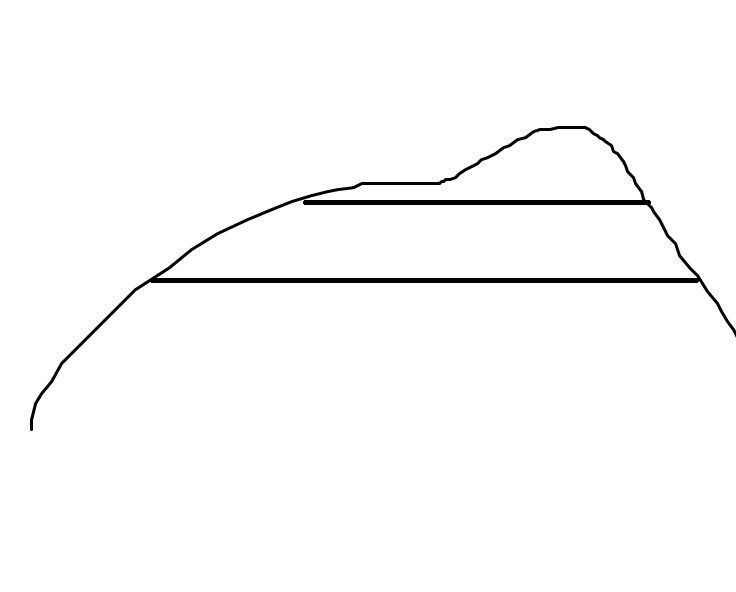
\includegraphics[width=0.5\textwidth]{graphic_example}
%\end{figure*}

\subsection{Introduction}

We want to generalize the notion of the \textit{length} towards all 
the subsets of $\mathbb{R}$.
Such a generalized function is usually called \textit{measure}.
But, unfortunately, such a function does not exist.

\begin{theorem}
\label{the:measureNotExists}
    There exist no such function $\mu: 2^{[0,1]} \to [0, +\infty)$ that satisfies the 
    following properties:
    \begin{enumerate}
        \item {
            The function is non-negative;
        }
        \item {
            It's countably additive;
        }
        \item {
            It's monotonic: the measure of a subset is not greater than the entire set;
        }
        \item {
            Translation does not change the measure;
        }
        \item {
            The measure of the unit interval is 1.
        }
    \end{enumerate}
\end{theorem}

\begin{proof}
    First, several definitions:
    \begin{enumerate}[label={Step \arabic*.}]
        \item {
            Let's define the following equivalence relation:
            if $x$, $y$ are from the unit interval, we'll say that
            $x \sim y$ if $x - y \in \mathbb{Q}$.
        }
        \item {
            Let's choose $N \subset [0, 1/3]$ such that it contains
            \textit{precisely one} element from each equivalence class.
            (Such an $N$ exists if the axiom of choice holds true).
        }
        \item {
            For all $r \in \mathbb{Q}$ define $N_r = N + r$.
        }
    \end{enumerate}

    \begin{itemize}%[font={\bfseries}]
        \item[Claim 1.] {
            The sets $N_R$ are congruent to $N$ and are pairwise disjoint.
        }
        \item[Proof.] {
            The sets are congruent by definition. Let's prove that 
            they are pairwise disjoint.

            Assume that $x \in N_{r_1} \cap N_{r_2}$ for some
            $r_1, r_2 \in \mathbb{Q}$.
            Then $x - r_1 \in N$, $x - r_2 \in N$, but
            $(x - r_1) \sim (x - r_2) \implies r_1 = r_2$.
        }
        \item[Claim 2.] {
            \[
                \Bigl[\frac{1}{3}, \frac{2}{3}\Bigr] \in
                \bigcup_{r \in \mathbb{Q} \cap [0, 2/3]} N_r
            \]
        }
        \item[Proof.] {
            If $x \in [1/3, 2/3]$, then
            $\exists!\, y \in N$ such that $x = y + q$ for some $q \in \mathbb{Q}$,
            as $N$ contains exactly one representative from each of the equivalence classes.
            It is easy to see that such $q \in [0, 2/3]$.
        }
    \end{itemize}

    We arrive at the following conclusion:
    \[
        \frac{1}{3} = \mu\bigl([1/3, 2/3]\bigr) \le \mu\Bigl( \bigcup_{r \in \mathbb{Q} \cap [0, 2/3]} N_r \Bigr) = 
        \sum_{r \in \mathbb{Q} \cap [0, 2/3]} \mu(N_r) \le 1
    \]
    What is $\mu(N)$ then? If $\mu(N) = 0$, then 
    \[
        \mu\Bigl( \bigcup_{r \in \mathbb{Q} \cap [0, 2/3]} N_r \Bigr) = 
        \sum 0 = 0
    \]
    If $\mu(N) = \varepsilon > 0$, then the sum is $+\infty$. 
    But it's supposed to be in $[1/3, 1]$?!
\end{proof}

\begin{consequence}
    We cannot generalize the notion of length to all subsets of real numbers.
\end{consequence}

\subsection{Lebesgue Outer Measure}
\begin{definition}
    If $I \subset \mathbb{R}$ is an interval, then
    $l(I) = \text{the length of $I$}$. If $I$ is unbounded, then $l(I) = \infty$.
\end{definition}
\begin{definition}[Outer Measure]
    \begin{align*}
        &
        m^* : 2^{\mathbb{R}} \to [0, +\infty]
        \\&
        m^*(A) = \inf \Bigl\{ \sum_{j = 1}^{\infty} l(I_j) \mid 
        I_j \text{ --- open intervals},\ A \subseteq \bigcup_{j=1}^{\infty} I_j\Bigr\}
    \end{align*}
    In words, it's the infimum of all \textit{countable} covers of $A$.
    (A countable sum either converges or diverges to infinity).
\end{definition}
\begin{remark}
    This is certainly not a measure --- otherwise, it would contradict Theorem~\ref{the:measureNotExists}.
\end{remark}

\begin{example}
    If $A$ is countable, then $m^*(A) = 0$.
\end{example}
\begin{proof}
    Let's choose an arbitrary $\varepsilon > 0$ and prove that $m^*(A) \le 2\varepsilon$.
    Let's choose a cover of the points with segments of lengths $\varepsilon$, $\varepsilon / 2$, $\varepsilon / 2^2$, and so on.
    Then \[
        m^*(A) = \inf \{\dots\} \le \varepsilon + \frac{\varepsilon}{2} + \frac{\varepsilon}{2^2} + \dots = 2\varepsilon
    \]
\end{proof}

\begin{proposition}
    If $A$ is an interval, then $m^*(A) = l(A)$.
\end{proposition}
\begin{proof}
    \begin{enumerate}[label=\alph*)]
        \item {
            $A$ is a closed interval, $A = [a, b]$.
            \begin{enumerate}[label=\arabic*.]
                \item {
                    $m^*(A) \le b - a$.
                    To prove this, we can cover $A$ with a single interval:
                    \[ (a - \varepsilon, b + \varepsilon) \implies \sum l(I_j) = b - a + 2\varepsilon \]
                    Now take $\varepsilon \to 0$.
                }
                \item {
                    $m^*(A) \ge b - a$.
                    Suppose we an infinite cover of $A$ by open intervals.
                    Since $A$ is a compact set, we can choose a finite subcover.
                    The case of a finite cover with open intervals is simple.
                    We can prove it as follows: if we have two intersecting 
                    open intervals, we can replace them with a single interval
                    of a lesser length. Then we can continue this process using induction.
                }
            \end{enumerate}
        }
        \item {
            If $A$ is unbounded, then all of the covers would have infinite sum, and thus 
            the infimum will be infinite as well.
        }
        \item {
            If $A$ is an open or semiclosed interval, we can approximate it from both sides
            by closed intervals.

            Let's denote the closure of $A$ by $\bar{A}$.
            Since we're adding points, the Outer Measure will not decrease:
            \[ A \subset \overline{A} \implies m^*(A) \le m^*(\overline{A}) = l(a) \]

            \pagebreak
            Now suppose we have a closed interval $B$ strictly inside $A$. Then we get
            \[ m^*(A) \ge m^*(B) = l(B) = l(A) - \varepsilon \]
            Now take $\eps \to 0 \implies m^*(A) \ge l(A)$.

            \begin{figure*}[h]
                \centering
                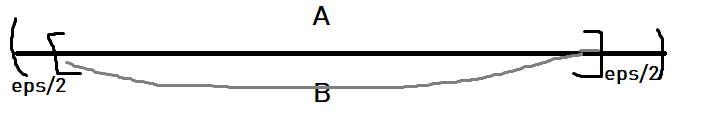
\includegraphics[width=0.5\textwidth]{measure_a_and_b}
            \end{figure*}
        }
    \end{enumerate}
\end{proof}
\begin{lemma}
    $m^*$ is translation-invariant.
\end{lemma}
\begin{proof}
    If we translate the set, we can translate all of its 
    covers as well. Since translating an interval does not
    change its length, the lengths of the covers won't change either.
\end{proof}

\begin{proposition}[Countable subadditivity]
    \label{the:countableSubadditivity}
    For any countable collection of sets
    $\{E_k\}_{k=1}^\infty$ we have 
    \[ m^*\Bigl(\bigcup_{k=1}^\infty E_k\Bigr) \le \sum_{k=1}^\infty m^*(E_k) \]
\end{proposition}
\begin{remark}
    We don't ask for the sets $E_k$ to be disjoint. 
    If we proved that we have an equality sign for the disjoint case,
    we would have proved that $m^*$ is a measure, which we proved does not exist
    in Theorem~\ref{the:measureNotExists}.
\end{remark}
\begin{proof}
    Choose open intervals $I_{k,i}$, such that
    \[E_k \in \bigcup_{i=1}^\infty E_{k,i} \text{ ($E_{k, i}$ are a cover of $E_k$)}\] and
    \[\sum_{i=1}^\infty l(I_{k,i}) < m^*(E_k) + \frac{\varepsilon}{2^k}\]
    Such intervals exist from the definition of the infimum.

    On the other hand, $\{ I_{k,i} \mid 1 \le k, i < \infty \}$
    covers each of the $E_k$, and thus it's a cover of
    $\cup_{k=1}^\infty E_k$.
    Then 
    \[ 
        m^*\Bigl(\bigcup_{k=1}^\infty E_k\Bigr) \overset{\text{it's a cover}}{\le}
        \sum_{1 \le k, i < \infty} l(I_{k,i}) <
        \sum_{k=1}^\infty m^*(E_k) + \varepsilon \Bigl(\frac{1}{2} + \frac{1}{4} + \dots\Bigr) =
        \sum_{k=1}^\infty m^*(E_k) + \varepsilon
    \]
    Now take $\varepsilon \to 0$.
\end{proof}
\begin{remark}
    Here we assume that all of the $E_k$ have finite outer measures.
    Otherwise, both of the sides of the inequality would diverge
    to infinity, and we get $\infty \le \infty$ which is ``true''.
\end{remark}

\pagebreak
\subsection{The $\sigma$-algebra of Lebesgue-measurable sets.}
\begin{definition}
    A set $E$ is (Lebesgue) measurable if for any set 
    $A$,
    \[ 
        m^*(A) = m^*(A \cap E) + m^*(A \cap E^{C})
        \qquad E^C = \mathbb{R} \setminus E
    \]
    \begin{figure*}[h]
        \centering
        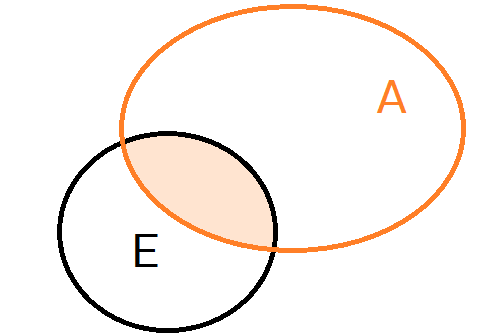
\includegraphics[width=0.3\textwidth]{measure_e_and_a}
        \caption{The set $E$ ``splits'' $A$ into two parts}
    \end{figure*}
\end{definition}
\begin{remark}
    We already have the $\le$ sign from Proposition~\ref{the:countableSubadditivity}.
\end{remark}
\begin{remark}
    Motivation: If $A \cap B = \emptyset$ and $A$ (or $B$) is measurable, then
    \[
        m^*(A \cup B) = m^*\bigl((A \cup B) \cap A\bigr) +
        m^*\bigl( (A \cup B)  \cap A^C \bigr) = m^*(A) + m^*(B)
    \]
\end{remark}

\begin{proposition}
    If $m^*(E) = 0$, then $E$ is measurable.
\end{proposition}
\begin{proof}
    For all $A$ we have:
    \begin{align*}
        &
        m^*(A \cap E) \le m^*(E) = 0 \implies m^*(A \cap E) = 0
        \\&
        m^*(A) \ge m^*(A \cap E^C) = m^*(A \cap E) + m^*(A \cap E^C)
    \end{align*}
    As we noted earlier, the inequality in the other side follows from 
    Proposition~\ref{the:countableSubadditivity}.
\end{proof}

% TODO make it Proposition 2 as in the second proposition in subsection.
\begin{proposition}  
    If $E_1, \dots, E_n$ are measurable, then 
    $\cup_{1}^n E_k$ is measurable.
\end{proposition}
\begin{proof}
    Case $n=2$:
    for all $A$ we have
    \begin{align*}
        &
        m^*(A) = m^*(A \cap E_1) +  m^*(A \cap E_1^C)
        =\\&=
        m^*(A \cap E_1) + m^*\bigl((A \cap E_1^C) \cap E_2\bigr) +
        m^*\bigl((A \cap E_1^C) \cap E_2^C\bigr) = (*)
        \\&
        X := A \cap E_1,\
        Y := (A \cap E_1^C) \cap E_2,\
        Z := (A \cap E_1^C) \cap E_2^C
    \end{align*}
    With Venn diagrams it's possible to prove that 
    $Z = A \cap (E_1 \cup E_2)^C$, $X \cup Y = A \cap (E_1 \cup E_2)$.
    Now let's apply Proposition~\ref{the:countableSubadditivity} to $X$ and $Y$. Then we get:
    \[
        (*) \ge m^*\bigl(A \cap (E_1 \cup E_2)\bigr) +
        m^*\bigl(A \cap (E_1 \cup E_2)^C\bigr)
    \]

    Induction step:
    Apply case $n=2$ to the sets 
    $\cup_{1}^{n - 1} E_k$, $E_n$.
\end{proof}
\textbf{Summary of Taylor series:}
\begin{itemize}
    \item {
        Problem: Evaluate $f(x)$ with a given error bound.
    }
    \item {
        Required: $f \in \mathrm{C}^{n+1}$, values of derivatives $f^{(k)}(a)$.
    }
    \item {
        Check interval of convergence: does Taylor series expansion work?
    }
    \item {
        Estimate the maximum error for $n$ terms of the Taylor polynomial.
    }
    \item {
        Choose $n$, such that the error bound is low enough.
    }
    \item {
        Evaluate the Taylor polynomial.
    }
\end{itemize}

\newpage
\section{Number representation}

\subsection{Errors}
There are different error types:
\begin{enumerate}
    \item {
        An error in data (partly due to roundoff).
    }
    \item {
        Roundoff errors (during computation). For example,
        multiplication increases the amount of needed significant digits, and
        we can't store them all on a computer.
    }
    \item {
        Truncation error, that is inherent to numeric methods. For example,
        if we take a finite number of terms in our Taylor series.
    }
\end{enumerate}

\begin{definition}
    Let $\tilde{a}$ be an approximation of $a$. Then
    $\abs{\tilde{a} - a}$ is the \textit{absolute error}, and 
    $\abs{\frac{\tilde{a} - a}{a}}$ is the \textit{relative error}.
    The \textit{error bound} is the magnitude of admissable error.
\end{definition}
\begin{example}
    0.00123 with error $0.000004 = 0.4 \cdot 10^{-5}$.
    The error is below $\frac{1}{2} \cdot 10^{-t}$ with $t = 5$, so there's 5
    correct digits and 3 significant digits (the number of non-leading zeros).
\end{example}
\begin{example}
    0.00123 with error $0.000006 = 0.06 \cdot 10^{-4} > \frac{1}{2} \cdot 10^{-5}$.
    Only has 2 significant digits, because we have to round the error up.
\end{example}

\begin{theorem}
    In addition/subtraction the bounds for absolute errors are added,
    in multiplication/division the relative errors are added.
\end{theorem}
\begin{example}
    Solve $x^2 - 56x + 1 = 0$:
    \[
        x = 28 - \sqrt{783} \approx 28 - 27.982 \text{ (5 significant digits)} =
        0.018 \pm \frac{1}{2} \cdot 10^{-3}
    \]
    We end up with 2 significant digits in the answer, despite that we used to 
    have 5. That's why computers use floating point numbers, as
    leading zeros are bad.
\end{example}

\begin{definition}[Error propagation]
    If $y(x)$ is smooth, than the derivative $\abs{y(x)'}$
    can be interpreted as the sensitivity of $y(x)$ to errors in $x$.
    We can generalize this to functions of multiple variables:
    \[
        \abs{\Delta y} \le \sum \abs{\frac{\partial y}{\partial x_i}} \cdot \abs{\Delta x_i}
        \text{, where } \Delta y = \tilde{y} - y,\ \Delta x_i = \tilde{x_i} - x_i
    \]
    This is an empirical inequality that is only valid for small $\Delta x_i$.
    It is used a lot in physics.
\end{definition}

\subsection{Base representation}
\begin{definition}[Base representation]
    Every number $x \in \mathbb{N}$ can be written in the following form 
    as a unique expansion with respect to the base $b$, where
    $b \in \mathbb{N} \setminus \{1\}$:
    \begin{align*}
        &
        x = a_0 b^0 + a_1 b^1 + a_2 b^2 + \dots + a_n b_n = 
        \sum_{i=0}^n a_i b^i 
        \\&
        a \in \mathbb{N}_0,\ a_i < b,\ a_i \in \{0, \dots, b - 1\}
    \end{align*}
        
    Here $b$ is called the \textit{base}, $a_i$ are called the \textit{digits}.
    Humans usually use base 10. But, for example, computers
    can use base 2.

    For a real number $x \in \mathbb{R}$ we can write: 
    \[
        x = \sum_{i=0}^n a_i b^i + \sum_{i=1}^\infty a_{-i} b^{-i}
    \]
\end{definition}
\begin{example}
    $b=2:\ 1011 = 1 \cdot 2^0 + 1 \cdot 2^1 + 0 \cdot 2^2 + 1 \cdot 2^3 =
    (11)_{10}$
\end{example}
There are different algorithms that convert number systems.

\subsection{Euclid's algorithm}
Euclid's algorithm converts $(x)_{10}$ to $(y)_b$.
\begin{enumerate}%[label={\arabic*)}]
    \item {
        Input $(x)_{10}$.
    }
    \item {
        Determine the smallest $n$, such that $x < b^{n+1}$.
    }
    \item {
        For $i=n$ to $0$ do:
        \begin{align*}
            &
            a_i \coloneqq x\ \mathrm{div}\ b^{i} \text{ (integer division)}
            \\&
            x \coloneqq x\ \mathrm{mod}\ b^{i} \text{ (the remainder)}
        \end{align*}
    }
    \item {
        Output result $a_n a_{n-1} a_{n-2} \dots a_0 = (y)_b$.
    }
\end{enumerate}

\begin{example}
    \begin{enumerate}
        \item {
            $(x)_{10} = (13)_{10} \to (y)_2$
        }
        \item {
            $n = 3$ since $13 < 2^4$.
        }
        \item {
            \begin{align*}
                &
                i = 3:\ a_3 = 13 \ \mathrm{div}\ 2^3 = 1,\
                x = 13 \ \mathrm{mod}\ 2^3 = 5
                \\&
                i = 2:\ a_2 = 5 \ \mathrm{div}\ 2^2 = 1,\
                x = 5 \ \mathrm{mod}\ 2^2 = 1
                \\&
                i = 1:\ a_1 = 1 \ \mathrm{div}\ 2^1 = 0,\
                x = 1 \ \mathrm{mod}\ 2^1 = 1
                \\&
                i = 0:\ a_0 = 1 \ \mathrm{div}\ 2^0 = 1,\
                x = 1 \ \mathrm{mod}\ 2^0 = 0
            \end{align*}
        }
        \item {
             Output: $(1101)_2 = (13)_{10}$.
        }
    \end{enumerate}
\end{example}
Two problems of the Euclid's algorithm:
\begin{enumerate}
    \item {
        Step 2 is inefficient
    }
    \item {
        Division by large numbers can be problematic.
    }
\end{enumerate}

\subsection{Horner's scheme}
Horner's scheme is a more efficient algorithm. The idea is to represent
the number as follows:
\[
    (a_n a_{n - 1} \dots a_{0})_b = 
    a_0 + b\bigl(a_1 + b(a_2 + b(a_3 + \dots + b (a_n))) \dots \bigr)
\]
The algorithm is the following:
\begin{enumerate}
    \item {
        Input $(x)_{10}$.
    }
    \item {
        $i \coloneqq 0$.
    }
    \item {
        While $x > 0$ do:
        \begin{align*}
            &
            a_i \coloneqq x \ \mathrm{mod}\ b
            \\&
            x \coloneqq x \ \mathrm{div}\ b
            \\&
            i \coloneqq i + 1
        \end{align*}
    }
    \item {
        Output result $a_n a_{n-1} a_{n-2} \dots a_0 = (y)_b$.
    }
\end{enumerate}
\begin{remark}
    The algorithm is very similar to the Euclid's algorithm ---
    the difference is that we execute it in reverse. 
    We no longer have divisions by large numbers, and thus
    it runs faster.
\end{remark}

\textbf{General remarks:}
\begin{itemize}
    \item {
        A number with simple representation in one base 
        may be complicated to represent in another base.
        For example,
        $(0.1)_{10} = (0.0001100110011\dots)_2$.
    }
    \item {
        Base 2 is called \textit{binary},
        base 8 is \textit{octal},
        base 16 is \textit{hexadecimal}.
    }
    \item {
        To convert from a base $b$
        to base $10$ we can just perform the following computation:
        \[
            (42)_8 = 4 \cdot 8^1 + 2 \cdot 8^0 = (34)_{10}
        \]
    }
    \item {
        Conversion $2$ and $8$. $8=2^3$:
        three consecutive bits represent one octal digit, e.g.
        \[ (551.624)_8 = (101 101 001.110 010 100)_2 \]
    }
    \item {
        Conversion $2$ and $16=2^4$: just four bits to one hexadecimal digit. 
    }
    \item {
        Horner's scheme algorithm does not need estimate of $n$
        and does not divide by large numbers.
    }
    \item {
        It is applicable to real numbers, but one needs a critireon to stop
        if the representation with the new base is infinite.
    }
    \item {
        On computers we only have finite precision
        (the number of digits/bits).
    }
\end{itemize}
\begin{definition}[Measurable space]
    A \textit{measurable space} is a tuple $(X, \mathcal{A})$, where:
    \begin{enumerate}
        \item {
            $X$ is a set.
        }
        \item {
            $\mathcal{A}$ is a $\sigma$-algebra on $X$.
        }
    \end{enumerate}
\end{definition}

\begin{definition}[Measure space]
    A \textit{measure space} is a triple $(X, \mathcal{A}, \mu)$, where:
    \begin{enumerate}
        \item {
            $X$ is a set.
        }
        \item {
            $\mathcal{A}$ is a $\sigma$-algebra on $X$.
        }
        \item {
            $\mu$ is a measure on $(X, \mathcal{A})$.
        }
    \end{enumerate}
\end{definition}

\begin{example}[1]
    $\{\emptyset, X\}$ is a $\sigma$-algebra. Any $\mu$, such that
    $\mu(\emptyset) = 0$ and $\mu(X) \ge 0$ will be a measure.
\end{example}
\begin{example}[2]
    $2^X$ is a $\sigma$-algebra. We can have the following measures:
    \begin{enumerate}[label=\alph*)]
        \item {
            $\mu(E) = \abs{E}$ is called a \textit{counting measure}.
            Here $\abs{E}$ denotes the cardinality of $E$ (number of elements in $E$).
        }
        \item {
            $\delta$-measure (also called Dirac measure):
            \[
                \mu(E) = \begin{cases}
                    1, &0 \in E\\
                    0, &\text{otherwise}
                \end{cases}
            \]
        }
    \end{enumerate}
\end{example}

\subsection{Continuity of measure}

\begin{definition}
    A countable collection of sets $\{E_k\}_{k=1}^\infty$ is called
    \textit{ascending} if $E_k \subset E_{k+1}$.
\end{definition}
\begin{definition}
    A countable collection of sets $\{E_k\}_{k=1}^\infty$ is called
    \textit{descending} if $E_k \supset E_{k+1}$.
\end{definition}

\begin{theorem}[Continuity of measure]
    \label{the:continuityOfMeasure}
    \item{} % Newline hack
    \begin{enumerate}
        \item {
            If $\{A_k\}_{k=1}^\infty \subset \mathcal{A}$ and the sequence is ascending,
            then
            \[
                \mu\Bigl(\bigcup_{k=1}^\infty A_k\Bigr) = \lim_{k \to \infty} \mu(A_k)
            \]
        }
        \item {
            If $\{B_k\}_{k=1}^\infty \subset \mathcal{A}$, the sequence is descending and $\mu(B_1) < \infty$,
            then
            \[
                \mu\Bigl(\bigcap_{k=1}^\infty B_k\Bigr) = \lim_{k \to \infty} \mu(B_k)
            \]
        }
    \end{enumerate}
\end{theorem}
\begin{proof}
    \begin{enumerate}
        \item {
            Let $C_k \coloneqq A_k \setminus A_{k-1}$. Then we have:

            \begin{figure*}[h]
                \centering
                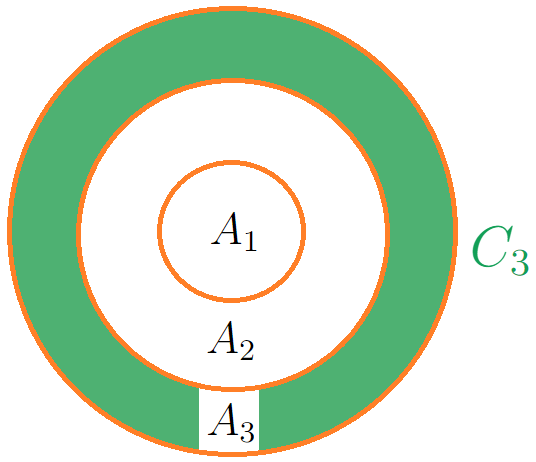
\includegraphics[width=0.3\textwidth]{a1a2a3}
            \end{figure*}

            \[
                \mu\Bigl(\bigcup_{k=1}^\infty A_k\Bigr) =
                \mu\Bigl(\bigsqcup_{k=1}^\infty C_k\Bigr) =
                \sum_{k=1}^\infty \mu(C_k) =
                \lim_{n \to \infty} \sum_{k=1}^n \mu(C_k) = \lim_{n \to \infty} \mu(A_n)
            \]
        }
        \item {
            Let $D_k \coloneqq B_1 \setminus B_k$. 
            Since $B_k$ is descending, it follows that $D_k$ is an ascending sequence. Then from the part 1 of the theorem it follows that:
            \begin{align*}
                &
                \mu\Bigl(\bigcup_{k=1}^\infty D_k\Bigr) = \lim_{k \to \infty} \mu(D_k)
                \qquad
                \bigcup_{k=1}^\infty D_k = B_1 \setminus \bigcap_{k=1}^\infty B_k
                \\&
                \mu\Bigl(B_1 \setminus \bigcap_{k=1}^\infty B_k\Bigr) =
                \lim_{k \to \infty}\bigl(\mu(B_1) - \mu(B_k)\bigr) =
                \mu(B_1) - \lim_{k \to \infty} \mu(B_k)
                \\&
                \mu\Bigl(B_1 \setminus \bigcap_{k=1}^\infty B_k\Bigr) =
                \mu(B_1) - \mu\Bigl(\bigcap_{k=1}^\infty B_k\Bigr) \implies
                \mu\Bigl(\bigcap_{k=1}^\infty B_k\Bigr) = \lim_{k \to \infty} \mu(B_k)
            \end{align*}
        }
    \end{enumerate}    
\end{proof}

\begin{definition}
    We say that a statement (property) holds for \textit{almost all} $x \in X$
    \textit{with respect to a measure $\mu$}, if
    $\exists N \in \mathcal{A}$, such that $\mu(N) = 0$ and the statement (property)
    holds for all $x \in X \setminus N$.
\end{definition}
\begin{lemma}[Borel–Cantelli]
    Let $(X, \mathcal{A}, \mu)$ be a measure space. Let
    $\{E_k\}_{k=1}^\infty \subset \mathcal{A}$ and $\sum_{k=1}^\infty \mu(E_k) < \infty$.
    Then \textit{almost all} $x \in X$ belong to at most finitely many $E_k$.
\end{lemma}
\begin{proof}
    Let $B_n = \cup_{k=n}^\infty E_k$. It's easy to see that $B_k$ is a descending measure.
    At the same time,
    \[ \mu(B_1) = \mu\Bigl(\bigcup_{k=1}^\infty E_k\Bigr) \le \sum_{k=1}^\infty \mu(E_k) < \infty \]
    By definition of $B_n$, $\cap_{n=1}^\infty B_n$ contains all the points
    that are contained in infinitely many $E_k$'s. But, by \hyperref[the:continuityOfMeasure]{continuity of measure} 
    for $\{B_n\}_{n=1}^\infty$ we have:
    \[ 
        \mu\Bigl(\bigcap_{n=1}^\infty B_n\Bigr) =
        \lim_{n \to \infty} \mu(B_n) =
        \lim_{n \to \infty} \Bigl(\bigcup_{k=n}^\infty E_k\Bigr) \le
        \lim_{n \to \infty} \sum_{k=n}^\infty \mu(E_k) = 0
    \]
\end{proof}

\subsection{How large is the Lebesgue $\sigma$-algebra $\mathcal{M}$?}
\begin{proposition}
    \label{prop:intervalsAreMeasurable}
    Every interval is Lebesgue-measurable.
\end{proposition}
\begin{proof}
    Proof idea:
    \[ 
        E \in \mathcal{M} \Longleftrightarrow 
        \forall A: m(A) = m(A \cap E) + m(A \cap E^C)
    \]
    Assume $E = (-\infty, a)$. If we prove that such intervals lie in $\mathcal{M}$, 
    then we'll prove everything (since $\mathcal{M}$ is a $\sigma$-algebra).
    We already have $m(A) \le m(A \cap E) + m(A \cap E^C)$ from \hyperref[the:countableSubadditivity]{countable subadditivity}.

    Let's assume $a \not\in A$ (since removing one point does not change the measure).
    Every cover of $A$ can be split into two covers with the same sum of interval lengths: of
    $A \cap (-\infty, a)$ and $A \cap (a, +\infty)$. Every interval in those
    covers, that contains $a$, can be split into two. Therefore,
    from the \hyperref[def:lebesgueOuterMeasure]{definition of Lebesgue measure}, 
    $m(A) \ge m(A \cap E) + m(A \cap E^C)$, so we've proved the inequality in both sides.
\end{proof}
\begin{definition}
    For any $\mathcal{X} \in 2^\mathbb{R}$ let $\mathcal{A}(\mathcal{X})$
    be the smallest $\sigma$-algebra containing $\mathcal{X}$.
\end{definition}

\begin{lemma}
    $\mathcal{A}(\mathcal{X})$ always exists and is the intersection of all $\sigma$-algebras
    containing $\mathcal{X}$.
\end{lemma}
\begin{proof}
    We have to prove that if we intersect a bunch $\sigma$-algebras, we still get a 
    $\sigma$-algebra.
    \begin{enumerate}
        \item {
            Such an intersection is closed under complements:
            if a set belongs to the intersection of $\sigma$-algebras,
            then it belongs to each of the $\sigma$-algebras, 
            then its complement belongs to each of the $\sigma$-algebras,
            and thus its complement belongs to the intersection of 
            $\sigma$-algebras.
        }
        \item {
            In a similar way, such an intersection is closed under countable unions:
            if a number of sets all belong to the intersection of $\sigma$-algebras,
            then they all belong to each of the $\sigma$-algebras, 
            then their countable union belongs to each of the $\sigma$-algebras,
            and their countable union belongs to the intersection of 
            $\sigma$-algebras.
        }
    \end{enumerate}
\end{proof}

\begin{remark}
    We can try to construct $\mathcal{A}(\mathcal{X})$ in a different way.
    Say, $\mathcal{X}$ is not a $\sigma$-algebra. Let's enlarge it:
    first by including all the complements. Then let's enlarge it
    by all countable unions. Let's call such a set $\mathcal{X}_1$.
    But after such operation, $\mathcal{X}_1$ may be non-closed under complements.
    So we repeat such a procedure.

    And, in general: $\mathcal{X}_{n + 1}$ is obtained from $\mathcal{X}_n$
    is obtained by including into $\mathcal{X}_n$ all complements of the 
    sets from $\mathcal{X}_n$ and then including all countable unions of the obtained sets.

    \begin{figure*}[h]
        \centering
        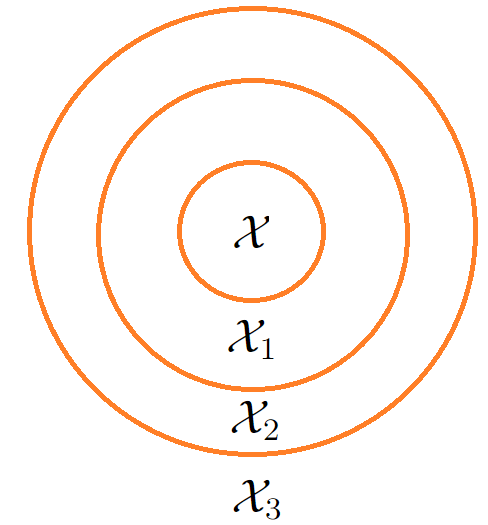
\includegraphics[width=0.3\textwidth]{some_circles}
    \end{figure*}

    It is tempting to think that $\cup_{1}^\infty \mathcal{X}_i$ is $\mathcal{A}(\mathcal{X})$.
    Is it true? No, not necessarily.
    If the sequence $\{\mathcal{X}_i\}$ eventually stabilizes, then such a construction works.
    Let's now assume that every next $\mathcal{X}_i$ is larger than the previous one.
    Then we can take $A$ from $\mathcal{X}$, $A_1$ from $\mathcal{X}_1 \setminus \mathcal{X}$,
    $A_2$ from $\mathcal{X}_2 \setminus \mathcal{X}_1$, and so on.

    Now let's look at $\cup_{1}^\infty A_i$. As a countable union, it must be contained
    in $\mathcal{A}(\mathcal{X}) = \cup_{1}^\infty \mathcal{X}_i$, thus, there exist an $n$, such that
    $\cup_{1}^\infty A_i \in \mathcal{X}_n$. But $A_{n+1} \in \mathcal{X}_{n+1} \setminus \mathcal{X}_n$?!
\end{remark}

\begin{definition}[Topological space]
    A \textit{topological space} is a set $X$ and a collection
    of subsets $O$ of $X$ (called \textit{open sets}), such that $\emptyset, X \in O$, and:
    \begin{enumerate}
        \item {
            A union of (possibly infinitely many) sets from $O$
            is in $O$.
        }
        \item {
            The intersection of finitely many sets from $O$
            is in $O$.
        }
    \end{enumerate}
    The complements of open sets are called \textit{closed sets}.
\end{definition}

\begin{definition}
    A function $f : X \to Y$ between two topological spaces is \textit{continuous} if
    the preimage of every open set is open.
\end{definition}
\begin{remark}
    It is possible to check that for $\mathbb{R}$ this definition is
    equivalent to the usual one.
\end{remark}

\begin{definition}[Borel $\sigma$-algebra]
    For a topological space $X$ its \textit{Borel $\sigma$-algebra $\mathcal{B}_X$}
    is the smallest $\sigma$-algebra on $X$ that contains all open sets. 
\end{definition}
\begin{remark}
    If it's obvious from the context which set we are talking about,
    we will just write $\mathcal{B}$ (without a subscript).
\end{remark}

\begin{theorem}
    \label{the:openMeasurable}
    $\mathcal{B}_\mathbb{R} \subset \mathcal{M}$ (all of the sets in $\mathcal{B}_\mathbb{R}$ are measurable).
\end{theorem}
\begin{proposition}
    \label{prop:bIsSmallestSigmaAlgebra}
    $\mathcal{B}$ is the smallest $\sigma$-algebra that contains all open intervals.
\end{proposition}
If we prove the proposition, the theorem will follow easily.
We know that \hyperref[prop:intervalsAreMeasurable]{all the intervals are Lebesgue-measurable}.
We know that the Lebesgue-measurable sets ($\mathcal{M}$) 
\hyperref[the:mIsSigmaAlgebra]{are a $\sigma$-algebra}.
Thus, if we take the smallest $\sigma$-algebra that contains all open intervals,
it will be a subset of $\mathcal{M}$.
\begin{proof}[Proof of Proposition~\ref{prop:bIsSmallestSigmaAlgebra}]
    We will prove that every open set $O \subset \mathbb{R}$ is a finite or
    countable union of open intervals.

    For every point $x \in O$ let $I_x$ be the largest open interval, such that
    $x \in I_x$ and $I_x \subset O$.
    It exists as a union of all such intervals. Since $O$ is open, 
    $x$ lies in $O$ with an open neighborhood,
    thus, $I_x$ is non-empty.
    \[
        \forall x \in O: x \in I_x \implies
        O = \bigcup_{x \in O} I_x
    \]
    Let's prove that $I_x \cap I_y \ne \emptyset \implies I_x = I_y$. If the intervals
    around $x$ and $y$ intersect, then $I_x \cup I_y$ is an interval as well, and
    $I_x \cup I_y \in O$ as $I_x \in O$ and $I_y \in O$. Since $I_x$ and $I_y$ are the largest such intervals, it follows that
    $I_x = I_x \cup I_y = I_y$.

    Let's say that two points $x$ and $y$ are equivalent if $I_x = I_y$.
    Since there's a lot of same intervals in $O = \cup_{x \in O} I_x$,
    we can take just a single point from every equivalence class and still get $O$ 
    as a union. Particularly, every open interval contains at least one rational point
    (as rational numbers are dense). Therefore, there's a rational point
    in every equivalence class.
    Thus,
    \[ O = \bigcup_{x \in O \cap \mathbb{Q}} I_x \]
    Since the set of rational numbers is countable, we have represented $O$
    as a countable union of open intervals, which is what we wanted.
\end{proof}

\begin{remark}
    A topological space is called \textit{separable}, if it contains a 
    countable dense subset.
\end{remark}
\begin{remark}
    We have proved that the Lebesgue measure exists on $\mathcal{B}_\mathbb{R}$,
    so we have a lot of measurable sets.
\end{remark}
\begin{remark}
    The Lebesgue measure can be generalized to $\mathbb{R}^n$.
\end{remark}
\pagebreak
\subsection{Other critirea of measurability for Lebesgue measure}
As we remember, \hyperref[def:measurable]{the definition
of a measurable set} is difficult to check. Thus, we would like to have
better critirea.
\begin{theorem}
    $E \subset \mathbb{R}$ is Lebesgue measurable if and only if one of the following holds:
    \begin{enumerate}
        \item {
            For every $\varepsilon > 0$ there exists an open set $O$, such that
            $E \subset O$ and $m^*(O \setminus E) < \varepsilon$.
        }
        \item {
            There exists a $G_\delta$-set $G$, such that $E \subset G$ 
            and $m^*(G \setminus E) = 0$.

            (A $G_\delta$-set is a countable intersection of open sets.)
        }
        \item {
            For every $\varepsilon > 0$ there exists a closed set $F$, such that
            $F \subset E$ and $m^*(E \setminus F) < \varepsilon$.
        }
        \item {
            There exists a $F_\sigma$-set $F$, such that $F \subset E$
            and $m^*(E \setminus F) = 0$.

            (A $F_\delta$-set is a countable union of closed sets.)
        }
    \end{enumerate}
\end{theorem}
\begin{proof}
    \mbox{}
    \begin{itemize}
        \item {
            $E$ is measurable $\implies$ 1.

            If $m^*(E) < \infty$, then from the definition of $m^*$
            we can find $O$ --- a finite union of open intervals, such that
            $m^*(O) < m^*(E) + \varepsilon$. Since $O$ is an open set, it's
            measurable (as we proved \hyperref[the:openMeasurable]{earlier}).
            Therefore, both $E$ and $O$ are measurable, thus
            \[ \varepsilon > m^*(O) - m^*(E) \overset{E, O \in \mathcal{M}}{=} m^*(O \setminus E) \]

            If $m^*(E) = \infty$, let's split the set $E$ into a countable number of sets with
            finite measure. For example, by splitting the real line into 
            segments of length 1. So,
            $E = \cup_1^\infty E_k$, where $m^*(E_k) < \infty$.
            Then let's use geometrically decreasing $\varepsilon$'s for the covers of each
            $E_k$: $\varepsilon / 2$ for $E_1$, $\varepsilon / 4$ for $E_2$, and so on.
            When we sum up the inequalities, the fractions will sum up to $\varepsilon$.
            So, we obtained our $O$, now continue like in the previous case.
            \begin{definition}
                A measure $\mu$ on $X$ is called 
                \textit{$\sigma$-finite}, if $X = \cup_1^\infty X_k$ and
                $\mu(X_k) < \infty$ for all $k$. 
                
                In words:
                if there exists a subdivision of $X$ into a countable number
                of set of finite measure.
            \end{definition}
        }
        \item {
            $1 \implies 2$.

            From $1$, $\forall k \in \mathbb{N},\ \exists O_k$ ---
            open, such that $E \subset O_k$ and
            $m^*(O_k \setminus E) < \frac{1}{k}$.
            Now let's take
            \[
                G \coloneqq \bigcap_1^\infty O_k \implies
                \forall k:\ m^*(G \setminus E) \le m^*(O_k \setminus E) < \frac{1}{k}
                \implies m^*(G \setminus E) = 0
            \]
        }
        \item {
            $2 \implies E$ is measurable.

            $G$ is a $G_\delta$-set. As a countable intersection of open sets,
            it's in Borel $\sigma$-algebra, and thus is Lebesgue-measurable.
            $m^*(G \setminus E) = 0$, then $G \setminus E$ is Lebesgue-measurable,
            then $E = G \setminus (G \setminus E)$ is measurable as
            a difference of two measurable sets.
        }
        \item {
            $3 \Longleftrightarrow 1,\ 4 \Longleftrightarrow 2$.

            If we assume that 3 holds for $E$, then, if we take $O = \overline{F}$,
            1 will hold for $\overline{E}$.
            Therefore, $\overline{E}$ is measurable, then $E$ is measurable
            (as $\mathcal{M}$ is a $\sigma$-algebra).

            If 1 holds for $E$, then $E$ is measurable, then $\overline{E}$ is measurable, then 1 holds for 
            $\overline{E}$. Now take $F = \overline{O}$, therefore, 3 holds for $E$.

            \begin{figure*}[h]
                \centering
                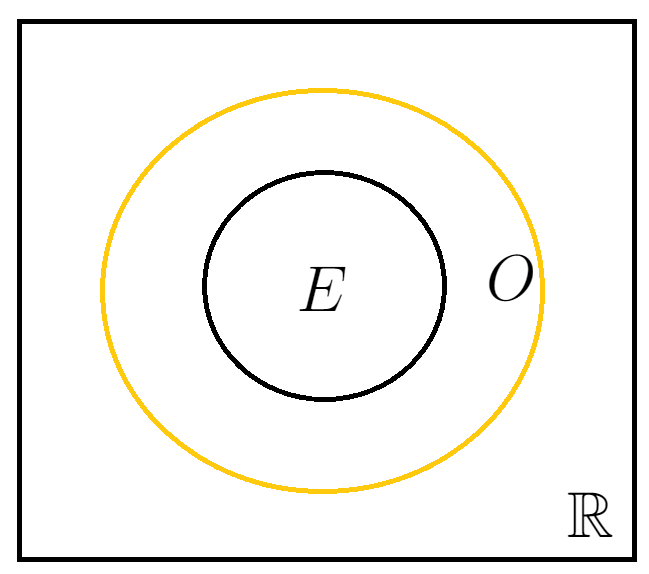
\includegraphics[width=0.3\textwidth]{e_o_r}
            \end{figure*}

            In the same way, 2 and 4 are equivalent as well.
        }
    \end{itemize}
\end{proof}

\begin{theorem}
    For every $E \in \mathcal{M}$ with $m(E) < \infty$ and for every
    $\varepsilon < \infty$ there exists an infinite disjoint collection of open intervals
    $\{I_k\}_1^n$, such that $O = \cup_{k=1}^n I_k$ and $m(E \triangle O) < \varepsilon$.

    (Here $\triangle$ is the symmetric difference of two sets).
\end{theorem}
\begin{proof}
    From part 1 of the previous theorem,
    we can take such an open set $U$, that $E \subset U$ and $m(U \setminus E) < \varepsilon / 2$. 
    
    As we proved \hyperref[prop:bIsSmallestSigmaAlgebra]{earlier}, 
    we can represent $U$ as a countable union of disjoint open intervals $I_k$. Then:
    \[
        \forall n: \bigcup_1^n I_k \subset U \implies \forall n:
        \sum_1^n m(I_k) \le m(U) < \infty
    \]
    Now take $n$, such that $\sum_{n+1}^\infty m(I_k) < \varepsilon / 2$, and put
    $O \coloneqq \cup_{k=1}^n I_k$.
    Then $m(O \setminus E) < \varepsilon / 2$ and $m(E \setminus O) < \varepsilon / 2$,
    therefore, the measure of the symmetric difference is less that $\varepsilon$.
\end{proof}

\subsection{Cantor set}

Questions:
\begin{enumerate}
    \item {
        If $m(A) = 0$, is $A$ countable?
    }
    \item {
        We know that $\mathcal{B} \subset \mathcal{M}$. Is this inclusion proper?
    }
\end{enumerate}

\begin{definition}[Cantor set]
    Let's take $[0, 1]$, split it into three parts and remove the middle part.
    Then continue such process.
    The \textit{Cantor set} is the set $C \coloneqq \cap_0^\infty C_k$.
\end{definition}

\begin{figure*}[h]
    \centering
    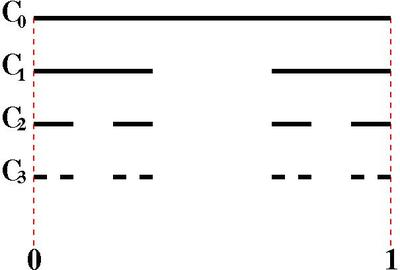
\includegraphics[width=0.3\textwidth]{cantor_set}
    \caption*{Cantor set illustration from \href{http://tasks.illustrativemathematics.org/content-standards/tasks/929}{here.}}
\end{figure*}

\begin{remark}
    The measure of $C_n$ is $(2/3)^n = 0$. From the
    \hyperref[the:continuityOfMeasure]{continuity of measure},
    the measure of the intersection is the limit of measures of individual sets,
    and thus $m(C) = 0$.
\end{remark}

\begin{remark}
    The Cantor set is countable,
    because if we have a sequence of zeros and ones, we can traverse 
    down-left on 0 and down-right on 1. The intersection of the corresponding
    intervals will be a single point of $C$. So, there's a bijection between
    $C$ and $\{0, 1\}^\mathbb{N}$, therefore, $C$ is indeed uncountable. 
\end{remark}

\begin{remark}
    Usually, when we remove the middle intervals on each step,
    we keep the end points.
    If we choose to remove the end points, we essentially remove
    the points that correspond to sequences that end with an infinite
    sequence of 0's or an infinite sequence of 1's. 
    It's clear that not all sequences of 0's and 1's are like that, 
    so there is going to be plenty of points left in the Cantor set, anyway.
\end{remark}

\begin{definition}[The Cantor function]
    The Cantor function $\varphi: [0, 1] \to [0, 1]$ is defined as follows.
    Let's first take the unit interval $[0, 1]$, split it in three,
    and define $\varphi$ to be $\frac{1}{2}$ on $[1/3, 2/3]$. Then let's continue the same
    with $[0, 1/3]$ and $[2/3, 1]$, and so on.

    \begin{figure*}[h]
        \centering
        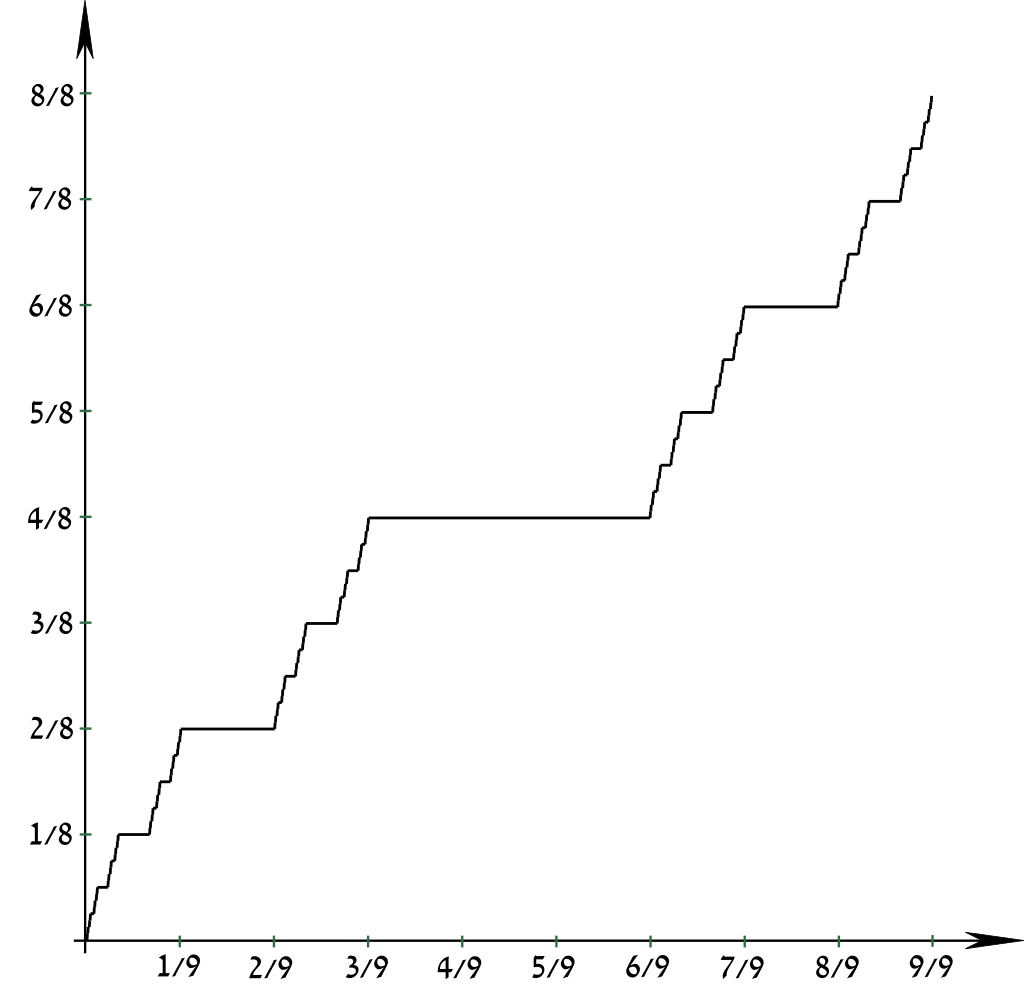
\includegraphics[width=0.4\textwidth]{cantor_function}
    \end{figure*}

    Now we have defined $\varphi$ for all points on the Cantor set. Here's
    how we'll define it on all others:
    \begin{align*}
        &
        O \coloneqq [0, 1] \setminus C
        \\&
        \forall x \in [0, 1] \setminus C:\
        \varphi(x) \coloneqq \sup\{ \varphi(t) \mid t \in C \cap [0, x) \}
    \end{align*}
\end{definition}

\begin{proposition}
    $\varphi$ is increasing, continuous, surjective ($[0,1]$ acts on $[0,1]$),
    $\varphi'$ exists for open set $O$ of measure 1,
    $\varphi'\Bigl|_O \equiv 0$.
\end{proposition}
\begin{proof}
    $\varphi$ is increasing (that's clear), therefore, if $\varphi$ is 
    discontinuous, then it has a jump discontinuity and there will be 
    and interval, say, $I \subset [0,1]$, such that 
    $\varphi([0,1]) \cap I = \emptyset$. But 
    \[ 
        \varphi([0, 1]) \supset \Bigl\{ \frac{m}{2^k} \mathrel{\Big|}
         k \in \mathbb{N}, m \in [0, 2^k]\Bigr\} = K
    \]
    And $K$ is dense in $[0, 1]$, therefore, $K \cap I \ne \emptyset$,
    which is a contradiction.
\end{proof}
\begin{remark}
    The Cantor function is a source of a lot of counterexamples.
    We are going to use it to answer the second question from earlier.
\end{remark}

\begin{definition}
    \[ \psi: [0,1] \to [0,2],\ \psi(x) = \phi(x) + x \]
    $\psi$ is strictly increasing, continuous, surjective.
\end{definition}
\begin{proposition}
    \begin{enumerate}
        \item {
            $\psi$ maps $C$ onto a measurable set of measure 1.
        }
        \item {
            $\psi$ maps some subset of $C$ onto a non-measurable set.
        }
    \end{enumerate}
\end{proposition}
\begin{proof}
    \begin{enumerate}
        \item {
            $m(C) = 0$, thus, $m(O) = m([0, 1] \setminus C) = 1$. We know that
            $\varphi$ is constant on every part of $O$.
            Therefore, $\psi$ looks like $x$ on every part of $O$,
            and there's a countable number of such intervals.
            Therefore, $O$ is mapped to a set of measure 1.
            Thus, $m(\psi(C)) = m(\psi([0, 1])) - m(\psi(O)) = 2 - 1 = 1$.
        }
        \item {
            Since $\psi(C)$ has measure $1 > 0$, by the second homework,
            there exists a non-measurable set $N \subset \psi(C)$. Now
            take $\psi^{-1}(N)$.
        }
    \end{enumerate}
\end{proof}
\begin{corollary}
    \label{cor:measurableNotBorel}
    There is a (measurable) subset of $C$ that is not Borel.
\end{corollary}
\begin{remark}
    Since $m(C) = 0$, the outer measure of each subset of $C$ is also 0,
    thus, every subset of $C$ is measurable. So, the "measurable" part of the 
    corollary is obvious.
\end{remark}
\begin{proposition}
    \label{pro:everyBorIsMeasurable}
    If $f : E \to \mathbb{R}$ is continuous, $E \in \mathcal{M}$, then
    the preimage of every Borel set is measurable.
    \[ \forall B \in \mathcal{B}: f^{-1}(B) = \{ x \in E \mid f(x) \in B \} \in \mathcal{M} \]
\end{proposition}
Let's show how we can prove the corollary if we prove the proposition:
\begin{proof}[Proof of Corollary~\ref{cor:measurableNotBorel}]
    $\psi^{-1}: [0, 2] \to [0, 1]$ is continuous and bijective.
    Let's define $\tilde{C} = \psi^{-1}(N)$. Since $N \subset C$, we have
    $\tilde{C} \subset C$.
    Assume that $\tilde{C}$ is a Borel set, and thus it's measurable.
    Then, by Proposition~\ref{pro:everyBorIsMeasurable},
    its pre-image, $N$, must be measurable as well. But we know it isn't?!
\end{proof}

Let's talk about something more general now, and later return to 
Proposition~\ref{pro:everyBorIsMeasurable}.
\begin{definition}
    $f: X \to Y$ is continuous, if for every open set
    $O \subset Y$, $f^{-1}(O) = \{ x \in X \mid f(x) \in O \}$
    is open in $X$.
\end{definition}
\begin{definition}[Induced topology]
    If $X$ is a topological space and $Y \subset X$,
    the induced topology on $Y$ is defined as follows:
    $O \subset Y$ is open in $Y$ if there exists an open subset
    $\tilde{O} \subset X$ in $X$, such that $O = \tilde{O} \cap Y$.
\end{definition}

\pagebreak
\subsection{Cholesky decomposition}

\begin{definition}
    $B \in \mathbb{R}^{n \times n}$ is positive definite if and only if:
    \begin{enumerate}
        \item {
            All eigenvalues are greater than 0.
        }
        \item {
            $v \cdot Bv > 0$ when $v \ne 0$.

            $v \cdot Bv = 0 \Longleftrightarrow v = 0$.
        }
    \end{enumerate}
\end{definition}

\begin{statement}
    When $B$ is symmetric and real, then all of the eigenvalues of it are real numbers.
\end{statement}

\begin{definition}[Cholesky decomposition]
    When $A \in \mathbb{R}^{n \times n}$ is symmetric and positive definite,
    then $A$ can be decomposed in the following form:
    \[ A = LDL^\intercal \]
    where:
    \begin{itemize}
        \item {
            $L$ is lower triangular, $a_{ii} = 1$, $i = 1, \dots, n$.
        }
        \item {
            $D$ is diagonal matrix with positive entries
        }
        \item {
            Because $D$ has only positive entries, we can we can 
            take the "square root" of it, i.e. find $\tilde{D}$, such that
            $D = \tilde{D} \tilde{D}$.
            So,
            \[ A = L D L^\intercal = (L\tilde{D}) (\tilde{D} L^T) = \tilde{L} \tilde{L}^\intercal \]
            Here $\tilde{D} = D$ as $D$ is diagonal.
        }
    \end{itemize}
\end{definition}

With such a decomposition, we can solve $Ax = b$ as
$Ax = \tilde{L} \tilde{L}^\intercal x = b$, where
$\tilde{L}$ is lower-triangular and $\tilde{L}^\intercal$ is upper-triangular.

The advantage from LU decomp is that we only need to save one matrix,
and forward substitution of the same kind will be carried out twice (so the matrix
will already be in cache).

The complexity if $\mathcal{O}(n^3)$, but compared to LU approximately half the operations
are needed.

How to compute $\widetilde{L}$? Let's suppose
\[
    \tilde{L} = \begin{bmatrix}
        l_{11} & 0 & \dots & 0\\
        l_{21}  & l_{22} & \dots & 0\\
        \vdots & \vdots & \ddots & \ddots\\
        l_{n1} & \dots & \dots & l_{nn}
    \end{bmatrix}
\] 
Then
\[
    \begin{bmatrix}
        a_{11} & \dots & a_{1n}\\
        \vdots & \ddots & \vdots\\
        a_{n1} & \dots & a_{nn}
    \end{bmatrix} =
    \begin{bmatrix}
        l_{11} & \dots & 0\\
        \vdots & \ddots & \vdots\\
        l_{n1} & \dots & l_{nn}
    \end{bmatrix} \cdot
    \begin{bmatrix}
        l_{11} & \dots & l_{n1}\\
        \vdots & \ddots & \vdots\\
        0 & \dots & l_{nn}
    \end{bmatrix}
\]
Then it follows by the formula of matrix multiplications:
\[ a_{ij} = \sum_{k=1}^n l_{ik} l_{jk} \]
Since a lot of entries in $\tilde{L}$ are zeros, actually
\[ a_{ij} = \sum_{k = 1}^j l_{ik} l_{jk},\ i \ge j \]
We only write such equations for $i \ge j$, as we have a symmetrical matrix
on the left hand side.

Now, for $i = j$:
\[
    a_{ii} = \sum_{k=1}^{i} l_{ik} l_{ik} = \sum_{k=1}^i (l_{ik})^2
    \Longleftrightarrow l_{ii} = \sqrt{a_{ii} - \sum_{k=1}^{i-1} (l_{ik})^2}
\]
Here $l_{ii}$ is non-negative, as in $L$ the diagonal elements are 1,
and $\tilde{L} = L \cdot \sqrt{D}$, which doesn't change the sign of the diagonal elements.

For $i > j$: \[ a_{ij} = \sum_{k=0}^j l_{ik} l_{jk} \]
and so:
\[ l_{ij} = \frac{1}{l_{jj}} \Bigl(a_{ij} - \sum_{k=1}^{j-1} l_{ik} l_{jk}\Bigr) \]
Finally $i < j: l_{ij} = 0$ as we have an lower triangular matrix.

This means we can compute entries of $\tilde{L}$ columnwise.

When does the algorithm fail? If we take the square root of a negative number
at some point, that means that the matrix was non-positive-definite.

\textbf{Algorithm:}\\
For $i=1 \dots n$:\\
\hspace*{0.5cm}For $j = 1 \dots i - 1$ (here $i > j$)\\
\hspace*{1cm} $y = a(i, j)$\\
\hspace*{1cm} For $k = 1 \dots j - 1$:\\
\hspace*{1.5cm} $y = y - l(i, k) \cdot l(j, k)$\\
\hspace*{1cm} end for\\
\hspace*{1cm} $l(i, j) = \frac{y}{l(j, j)}$\\
\hspace*{0.5cm} end for\\
\hspace*{0.5cm} $y = a(i, j)$ (here $i = j$)\\
\hspace*{0.5cm} For $k = 1 \dots i - 1$:\\
\hspace*{1cm} $y = y - l(i, k) \cdot l(i, k)$\\
\hspace*{0.5cm} end for\\
\hspace*{0.5cm} if $(y \le 0)$ exit (no solution)\\
\hspace*{0.5cm} else $l(i, j) = \sqrt{y}$\\
end for

The time complexity is $\mathcal{O}(n^3)$.

\begin{example}
    \[ 
        A = \begin{bmatrix}
            1 & 1 & 1\\
            1 & 2 & 3\\
            1 & 3 & 6
        \end{bmatrix}
    \]
    Compute $\tilde{L} \tilde{L}^\intercal = A$.
    Columnwise:
    \begin{align*}
        &
        l_{11} = \sqrt{a_{11}} = 1
        \\&
        l_{21} = \frac{1}{l_{11}} (a_{21} - 0) = \frac{1}{1} = 1
        \\&
        l_{31} = \frac{1}{l_{11}} (a_{31} - 0) = \frac{1}{1} = 1
    \end{align*}
    Second column:
    \begin{align*}
        &
        l_{22} = \sqrt{a_{22} - \sum_{k=1}^n l_{2k}^2} =
        \sqrt{a_{22} - l^2_{21}} = \sqrt{2 - 1} = 1
        \\&
        l_{32} = \frac{1}{l_{22}}(a_{32} - l_{31} l_{21}) = \frac{1}{1} (3 - 1) = 2
    \end{align*}
    Third column:
    \begin{align*}
        l_{33} = \sqrt{a_{33} - \sum_{k=1}^2 (l_{3k})^2} = 
        \sqrt{a_{33} - (l_{31})^2 - (l_{32})^2} = 
        \sqrt{6 - 5} = 1
    \end{align*}

    So,
    \[ 
        \begin{bmatrix}
            1 & 0 & 0\\
            1 & 1 & 0\\
            1 & 2 & 1
        \end{bmatrix}
    \]
\end{example}
\begin{remark}
    For the exam: if you have the time, then check! Multiply the matrix by itself
    transposed, and see whether you got the original matrix back.
\end{remark}

We can again solve the same equation for multiple ride hand sides:
\begin{itemize}
    \item {
        $Ax = b$ becomes $\tilde{L} \tilde{L}^\intercal x = b$.
    }
    \item {
        Solve $\tilde{L} y = b$.
    }
    \item {
        Solve $\tilde{L}^T x = y$.
    }
\end{itemize}

%\begin{example}[1]
%    Suppose we want to find out what should be the length
%    of the cable between two pillars, provided we have some slack.
%    \begin{figure*}[h]
%        \centering
%        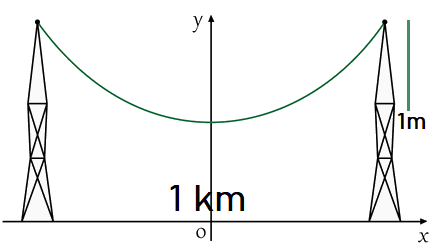
\includegraphics[width=0.3\textwidth]{catenary}
%    \end{figure*}
%
%    Solution is given by the equation
%    \[
%        \lambda \cdot \cosh\Bigl(\frac{500}{\lambda}\Bigr) - \lambda - 1 = 0
%    \]
%    Solve for $\lambda$, which can be used to compute the length of the cable
%    ($\lambda$ here is the radius of curvature at apex).
%    So, we want to find the root of this equation.
%    This is difficult to solve analytically, so we can find 
%    an approximation of $\lambda$.
%\end{example}

%\subsection{Bisection method}
%For cases like
%\begin{align*}
%    f(x) &= 12 x^2 - 5x - 2 = 0\\
%    &=(4x + 1)(3x - 2q)
%\end{align*}
%we can solve using the formula, and get $x_1 = -\frac{1}{4},\ x_2 = \frac{2}{3}$.
%But this does not work for a more complex problem, e.g.
%$f(x) = \log(3 + x^4) + 3\sin(x) = 0$.

%\begin{itemize}
%    \item {
%        We need to find an algorithm that gives a \textit{robust}
%        root localization (has to work for any nonlinear function).
%    }
%    \item {
%        We don't know how many roots there are. The algorithm should find at least one root per search.
%    }
%\end{itemize}


\pagebreak
\section{Nonlinear equations}
Linear equations can be represented by a matrix. On the other hand, nonlinear equations can't.
Nonlinear equations are about finding roots. They appear in many applications.

\begin{example}
    If we want to solve
    \[ x^2 + 3x + 7 = \log(x) \]
    If we bring it all to one side, then we have to find the root of a function.
    \[ x^2 + 3x + 7 - \log(x) = 0 \]
    Unfortunately, non-linear equations are difficult to solve analytically.
    We can usually approximate the solution by using iterative methods.
\end{example}

\subsection{Bisection method}
\begin{theorem}
    Let $f \in \operatorname{C}([a, b])$ ($f(x)$ is continuous on $[a, b]$)
    with $f(a) \cdot f(b) < 0$ (i.e. $f$ has different signs on its ends).
    Then, by continuity, there exists $r \in (a, b)$, such that
    $f(r) = 0$.
\end{theorem}
\begin{remark}
    Actually, this theorem tells that any point between $f(a)$ and $f(b)$ will be achieved.
\end{remark}

\textbf{Idea of the bisection method:}
\begin{enumerate}
    \item {
        Bisection of $[a, b]$ into $[a, c] \cup [c, b]$, i.e.
        into two subintervals, $a < c < b$.
    }
    \item {
        If $f(c) = 0$, then $r = c$, we have found the solution.
    }
    \item {
        If $f(c) \cdot f(a) < 0$, then continue with $[a, c]$.
    }
    \item {
        If $f(c) \cdot f(b) < 0$, continue with $[c, b]$.
    }
\end{enumerate}
\begin{remark}
    When $f(a) \cdot f(b) > 0$, $f$ may or may not have a root on $[a, b]$ ---
    we cannot say for sure.
\end{remark}
\begin{remark}
    This algorithm will only find one root, not all.
\end{remark}

\textbf{The method in short:}

Producing a sequence of intervals $[a_i, b_i]$ such that a root $r$ is inside these intervals.
The starting interval is $[a, b] = [a_0, b_0]$.

\begin{theorem}
    The bisection method, when applied to $[a, b]$ and 
    $f \in C^*([a, b])$ with $f(a) \cdot f(b) < 0$ will complete after
    $n$ steps an approximation $c_n$ of root $r$ with error
    \[ \abs{r - c_n} < \frac{b - a}{2^n} \]
\end{theorem}
\begin{remark}
    If we do infinitely many iterations, we will always find the root, because
    \[ \lim_{n \to \infty} \frac{b - a}{2^n} = 0 \]
\end{remark}
\begin{proof}
    At every step, the length of the interval where the root is located
    is divided into two. We can use induction to prove the above-mentioned error formula.
\end{proof}

\begin{example}
    Let $[a, b] = [0, 1]$. How many iterations are needed to decrease the error
    below $2^{-20} \approx 10^{-6}$?

    We need to find an $n \in \mathbb{N}$, such that our error estimate
    is less than what we want:
    \begin{align*}
        &
        \frac{b - a}{2^n} < 2^{-20} \Longleftrightarrow
        \frac{b - a}{2^{-20}} < 2^n \Longleftrightarrow
        \log_2\Bigl(\frac{b - a}{2^{-20}}\Bigr) 
        \overset{\text{$\log_2$ is strictly increasing}}{<} \log(2^n) = n
        \\&
        \log_2\Bigl(\frac{1}{2^{-20}}\Bigr) < n \Longleftrightarrow
        \log_{2}(1) - \log_{2}(2^{-20}) < n \Longleftrightarrow
        0 - (-20) < n \Longleftrightarrow 20 < n
    \end{align*}
\end{example}
\begin{remark}
    The bisection method has a slow convergence.
    For every iteration step we get a \textit{binary} digit as our accuracy increase.
    Recall that for approximating $\cos(x)$ by Taylor polynomial,
    we get 2 decimal digits per term of the polynomial. 
\end{remark}

\subsection{Newton method}

\begin{definition}
    Suppose that the sequence $\{x_n\}$ converges as $n \to \infty$.
    Then the sequence:
    \begin{enumerate}[label=\alph*)]
        \item {
            converges \textit{linearly} to $r$, if 
            there exists such an $M \in (0, 1)$, such that
            \[ \lim_{n \to \infty} \frac{\abs{x_{n + 1} - r}}{\abs{x_{n} - r}} = M \]
            \begin{example}
                For bisection method $M = \frac{1}{2}$.
            \end{example}
        }
        \item {
            converges \textit{super-linearly} to $r$, if
            \[ \lim_{n \to \infty} \frac{\abs{x_{n + 1} - r}}{\abs{x_{n} - r}} = 0 \]
        }
        \item {
            converges \textit{sub-linearly} to $r$, if
            \[ \lim_{n \to \infty} \frac{\abs{x_{n + 1} - r}}{\abs{x_{n} - r}} = 1 \]
            (i.e. at some point the error decrease rate stagnates).
        }
        \item {
            converges \textit{with order $q > 1$}, if there exists $M > 0$, such that
            \[ \lim_{n \to \infty} \frac{\abs{x_{n + 1} - r}}{\abs{x_{n} - r}^q} < M \]
            If $q = 2$, the convergence is called \textit{quadratic},
            if $q = 3$ --- cubic.
        }
    \end{enumerate}
\end{definition}

\begin{definition}[Newton method]
    Let $f \in \operatorname{C}^1([a, b])$. Then at every 
    $x_0 \in (a, b)$ there exists a tangent to the graph of $f$.
    The tangent equation at $x_0$ can be written as follows:
    \begin{align*}
        &
        t(x) = f(x_0) + f'(x_0)(x - x_0)
        \\&
        \frac{t(x) - f(x_0)}{x - x_0} = f'(x_0)
    \end{align*}
    If we recall, the tangent at $x_0$ is the first order Taylor polynomial of $f(x)$
    with $t(x_0) = f(x_0),\ t'(x) = f'(x_0)$.
    \pagebreak
    \begin{figure*}[h]
        \centering
        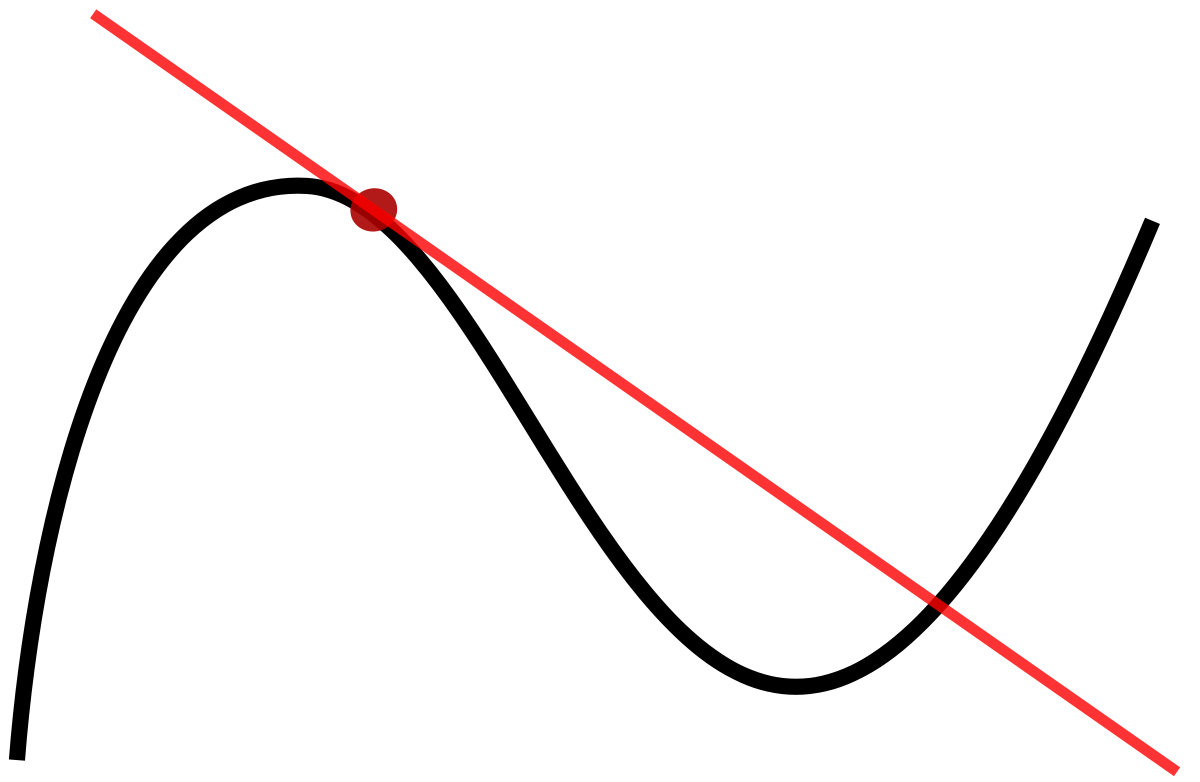
\includegraphics[width=0.3\textwidth]{tangent}
    \end{figure*}

    We use the tangent $t(x)$ as an approximation to $f(x)$,
    and we can find the root of $t(x)$ easily, as it's a linear funciton:
    \[
        0 = t(x_1) = f(x_0) + f'(x_0)(x_1 - x_0) \Longleftrightarrow
        x_1 = x_0 - \frac{f(x_0)}{f'(x_0)}
    \]

    Continuing yields the Newton sequence (Newton–Raphson iteration):
    \[ x_{n + 1} = x_n - \frac{f(x_n)}{f'(x_n)},\ x_0 = \text{initial guess} \]

    \begin{figure*}[h]
        \centering
        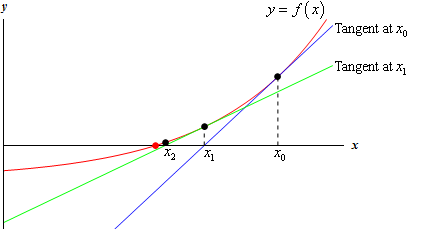
\includegraphics[width=0.5\textwidth]{newton}
    \end{figure*}

    Here we cannot have $f'(x_n) = 0$, since we cannot divide by zero. Therefore,
    it's often a good idea to make sure $f'$ doesn't have roots on the interval
    of search.
\end{definition}
\begin{theorem}
    When the Newton sequence converges, it converges to
    \textbf{a} root of $f$.
\end{theorem}
\begin{theorem}
    Suppose we have a function $f \in \operatorname{C}^2([a, b])$, such that:
    \begin{enumerate}
        \item {
            $f(a) \cdot f(b) < 0$ (there's a sign switch).
        }
        \item {
            $f$ has no critical points in $(a, b)$ (i.e. $f'(x) \ne 0$ for $x \in (a, b)$).
        }
        \item {
            $f''$ exists, is continuous and either $f'' > 0$
            or $f'' < 0$ on the whole $(a, b)$.
            I.e., $f$ is either concave down or concave up.
        }
    \end{enumerate}
    Then $f(x) = 0$ has \textit{exactly one} solution $r$. 
    The Newton sequence always converges to $r$.

    For $n \to \infty$, when the initial guess should be chosen according to:
    \begin{itemize}
        \item {
            If $f(a) < 0$, $f'' < 0$ or $f(a) > 0, f'' > 0$
            then $x_0 \in [a, r]$, e.g. $x_0 = a$.
        }
        \item {
            If $f(a) < 0$, $f'' > 0$ or $f(a) > 0$, $f'' < 0$ then
            $x_0 \in [r, b]$, e.g. $x_0 = b$.
        }
    \end{itemize}
    (If we chose an initial guess on the wrong side of the graph, then 
    the Newton method may diverge outside the domain area of  $(a, b)$ --- we don't want that.)

    In any case we have the estimate
    \[ \abs{x_n - r} < \frac{f(x_n)}{\min_{[a, b]} \abs{f'(x)}} \]
\end{theorem}

Problems with the Newton method:
\begin{enumerate}
    \item {
        The runaway problem: the Newton method may start stepping in the wrong side.
        \begin{figure*}[h]
            \centering
            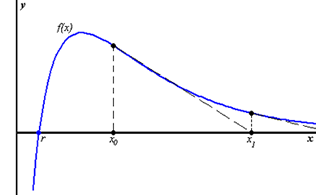
\includegraphics[width=0.5\textwidth]{runaway}
        \end{figure*}
    }
    \item {
        If we have a flat point, we don't know in which direction to go:
        \begin{figure*}[h]
            \centering
            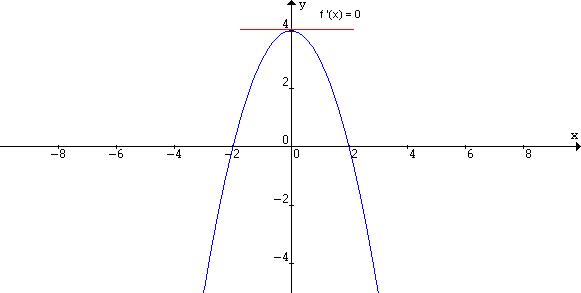
\includegraphics[width=0.5\textwidth]{flat_point}
        \end{figure*}
    }
    \item {
        Sometimes the Newton method can jump infinitely between two points in a cycle
        without ever converging.
        \begin{figure*}[h]
            \centering
            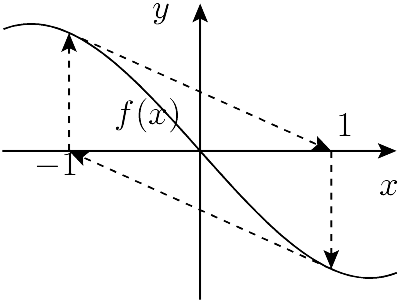
\includegraphics[width=0.5\textwidth]{newton_cycle}
        \end{figure*}
    }
\end{enumerate}
\pagebreak
\begin{theorem}
    If $f : [a, b] \to \mathbb{R}$ fullfills:
    \begin{enumerate}
        \item {
            $f(a) \cdot f(b) < 0$.
        }
        \item {
            $f$ has no critical points in $(a, b)$.
        }
        \item {
            $f''$ exists and is continuous ($f \in \operatorname{C}^2([a, b])$)
            and $x_0$ is \textit{``close enough''} (not a mathematical term)
            to the root $r$.
        }
    \end{enumerate}
    Then the Newton sequence converges quadratically.
\end{theorem}
\begin{proof}
    We have to show that
    $\abs{x_{n + 1} - r} \le M \abs{x_n - r}^2$ as $n \to \infty$.
    By Taylor series approximation,
    \[ 
        f(x) = f(x_n) + f'(x_n)(x - x_n) + \frac{1}{2} f''(\xi_n)(x - x_n)^2 
        \text{, where } \xi_n \in (x, x_n)
    \]
    Since $r$ is a root of $f$, when we put $x = r$, we get
    \[
        0 = f(r) = f(x_n) + f'(x_n)(r - x_n) + \frac{1}{2} f''(\xi_n)(r - x_n)^2
    \]
    Let's divide both sides by $f'(x_n)$ and rearrange the terms:
    \begin{align*}
        &\frac{f(x_n)}{f'(x_n)} +
        \frac{f'(x_n)}{f'(x_n)} (r - x_n) = -\frac{f''(\xi_n)}{2 f'(x_n)}(r-x_n)^2
        \\&\Longleftrightarrow (r - x_{n+1}) = -\frac{f''(\xi_n)}{2 f'(x_n)} (r - x_n)^2
        \quad \Bigl(x_{n+1} = x_n - \frac{f(x_n)}{f'(x_n)}\Bigr)
        \\&\implies \abs{r - x_{n+1}} = \abs{\frac{f''(\xi_n)}{2f'(x_n)}} \abs{r - x_n}^2
    \end{align*}
    Let
    \[ M \coloneqq \sup_{x_n,\, \xi_n} \abs{\frac{f''(\xi_n)}{2f'(x_n)}} \]
    The supremum will be finite, because $x_n$ and $\xi_n$ are both
    inside bounded intervals.

    Then $\abs{r - x_{n + 1}} \le M \abs{r - x_n}^2$.
\end{proof}
\begin{remark}
    We need $x_0$ to be close enough to make sure the Newton method
    doesn't go outside the domain $[a, b]$.
\end{remark}

\subsection{Modifications of the Newton method}
\subsubsection{Modified Newton method}
As we remember, in the usual Newton method
\[ x_{n+1} = x_n - \frac{f(x_n)}{f'(x_n)} \]
If $f'(x_n)$ doesn't change much anymore from $n$ to $n + 1$, we can fix it to
$f'(x_m)$ with some fixed $m \le n$. Then our new formula for $x_{n+1}$ is
\[ x_{n + 1} = x_n - \frac{f(x_n)}{f'(x_m)} \]
We avoid futher evaluations of $f'(x)$ which saves computational resources.

\subsubsection{Secant method}
Newton's method needs derivatives. 
We can approximate the derivatives by secants (also called a difference quotient):

\[
    f'(x) = \lim_{h \to 0} \frac{f(x + h) - f(x)}{h} \implies
    f'(x) \approx \frac{f(x + h) - f(x)}{h} \text{ for small $h$}
\]
For the Secant method, we let $x_n \coloneqq x_n,\ h \coloneqq x_{n - 1} - x_{n}$.
\[ f'(x_n) \approx \frac{f(x_{n - 1}) - f(x_n)}{x_{n - 1} - x_{n}} \]
Substitution into Newton method gives us
\[ x_{n + 1} = x_{n} - \frac{f(x_n) (x_{n - 1} - x_{n})}{f(x_{n - 1}) - f(x)} \]

The Secant method converges slower than the Newton method, but it's easier to compute.

\begin{theorem}
    If $f \in \operatorname{C}^2([a, b])$
    and $r \in (a, b),\ f(r) = 0,\ f'(r) \ne 0$
    and 
    \[ x_{n + 1} = x_n - \frac{f(x_n) (x_{n-1} - x_n)}{f(x_{n - 1} - f(x_n))} \]
    Then there exists a $\delta > 0$, such that for every $x_1, x_0$, such that
    $\abs{r - x_1} < \delta$, $\abs{r - x_0} < \delta$, we'll have
    \begin{enumerate}
        \item {
            $\lim_{n \to \infty} \abs{x_n - r} = 0$ (the sequence converges)
        }
        \item {
            $\abs{r - x_{n + 1}} \le M \abs{r - x_n}^\alpha$
            with $\alpha = \frac{1 + \sqrt{5}}{2} \approx 1.618$
            (the sequence converges with order of golden ratio).
        }
    \end{enumerate}
\end{theorem}
\begin{example}
    \[ f(x) = x^5 - 3x + 1 = 0,\ f'(x) = 5x^4 + 3 \]
    Newton method:
    \begin{align*}
        &x_0 = 0,\ f(0) = 1,\ f'(0) = 3
        \\&
        x_1 = x_0 = \frac{f(x_0)}{f'(x_0)} = 0 - \frac{1}{3} = -\frac{1}{3}
    \end{align*}

    Secant method:
    \begin{align*}
        &x_0 = 1,\ x_1 = \frac{1}{2}
        \\&
        x_2 = \frac{1}{2} - \frac{f(1/2)(1 - 1/2)}{f(1) - f(1/2)} = \dots
    \end{align*}
\end{example}

Summary:
{
\scriptsize
\[\begin{array}{c|c|c|c|c|c}
    & \text{\#initials} & \text{Regularity of $f$} & \text{Convergence} & \text{Root between points} & \text{Function calls per iteration}
    \\\hline
    \text{Bisection} & \text{2 ($a$, $b$)} & \operatorname{C}([a, b]) & \text{linear} & \text{Yes} & 1
    \\\hline
    \text{Newton} & \text{1 ($x_0$)} & \operatorname{C^2}([a, b]) &
    \text{quadratic} & \text{No} & 2
    \\\hline
    \text{Secant} & \text{2 ($x_0$, $x_1$)} & \operatorname{C^2}([a, b]) &
    \text{superlinear/order $\alpha = 1.618$} & \text{No} & 1
\end{array}
\]
}
\begin{theorem}[Simple approximation theorem]
    $f: E \to \overline{\mathbb{R}}$ is measurable if and only if 
    there exists a sequence of simple functions $\varphi_n : E \to \mathbb{R}$,
    such that $\varphi_n \to f$ pointwise on $E$, and $\abs{\varphi_n} \le \abs{f}$
    on $E$ for all $n$.

    (If $f \ge 0$, then $\{\varphi_n\}$ can be chosen to be increasing.)
\end{theorem}
\begin{remark}
    In the simple approximation lemma, functions 
    $\varphi_\varepsilon$ and $\psi_\varepsilon$ sandwich the function $f$,
    and\\ $0 \le \psi_\varepsilon - \varphi_\varepsilon < \varepsilon$, therefore, 
    at every point they both differ from $f$ by no more than $\varepsilon$.
    If we could choose a sequence of $\varepsilon$'s that converges to 0,
    we would get uniform convergence.

    Unfortunately, we can't apply the lemma directly, because we needed the function $f$ to be bounded.
    That's why we're not getting uniform convergence.
\end{remark}
\begin{proof}
    \begin{enumerate}
        \item {
            $\impliedby$. We have a sequence of simple (and thus measurable) functions $\{\varphi_n\}$,
            therefore, their limit is also measurable.
        }
        \item {
            $\implies$.
            \begin{enumerate}[label={(\arabic*)}]
                \item {
                    Let's express $f = f^+ - f^-$, where $f^+ = \max\{f, 0\}$ and $f^- = \min\{f, 0\}$.
                    Let's prove the theorem for both $f^+$ and $f^-$.
                    Without the loss of generality, assume that $f \ge 0$.
                }
                \item {
                    To use the simple approximation lemma, we have to make the function bounded.
                    Define $f_n \coloneqq \min\{f, 2^n\}$.
                    Take $\varphi_n$ as the lower simple approximation of $f_n$,
                    according to the simple approximation lemma, with $\varepsilon = \frac{1}{2^n}$.

                    Then $\varphi_n \to f$ pointwise. Moreover, $\{\varphi_n\}$ 
                    are increasing (because we bound it with $2^n$, and because when we 
                    go from $n$ to $n + 1$, every interval in the proof of SAL is split into two).
                }
                \item {
                    Do the same for $f^-$ and add the sequences for $f^+$ and $f^-$ together.
                    Since $\abs{f} = \max\{\abs{f^+}, \abs{f^-}\}$, the condition
                    of $\abs{\varphi_n} \le \abs{f}$ will hold true. 
                }
            \end{enumerate}
        }
    \end{enumerate}
\end{proof}

\subsection{Egoroff, Lusin, Littlewood's three principles}
Informal statement:
\begin{enumerate}
    \item {
        Every measurable set is \textit{nearly} (not a mathematical term) a finite union of intervals.
    }
    \item {
        Every measurable function is nearly continuous.
    }
    \item {
        Every pointwise convergent sequence of measurable functions is nearly uniform convergent.
    }
\end{enumerate}
\begin{theorem}[Egoroff's theorem]
    Assume that $m(E) < \infty$, 
    $f_n : E \to \overline{\mathbb{R}}$ --- measurable, $f_n \to f$
    pointwise almost everywhere on $E$, where $f : E \to \mathbb{R}$.
    Then for any $\varepsilon > 0$ there exists a closed subset
    $F \subset E$, such $m(E \setminus F) < \varepsilon$ and $f_n \to f$
    uniformly on $f$.
\end{theorem}
\begin{remark}
    It is crucial that $f$ is from $E$ to $\mathbb{R}$, not $\mathbb{\overline{R}}$,
    otherwise we wouldn't get uniform convergence.
\end{remark}
\begin{proof}
    $\abs{f} < \infty \implies \abs{f - f_k}$ is defined for all $x \in E$
    (starting from some $k$).

    Let's also throw out the subset of measure $E$, on which $f_n \not\to f$.

    \begin{enumerate}
        \item {
            Fix $\eta > 0$.
            \[ E_n \coloneqq \{ x \in E \mid \abs{f(x) - f_k(x)} < \eta,\ \forall k \ge n \} \]
            Each set $E_n$ is measurable, because $\abs{f(x) - f_k(x)}$ is measurable,
            and $E_n$ is the countable intersection of preimages of $[0, \eta)$ for all $k$.
            We can also note that $\{E_n\}$ is ascending.
            
            Also, $ \cup_{n=1}^\infty E_n = E $.
            That's follows from pointwise convergence. If we take any point from the set $E$,
            eventually it will be contained in some $E_n$, because for a given point $x$
            the difference $\abs{f(x) - f_k(x)}$ has to converge to 0. 
            Therefore,
            \[
                \lim_{n \to \infty} m(E_n) = m(E)
            \]
            Then there exists $N \in \mathbb{N}$, such that 
            $m(E \setminus E_n) < \varepsilon$ for every $\varepsilon > 0$.
        }
        \item {
            Now let's take such $N$ for $\eta_n = \frac{1}{n}$,
            $\varepsilon_n = \frac{\varepsilon}{2^{n + 1}}$.

            Take $E_n = E_N$, where $E_N$ is from step 1
            for $\eta = \eta_n$ and $\varepsilon = \varepsilon_n$.

            Take $A = \cap_{n=1}^\infty E_n$. Then
            $f_n \to f$ uniformly on $A$. On the other hand, 
            $A$ is measurable as a countable union of measurable sets.

            Let's estimate the measure of $A$.
            \[ m(E \setminus A) = m\Bigl(
                \bigcup_{k=1}^\infty (E \setminus E_n)
            \Bigr) \le
            \sum_{n=1}^\infty m(E \setminus E_n) \le
            \sum_{n=1}^\infty \frac{\varepsilon}{2^{n+1}} = \frac{\varepsilon}{2}
            \]
            But $A$ may be non-closed, so we can't just assign $F$ to $A$.
            Therefore, we have to approximate $A$ by closed sets.
        }
        \item {
            Take $F \subset A$, so that $F$ is closed and
            $m(A \subset F) < \frac{\varepsilon}{2}$.
            We \hyperref[the:lebesgueMeasurableConditions]{have proved} that such an $F$ exists if $A$ is measurable.
        }
    \end{enumerate}
\end{proof}

\begin{theorem}[Lusin's theorem]
    $f : E \to \mathbb{R}$ --- measurable. Then for every
    $\varepsilon > 0$ there exists a continuous function
    $g : \mathbb{R} \to \mathbb{R}$ and a closed set $F \subset E$, 
    such that $f = g$ on $F$ and $m(E \setminus F) < \varepsilon$.
\end{theorem}
\begin{proof}
    \textit{Main idea}: uniform limit of continuous functions is continuous,
    then apply Egoroff's theorem.

    The proof is gonna be split into two parts:
    \begin{enumerate}
        \item {
            Find a closed $F$ on which $f$ is continuous (in induced topology).
        }
        \item {
            Extend $f|_F$ to a continuous function $g$.
            We have briefly discussed how to do this:
            the complement of a closed set $F$ is an open set, 
            and thus a disjoint union of open intervals. On every such
            open interval we can connect the graph of $f$
            with a straight line. There's some work to be done, because
            there can be an infinite number of such intervals converging a point,
            but we'll leave it as an exercise.
        }
    \end{enumerate}

    Proof of Part 1:
    \begin{enumerate}
        \item {
            Assume $m(E) < \infty$. (Let's leave $m(E) = \infty$
            as an exercise).
            By simple approximation lemma, there exists a sequence of 
            simple functions $f_n : E \to \mathbb{R}$, such that
            $f_n \to f$ pointwise.
        }
        \item {
            $\forall n$ there exists a closed subset $F_n \subset F$,
            such that $f_n$ is continuous on $F_n$ and
            $m(E \setminus F_n) < \frac{\varepsilon}{2^{n+1}}$.
            
            Proof:
            \[ f_n = \sum_{j=1}^{k_n} c_j \cdot \chi_{E_j} \text{ --- canonical representation} \]
            Each of the sets $E_j$ 
            \hyperref[the:lebesgueMeasurableConditions]{can be approximated}
            by a closed set $G_j$ from the inside (they are measurable from
            \hyperref[def:simpleFunction]{the definition of a simple function}).

            Put $F_n \coloneqq \cup G_j$. It's a finite union, therefore $F_n$ is closed.

            $f_n$ is constant on each of $G_j$, as $G_j \subset E_j$.
            A preimage of an open set for $f$ was a union of several $E_j$'s.
            If we now restrict $f$ onto $\cup G_j$, the preimage of an open set
            will be a union of several $G_j$'s. What we have to prove that 
            $G_j$'s are open in the induced topogy on $F_n$ --- that's 
            true because $G_j$'s are closed in $\mathbb{R}$ and disjoint.
        }
        \item {
            By Egoroff's theorem, there exists a closed $F_0 \subset E$, 
            such that $m(E \setminus F_0) < \frac{\varepsilon}{2}$ and 
            $f_n \to f$ uniformly.
            Now take $F \coloneqq \cap_{n=0}^\infty F_n$. The intersection of closed sets 
            is closed. 
            By construction, $f_n$ is continuous on $F$, as $F_n \subset F$.
            Since $f_n \to f$ uniformly on $F$ (as $F_0 \subset F$),
            $f$ is continuous on $F$.
            Let's now estimate the measure of $E \setminus F$:
            \[
                m(E \setminus F) < \frac{\varepsilon}{2} + 
                \sum_{n=1}^\infty \frac{\varepsilon}{2^{n+1}} = \varepsilon
            \]
        }
    \end{enumerate}
\end{proof}
\begin{remark}
    If $m(E) = \infty$, we can split $\mathbb{R}$ into intervals with finite length.
    Then use the finite case we've just proved for each of those intervals,
    but choose $\varepsilon_k = \frac{\varepsilon}{2^{k + 1}}$ so that they all sum 
    up to $\varepsilon$ at the end.
\end{remark}

\pagebreak
\section{Lebesgue integral}
\begin{definition}
    Let $\psi : E \to \mathbb{R}$ be simple, $m(E) < \infty$. Let
    \[ \psi = \sum_{n=1}^k a_n \cdot \chi_{E_n} \]
    be the canonical representation of $\psi$. Then define
    \[ \int_E \psi \coloneqq \sum_{n=1}^k a_n \cdot m(E_n) \]
\end{definition}
\begin{remark}
    Notation: if we want to emphasize the measure, we can write
    \[ \int_E \psi = \int_E \psi \,dm = \int_a^b \psi \,dm \text{ (when $E=[a, b]$)} \]
\end{remark}
\begin{remark}
    One can show that if it's not the canonical representation,
    we can still compute the integral by the same formula and get the same result.
\end{remark}

\begin{definition}
    Let $f : E \to \mathbb{R}$ be bounded, $m(E) < \infty$.
    ($f$ is not necessarily measurable).

    The \textit{lower Lebesgue integral} is by definition
    \[ \sup\Bigl\{ \int_E \varphi \mathrel{\Big\vert} \text{ $\varphi$ is simple and $\varphi \le f$ on $E$} \Bigr\} \]
    The \textit{upper Lebesgue integral} is by definition
    \[ \inf\Bigl\{ \int_E \psi \mathrel{\Big\vert} \text{ $\varphi$ is simple and $\varphi \ge f$ on $E$} \Bigr\} \]
    $f$ is \textit{Lebesgue integrable} if the lower Lebesgue integral
    is equal to the upper Lebesgue integral. Then
    \[ \int_E f \coloneqq \text{lower Lebesgue integral} = \text{upper Lebesgue integral} \]
\end{definition}

\begin{theorem}
    $f : [a, b] \to \mathbb{R}$ is bounded and $[a, b]$ is bounded.
    If $f$ is Riemann integrable over $[a, b]$, then 
    $f$ is Lebesgue integrable and both integrals will match.
\end{theorem}
\begin{proof}
    Upper and lower Riemann sums are obtained by simple functions.
\end{proof}
\begin{theorem}
    If $f : E \to \mathbb{R}$ is bounded and \textit{measurable}, 
    $m(E) < \infty$, then $f$ is Lebesgue integrable on $E$.
\end{theorem}
\begin{proof}
    By the simple approximation lemma, for every $n \in \mathbb{N}$
    there exist simple functions $\varphi_n$, $\phi_n$, such that
    $\varphi_n \le f \le \psi_n$ on $E$ and
    $\psi_n - \varphi_n \le \frac{1}{n}$ on $E$.
    \[
        \forall n: 
        (\text{upper Lebesgue integral} - \text{lower Lebesgue integral}) \le
        \int_E \psi_n - \int_E \varphi_n = \int_E (\psi_n - \varphi_n) \le
        \frac{1}{n} m(E) \to 0
    \]
    Here we've used the fact that the difference of two integrals
    is the integral of the difference (which we haven't yet proved).
    However, since we're dealing with simple functions,
    we can prove it by simply rearranging the finite sums.
\end{proof}

Now here's some definitions for the improper case,
i.e. infinite integration limits or functions that converge to infinity.

\begin{definition*}
    $f : E \to \overline{\mathbb{R}}$ is measurable.
    Its support is by definition
    \[ \supp f \coloneqq \{ x \in E \mid f(x) \ne 0 \} \]
    $f$ is of finite support of $m(\supp f) < \infty$.
\end{definition*}
\begin{definition}
    \label{def:definitionThree}
    $f : E \to \overline{\mathbb{R}}$ is measurable, $f \ge 0$. Then
    \[
        \int_E f \coloneqq \sup \Bigl\{
            \int_E h \mathrel{\Big\vert}
            \text{$h$ is bounded, measurable,}\
            m(\supp h) < \infty,\ 0 \le h \le f \text{ on } E
        \Bigr\} 
    \]
    $f$ is Lebesgue integrable over $E$, if $\int_E f < \infty$.
\end{definition}
\begin{definition}
    A measurable function $f : E \to \overline{\mathbb{R}}$
    is Lebesgue measurable over $E$ if 
    $f^+ = \max\{f, 0\}$ and $f^- = \max\{-f, 0\}$ are Lebesgue
    integrable over $E$.
    Then
    \[ \int_E f = \int_E f^+ - \int_E f^- \]
\end{definition}

\begin{definition}
    A function $f: E \to \overline{\mathbb{R}}$
    is \text{integrable} if both $\int_E f^+$ and $\int_E f^-$ are finite.
\end{definition}
\begin{remark}
    If $\int_E f^+$ and $\int_E f^-$ are both infinite, we can't subtract them in the previous
    definition. Therefore, it is not enough to just say that $\int_E f$ has to be finite.
\end{remark}

\begin{theorem}
    \label{the:integralLinearityIntegrable}
    $f, g: E \to \mathbb{R}$ are measurable and integrable. Then 
    for any $\alpha, \beta \in \mathbb{R}$ the linear combination
    $\alpha f + \beta g$ is integrable, and 
    \[ \int_E (\alpha f + \beta g) = \alpha \int_E f + \beta \int_E g \]
\end{theorem}
\begin{theorem}
    \label{the:integralLinearityPositive}
    $f, g: E \to \mathbb{R}$ are measurable and non-negative. Then for any 
    $\alpha, \beta \ge 0$:
    \[ \int_E (\alpha f + \beta g) = \alpha \int_E f + \beta \int_E g \]
\end{theorem}
\begin{proof}
    The proof of these two theorems is technical, we are not gonna prove them here.
    You can read them in the textbook.
    Checking the linearity of simple functions is easy. But the moment 
    we proceed to supremums and infimums it becomes more difficult.
\end{proof}
\begin{remark}
    Why do we need two theorems instead of one? Notice that 
    Theorem~\ref{the:integralLinearityPositive} doesn't 
    require integrability. If $f$ and $g$ are non-negative, then 
    their integrals are non-negative as well, therefore, we can add the two 
    integrals and not worry about cases like $+\infty + (-\infty)$.

    In Theorem~\ref{the:integralLinearityIntegrable}, we require integrability. Therefore, the integrals
    of $f$ and $g$ are both finite, therefore, the right-hand side is well-defined.
    But in $\int_E (\alpha f + \beta g)$ we could indeed have 
    $+\infty + (-\infty)$. But that's not a problem: we will prove later,
    that if a function is integrable, then it's infinite only on a subset
    of measure 0.
\end{remark}

\subsection{Basic properties of Lebesgue integral}
\begin{theorem}[Monotonicity]
    Assume $f, g: E \to \overline{\mathbb{R}}$ are measurable and
    either both integrable or both non-negative. Then 
    if $f \le g$ on $E$, then 
    \[ \int_E f \le \int_E g \]
\end{theorem}
\begin{proof}
    We can use either Theorem~\ref{the:integralLinearityIntegrable} or 
    Theorem~\ref{the:integralLinearityPositive}.
    If $g = f + h$, then $g \ge f \implies h \ge 0 \implies \int_E h \ge 0$.
    But $\int_E g = \int_E f + \int_E h$ by one of those theorems, therefore,
    $\int_E g \ge \int_E f$.
\end{proof}

\begin{proposition}
    $f : E \to \overline{\mathbb{R}}$ is measurable. Then
    $f$ is integrable $\iff$ $\abs{f}$ is integrable.
\end{proposition}
\begin{proof}
    $\abs{f} = f^+ + f^-$.
    \begin{enumerate}
        \item {
            $\implies$.
            If $f$ is integrable, then $\int f^+,\ \int f^- < \infty$ by definition.
            Then
            \[ \int \abs{f} = \int f^+ + \int f^- < \infty \]
        }
        \item {
            $\impliedby$.
            $0 \le f^+ \le \abs{f}$ and $0 \le f^- \le \abs{f}$.
            If $\abs{f}$ is integrable, then, by monotonicity, $f^+$ and $f^-$
            are integrable.
        }
    \end{enumerate}
\end{proof}

\begin{proposition}
    \label{prop:boundedIntegrable}
    $f : E \to \overline{\mathbb{R}}$, $g : E \to \overline{\mathbb{R}}$ --- integrable and
    $g \ge 0$. If $\abs{f} \le g$ on $E$, then $f$ is integrable.
\end{proposition}
\begin{proof}
    If $g$ is integrable, then by monotonicity $\abs{f}$ is integrable,
    then by previous proposition $f$ is integrable.
\end{proof}

\begin{theorem}
    \label{the:integralOnUnion}
    $f: E \to \overline{\mathbb{R}}$ is measurable and either integrable
    or non-negative. If $A, B \subset E$, $A \cap B = \emptyset$;
    $A, B \in \mathcal{M}$, then
    \[ \int_{A \cup B} f = \int_A f + \int_B f \]
\end{theorem}
\begin{proof}
    \[ f\big|_{A \cup B} = f \cdot \chi_A + f \cdot \chi_B = h + g \]
    If $f$ is integrable, then $h$ and $g$ are integrable by previous proposition,
    because $\abs{h} \le \abs{f}$ and $\abs{g} \le \abs{f}$.
    Now apply Theorem~\ref{the:integralLinearityIntegrable}.

    If $f$ is non-negative, then $h, g \ge 0$, apply Theorem~\ref{the:integralLinearityPositive}.
\end{proof}

\begin{proposition}
    If $f : E \to \overline{\mathbb{R}}$ is integrable, then
    \[ \abs{\int_E f} \le \int_E \abs{f} \]
\end{proposition}
\begin{proof}
    \[ \abs{\int_E f} = \abs{\int_E f^+ - \int_E f^-} \le \int_E f^+ + \int_E f^- = \int_E \abs{f} \]
\end{proof}
\begin{theorem}[Chebyshev's inequality]
    $f : E \to \overline{\mathbb{R}}$ --- measurable, $f \ge 0$. Then $\forall \lambda > 0$:
    \[ m(E_\lambda) = m \{ x \in E \mid f(x) \ge \lambda \} \le \frac{1}{\lambda} \int_E f \]
\end{theorem}
\begin{proof}
    Put $h \coloneqq \lambda \cdot \chi_{E_\lambda}$. Since
    $h$ is a simple function,
    \[ \int_{E_\lambda} h = \lambda \cdot m(E_\lambda) \]
    Therefore, it is enough to prove that
    \[ \int_{E_\lambda} h  \le \int_E f \]
    But $h \le f \big|_{E_\lambda}$,
    because on $E_\lambda$ we have $h = \lambda$ and $f \ge \lambda$. Therefore, by monotonicity, 
    \[ \int_{E_\lambda} h \le \int_{E_\lambda} f \le \int_{E} f \]
\end{proof}

\subsubsection*{Applications of the Chebyshev's inequality:}
\begin{proposition}
    $f : E \to \overline{\mathbb{R}}$ is measurable, $f \ge 0$.
    Then \[ \int_E f = 0 \iff f = 0 \text{ almost everywhere on } \mathbb{R} \]
\end{proposition}
\begin{proof}\mbox{}
    \begin{enumerate}
        \item {
            $\implies$.

            If $\int_E f = 0$, then by Chebyshev's inequality,
            \[ m(E_n) = m\Bigl\{x \in E \mathrel{\Big\vert} f(x) \ge \frac{1}{n} \Bigr\}  \le n \int_E f = 0 \]
            The sequence $\{E_n\}$ is ascending. Since the measure of each one of them
            is equal to zero, then, by \hyperref[the:continuityOfMeasure]{continuity of measure},
            $m(\cup_{n=1}^\infty E_n) = m\{x \in E \mid f(x) > 0 \} = 0$.
        }
        \item {
            $\impliedby$. Follows from Definition~\ref{def:definitionThree}.
        }
    \end{enumerate}
\end{proof}

\begin{proposition}
    If $f: E \to \overline{\mathbb{R}}$ is integrable, then $f$ is finite
    almost everywhere on $E$.
\end{proposition}
\begin{proof}
    Without the loss of generality, assume that $f \ge 0$
    (otherwise, prove separately for $f^+$ and $f^-$).
    \[ 
        m\{x \in E \mid f(x) = \infty \} \le m\{x \in E \mid f(x) \ge n \} 
        \overset{\text{Chebyshev's inequality}}{\le} \frac{1}{n} \int_E f 
        \underset{n \to \infty}{\longrightarrow} 0
    \]
    Here we've used that $\int_E f$ is finite, because $f$ is integrable.
\end{proof}

\subsection{Convergence theorems}
\begin{proposition}
    \label{prop:integralUniformLimit}
    $f_n : E \to \overline{\mathbb{R}}$ --- measurable, integrable, $m(E) < \infty$. If $f_n \to f$ uniformly and
    $f$ is bounded on $E$, then 
    \[ \lim_{n \to \infty} \int_E f_n = \int_E f \] 
\end{proposition}
\begin{proof}
    $f$ is measurable (as a pointwise limit). Therefore, $\int_E f$ exists.
    For any $\varepsilon > 0$, choose $N > 0$, such that
    \[
        \abs{f - f_n} < \frac{\varepsilon}{m(E)}, \quad \forall n \ge N
    \]
    Then
    \[
        \abs{\int_E f - \int_E f_n} = \abs{\int_E(f - f_n)} \le
        \int_E \abs{f - f_n} < \frac{\varepsilon}{m(E)} \cdot m(E) = \varepsilon
    \]
\end{proof}

\begin{remark}
    This proposition does not hold for pointwise convergence.
\end{remark}
\begin{example}[1]
    $E = (0, 1],\ f_n \coloneqq n \cdot \chi_{(0, 1/n)}$.
    Then $f_n \to 0$ pointwise. But:
    \[ \int_E f_n = 1 \quad \int_E f = 0 \]
\end{example}
\begin{example}[2]
    $E = \mathbb{R},\ f_n = \chi_{[n, n + 1]}$.
    If we choose an $x$, then for any $n > x$
    this interval will be to the right of $x$, and thus $f_n(x) = 0$.
    Therefore, $f_n \to 0$ pointwise. But:
    \[ \int_E f_n = 1 \quad \int_E f = 0 \]
\end{example}

\begin{theorem}[Bounded convergence theorem]
    $f_n : E \to \overline{\mathbb{R}}$ --- measurable, $m(E) < \infty$.
    Assume that there exists an $M > 0$, such that $\abs{f_n} < M$ on $E$ for all $n$.
    Then if $f_n \to f$ pointwise on $E$, then 
    \[ \lim_{n \to \infty} \int_E f_n = \int_E f \]
\end{theorem}
\begin{remark}
    If we look at the two examples stated earlier as a movie about a function,
    with frames $f_n$, then we can see how the ``mass'' of a function \textit{(not formal)} is moving.
    In the first example, the ``mass'' of the function was escaping vertically. Here
    it's prevented by $\abs{f_n} < M$. In the second example, the ``mass''
    was escaping horizontally. Here it's prevented by $m(E) < \infty$.
\end{remark}
\begin{proof}
    We're gonna use Egoroff's theorem.
    \begin{enumerate}
        \item {
            $f$ is measurable (as a pointwise limit). 
            $\abs{f} \le M$.
        }
        \item {
            For any $\varepsilon > 0$, take $A \subset E$, such that
            $m(E \setminus A) < \frac{\varepsilon}{4M}$ and $f_n \to f$
            uniformly on $A$ (by Egoroff's theorem).
            Then, 
            \[
                \abs{\int_E f_n - \int_E f} \le
                \abs{\int_A f_n - \int_A f} +
                \abs{\int_{E \setminus A} f_n - \int_{E \setminus A} f} = (*)
            \]
            Since $f_n \to f$ uniformly on $A$, we have (by Proposition~\ref{prop:integralUniformLimit})
            that $\abs{\int_A f_n - \int_A f} \to 0$ as $n \to \infty$.
            Now,
            \[
                \abs{\int_{E \setminus A} f_n - \int_{E \setminus A} f} \le
                2M \cdot m(E \setminus A) < \frac{\varepsilon}{2}
            \]
            Since we can make the first modulus be smaller than 
            $\frac{\varepsilon}{2}$ by choosing a sufficiently large $n$, 
            we get that
            \[ (*) \le \frac{\varepsilon}{2} + \frac{\varepsilon}{2} = \varepsilon \]
        }
    \end{enumerate}
\end{proof}

\begin{lemma}[Fatou's lemma]
    $f_n : E \to \overline{\mathbb{R}}$ --- measurable, $f_n \ge 0$.
    If $f_n \to f$ pointwise almost everywhere on $E$, then
    \[
        \int f \le \liminf_{n \to \infty} \int_E f_n 
    \]
\end{lemma}
\begin{remark}
    The sequence of integrals may not have a limit, therefore, we have to use
    $\liminf$ in the statement. By definition,
    \[ \liminf_{n \to \infty} a_n = \lim_{k \to \infty} \inf_{n \ge k} a_n \]
    The since $\inf_{n \ge k} a_n$ is a non-decreasing sequence, the limit
    (possibly infinite) always exists.
\end{remark}
\begin{remark}
    If we think in terms of our escape of the mass analogy, the theorem states that mass can escape,
    but can't enter the limit.
\end{remark}
\begin{proof}
    Exclude a set of measure zero (by Egoroff's theorem), now the convergence is pointwise.
    $f \ge 0$ and $f$ is measurable.

    Recall Definition~\ref{def:definitionThree}.
    Take $h : E \to \overline{\mathbb{R}}$ to be any bounded measurable function with 
    $m(\supp h) < \infty$ and $0 \le h \le f$ on $E$, like in that definition.

    Let $M$ be such that $h \le M$ on $E$ (since $h$ is bounded) and $E_0 \coloneqq \supp h$.
    Define $h_n : E \to \mathbb{R}$ by $h_n \coloneqq \min\{h, f_n\}$. Then:
    \begin{enumerate}
        \item {
            $h_n$ is measurable, because both $h$ and $f_n$ are measurable by their
            respective definitions, and $h_n$ is the minimum of two measurable functions.
        }
        \item {
            $0 \le h_n \le M$, because $h \le M$ on $E$.
        }
        \item {
            $\supp h_n \subset E_0$, as $h_n \le h$.
        }
        \item {
            $h_n \to h$ pointwise on $E$. That's because $f_n$ converges to $f$ pointwise
            and $h \le f$. Therefore, at every point, starting from some $n$, 
            Thus, $h$ will be either less than $f_n$ or arbitrarily close to it, if
            $h = f$ at that point. Since $h_n = \min\{f, h\}$ and 
            $\min\{f, h\} \to h$, we get that $h_n \to h$.
        }
    \end{enumerate}
    By Bounded convergence theorem:
    \[ 
        \lim_{n \to \infty} \int_E h_n 
        \overset{\supp h_n \subset E_0}{=} \lim_{n \to \infty} \int_{E_0} h_n
        \overset{\text{BCT}}{=}
        \int_{E_0} h \overset{\supp h = E_0}{=} \int_E h
    \]
    On the other hand,
    \[
        h_n \le f_n \implies \int_E f_n \ge \int_E h_n \implies
        \int_E h \le \liminf_{n \to \infty} \int_E f_n
    \]
    Since $h$ is arbitrary, by Definition~\ref{def:definitionThree},
    \[
        \int_E f \le \liminf_{n \to \infty} \int_E f_n
    \]
\end{proof}

\begin{theorem}[Monotone convergence theorem]
    $f_n : E \to \overline{\mathbb{R}}$, $f_n \ge 0$, measurable.
    The sequence $\{f_n\}$ is increasing on $E$
    ($f_n \ge f_k$ for $n > k$).
    If $f_n \to f$ pointwise almost everywhere on $E$, then 
    \[ \lim_{n \to \infty} \int_E f_n = \int_E f \]
\end{theorem}
\begin{proof}
    \mbox{}
    \begin{enumerate}
        \item {
            From Fatou's lemma,
            \[ \int_E f \le \liminf \int_E f_n \]
        }
        \item {
            \[ f_n \nearrow \implies \int_E f \ge \limsup \int_E f_n \implies
            \text{all three are equal} \]
        }
    \end{enumerate}
\end{proof}

\begin{theorem}[Lebesgue's dominated convergence theorem]
    \label{the:domConv}
    Let $f_n: E \to \overline{\mathbb{R}}$ --- measurable. Let
    $g : E \to \overline{\mathbb{R}}$ be integrable over $E$, $g \ge 0$.
    Assume that $\abs{f_n} \le g$ for all $n$.

    If $f_n \to f$ pointwise almost everywhere on $E$, then $f$ is integrable
    on $E$ and
    \[
        \lim_{n \to \infty} \int_E f_n = \int_E f
    \]
\end{theorem}
\begin{remark}
    Bounded convergence theorem is a special case with
    \[
        g(x) = \begin{cases}
            M,& x \in E\\
            0,& x \not\in E
        \end{cases}
    \]
\end{remark}
\begin{proof}
    The idea of the proof is to apply Fatou's lemma to $g + f$ and $g - f$.
    \begin{enumerate}
        \item {
            Since $\abs{f_n} \le g$, we have $\abs{f} \le g$ almost everywhere on $E$.
            Therefore, $f$ is integrable as we proved \hyperref[prop:boundedIntegrable]{earlier}.
        }
        \item {
            Remove a subset of measure 0 so that $f$ and each $f_n$ are finite on $E$.
            That's possible, because each of the functions $f$ and $f_n$ has an infinite value on a subset of measure 0,
            and the countable union of subsets of measure 0 also has measure 0.
            Now $g \pm f$ and $g \pm f_n$ are well-defined.
        }
        \item {
            Apply Fatou's lemma:
            \begin{enumerate}
                \item {
                    $f_n \to f$, and $g - f_n$ are non-negative due to the dominance by $g$.
                    \[ 
                        \int_E (g - f) \le \liminf \int_E (g - f_n) =
                        \int_E g- \limsup \int_E f_n
                    \]
                    Now we can cancel out $\int_E g$ on both sides, since it's finite. We get that
                    \[
                        \int_E f \ge \limsup \int_E f_N
                    \]
                }
                \item {
                    Apply Fatou's lemma to the sequence of $g + f_n$, which is also 
                    non-negative due to the dominance by $g$:
                    \[
                        \int_E (g + f) \le \liminf\int_E(g + f_n) =
                        \int_E g + \liminf \int_E f_n \implies
                        \int_E f \le \liminf \int_E f_n
                    \]
                }
            \end{enumerate}
            \[
                \text{(a)} + \text{(b)} \implies \int_E f = \lim_{n \to \infty} \int_E f_n
            \]
        }
    \end{enumerate}
\end{proof}

\begin{theorem}[Countable additivity of integration]$ $\\
    $f : E \to \overline{\mathbb{R}}$ --- integrable.
    $\{E_n\}^\infty$ are disjoint measurable subsets of $E$,
    $E = \cup_{1}^\infty E_n$.
    Then
    \[ \int_E f = \sum_{n=1}^\infty \int_{E_n} f \]
\end{theorem}
\begin{proof}
    Let
    $\chi_n \coloneqq \chi_{\cup_1^n E_k},\ f_n \coloneqq f \cdot \chi_n$.
    Then $f_n$ are measurable and $\abs{f_n} \le \abs{f}$ on $E$
    and $f_n \to f$ pointwise on $E$.
    Hence by Lebesgue's dominance convergence theorem (with $g = f$),
    \[
        \int_E f = \lim_{n \to \infty} \int_E f_n \overset{(*)}{=} \sum_1^\infty \int_{E_n} f
    \]
    Here (*) holds true, because the for a finite sum this equality is true by
    applying induction to \hyperref[the:integralOnUnion]{this theorem}, and 
    then we can take the limits.
\end{proof}

\begin{theorem}[Continuity of integration]
    $f : E \to \overline{\mathbb{R}}$ --- integrable.
    \begin{enumerate}
        \item {
            If $\{E_n\}_1^\infty$ --- ascending, each $E_n$ is measurable, then
            \[
                \int\limits_{\cup_1^\infty E_n} f = \lim_{n \to \infty} \int_{E_n} f
            \]
        }
        \item {
            If $\{E_n\}_1^\infty$ --- descending, each $E_n$ is measurable, then
            \[
                \int\limits_{\cap_1^\infty E_n} f = \lim_{n \to \infty} \int_{E_n} f
            \]
        }
    \end{enumerate}
\end{theorem}
\begin{proof}
    We're not gonna give the full proof, just the proof idea.
    We can use the dominated convergence theorem.
    
    In the first case, define $f_n \coloneqq f \cdot \chi_{E_n}$.
    Since it's an ascending sequence, we'll have $f_n \to f$ pointwise on 
    $\cup_1^\infty E_n$.
    Now apply dominated convergence theorem with $g = f$ on $\cup_1^\infty E_n$.

    The second case is analogous, but we'll have to look at the complement.
\end{proof}
\pagebreak
\section{$L^p$-spaces}
\begin{definition}
    $E$ --- measurable, $1 \le p < \infty$.
    $\hat{L}^p(E)$ is the collection of measurable functions
    $f : E \to \overline{\mathbb{R}}$, such that
    $\abs{f}^p$ is integrable over $E$.
\end{definition}
\begin{remark}
    This is the definition $\hat{L}^p(E)$.
    The definition of $L^p(E)$ is almost the same except a small detail, we will fix it later.
\end{remark}
\begin{remark}
    An integrable function has a \textit{finite} integral.
\end{remark}
Properties of $L^p$:
\begin{definition}[Completeness of reals]
    If $\lim_{n, m \to \infty} \abs{a_n - a_m} = 0$, then there exists $a \in \mathbb{R}$, 
    such that $\lim_{n \to \infty} \abs{a_n - a} = 0$.
\end{definition}
\begin{remark}
    An equivalent formulation: 
    if $\{a_n\}_1^\infty$ is a Cauchy sequence, then
    there exists $a \in \mathbb{R}$, such that
    $\lim_{n \to \infty} a_n = a$.
\end{remark}

\begin{itemize}
    \item {
        Completeness of $L^p(E)$:
        if
        \[ \lim_{n, m \to \infty} \int \abs{f_n - f_m}^p = 0 \]
        then there exists $f \in L^p(E)$, such that
        \[ \lim_{n \to \infty} \int_E \abs{f_n - f}^p = 0 \]
        This is Riesz–Fischer theorem.
    }
    \item {
        $L^p$ is a normed linear space with completeness. With completeness, it 
        follows that
        $L^p$ is a Banach space.
    }
    \item {
        $L^p$ is separable: there exists a countable dense subset in $L^p$.
    }
\end{itemize}

\subsection{Normed linear spaces}
We are going to only consider linear spaces over $\mathbb{R}$.

Examples:
\begin{enumerate}
    \item {
        $C[a, b]$ --- the space of all continuous functions on $[a, b]$.
        The sum of two continuous functions is continuous.
        The null vector is $f(x) \equiv 0$.
        We'll leave the full proof as an exercise.
    }
    \item {
        $B[a, b]$ --- the space of all bounded functions on $[a, b]$.
        If we take the sum of two bounded functions, it will be bounded as well.
        Multiplying by a scalar doesn't break the boundedness, either.
    }
    \item {
        \label{prop:sumIsInLp}
        $\hat{L}^p(E)$ --- the space of $f$, such that $\abs{f}^p$ is integrable.
        We need to prove that $f + g \in \hat{L}^p(E)$
        for $f, g \in \hat{L}^p(E)$, i.e. that $\abs{f+g}^p$ is integrable.
        \begin{proof}
            $f$ and $g$ are infinite on a subset of measure 0, therefore, 
            $f + g$ is undefined on a subset of measure 0. Let's consider the case if
            both $f$ and $g$ are finite:
            \[ \abs{f + g}^p \le \bigl(2 \max(\abs{f}, \abs{g})\bigr)^p \le
            2^p \bigl(\abs{f}^p + \abs{g}^p\bigr) \]
            $\abs{f}^p$ and $\abs{g}^p$ are both integrable, therefore, their sum
            is integrable, and if we multiply it by a constant ($2^p$) it's still integrable.
        \end{proof}
    }
\end{enumerate}
\pagebreak
\begin{definition}[Norm]
    $X$ --- linear space. $\norm{\, \cdot \,}$ --- a real-valued function on $X$, such that
    \begin{enumerate}
        \item {
            $\norm{f + g} \le \norm{f} + \norm{g}$
        }
        \item {
            $\norm{\alpha f} = \abs{\alpha} \cdot \norm{f}$.
        }
        \item {
            $\norm{f} \ge 0$ and $\abs{f} = 0$ if and only if $f = \vec{0}$.
        }
    \end{enumerate}
\end{definition}
\begin{remark}
    A norm defines a metric:
    $l(f, g) \coloneqq \abs{f - g}$.
    However, it doesn't work in the other way: we wouldn't get property 3 from a metric.
\end{remark}
Examples:
\begin{enumerate}
    \item {
        $X = C[a, b],\ \norm{f} \coloneqq \max_{x \in [a, b]} \abs{f(x)}$.
    }
    \item {
        $X = B[a, b],\ \norm{f} \coloneqq \sup_{x \in [a, b]} \abs{f(x)}$.
    }
    \item {
        \[
            X = \hat{L}^p(E),\ \norm{f}_p \coloneqq \biggl(\int_E \abs{f}^p\biggr)^{\frac{1}{p}}
        \]
    }
\end{enumerate}
Here we take the root of power $p$, because property 2 (multiplication by scalar)
has to hold.

However, property 3 doesn't hold, because if $f$ is 0 almost everywhere,
then $\norm{f} = 0$, but $f \ne 0$. We can fix this by putting functions that
differ on a subset of measure zero
into a single equivalence class:
$f \sim g$ if $f = g$ almost everywhere.
Now we arrive at the correct definition of $L^p$:
\begin{definition}
    $L^p(E) \coloneqq \hat{L}^p(E) / {\sim }$
\end{definition}
\begin{remark}
    If $X(f) = 0$ for an $f \in \hat{L}^p(E)$,
    then $f$ is non-zero on a subset of measure 0, therefore, it's
    in the same equivalence class as $g \equiv 0$.
\end{remark}
\begin{remark}
    When we write $f \in L^p(E)$, we will imply that we're talking about the corresponding
    equivalence class $[f]$.
\end{remark}

\begin{definition}
    $f : E \to \overline{\mathbb{R}}$ is \textit{essentially bounded}, if
    there exists $M \ge 0$, such that
    $f(x) \le M$ for almost every $x \in E$. $M$ is called an \textit{essential upper bound}.
\end{definition}
\begin{definition}
    $L^\infty(E)$ is the collection of all equivalence classes $[f]$ of 
    measurable functions $f$ that are essentially bounded.

    $\norm{f}_\infty$ is the infimum of all essential upper bounds of $f$.
    It is also called the \text{essential supremum}. 
\end{definition}

\textbf{Remarks:}
\begin{align*}
    &
    \Phi^\intercal \vec{c} = \vec{y}
    \\&
    \Phi^\intercal \in \mathbb{R}^{(m+1) \times (n + 1)},\
    \vec{y} \in \mathbb{R}^{n+1},\
    \vec{c} \in \mathbb{R}^{m+1}
\end{align*}
is an overdetermined system (there are more equations than unknowns), if equations are independent.
Solution to least squares approximation provides the best approximate
solution to this system, with the error
\[
    \sum_{i=0}^n \Bigl(
        \sum_{j=0}^m c_j g_j(x_i) - y_i
    \Bigr)^2
\]

If we use a polynomial basis, we can ask, what is the best order of polynomial
for data that comes from a polynomial function (with observation error).
I.e. we have
\[ p_N(x) = \sum_{i=0}^N a_i x^i \]
without noise and $y = p_N(x) + \varepsilon$ as data with noise $\varepsilon$.

The variance of errors is from statistics:
\begin{align*}
    &
    \sigma_N^2 = \frac{1}{m - N} \sum_{i=0}^m \bigl(y_i - p_N(x_i)\bigr)^2
    \\&
    \sigma_0^2 > \sigma_1^2 > \dots > \sigma_N^2 = \sigma_{N+1}^2 = \dots = 
    \sigma_{m-1}^2
\end{align*}
We increase degree $N$ until $\sigma_N^2 \approx \sigma_{N+1}^2$.
This is polynomial regression.

\subsection{Differentiation and integration}
When analytical computations of derivatives are not possible, we resort to approximations.
\subsubsection{Difference quotients}
From calculus:
\[
    \lim_{h \to 0} \frac{f(x+h) - f(x)}{h} = f'(x)
\]
So, for $h$ small enough we may approximate
\[
    f'(x) \approx \frac{f(x+h) - f(x)}{h} \text{ --- \textbf{forward differencing}}
\]
How large is the error?
Taylor series expansion:
\begin{align*}
    &f(x+h) = f(x) + h \cdot f'(x) + \frac{h^2}{2} f''(\xi) \qquad \xi \in (x, x + h)
    \\&\iff
    f'(x) = \frac{f(x+h) - f(x)}{h} \textcolor{red}{- \frac{h}{2} f''(\xi)}
\end{align*}

Here $-\frac{h}{2} f''(\xi)$ is the exact error, asymptotically it's $\mathcal{O}(n)$.

What happens if we use
\[
    \lim_{h \to 0} \frac{f(x) - f(x-h)}{h} = f'(x) \text{ --- \textbf{backward differencing}}
\]
Error:
\begin{align*}
    &f(x - h) = f(x) - h f'(x) + \frac{h^2}{2} f''(\xi) \qquad \xi \in (x - h, x)
    \\&\iff
    f'(x) = \frac{f(x) - f(x - h)}{h} \textcolor{red}{+ \frac{h}{2} f''(\xi)}
    \\&
    \frac{h}{2} f''(\xi) = \mathcal{O}(h)
\end{align*}
\textit{Same} order as forward differencing.

Now take the two Taylor series expansions and subtract them:
\begin{align*}
    &
    f(x+h) = f(x) + hf'(x) + \frac{h^2}{2} f''(x) + \frac{h^3}{3!} f'''(\xi_1),\quad \xi_1 \in (x, x + h)
    \\&
    f(x-h) = f(x) - hf'(x) + \frac{h^2}{2} f''(x) - \frac{h^3}{3!} f'''(\xi_1),\quad \xi_2 \in (x, x + h)
    \\&
    f(x + h) - f(x - h) = 2h f'(x) + \frac{h^3}{3!} \bigl(f'''(\xi_1) + f'''(\xi_2)\bigr)
    \\&
    \iff f'(x) = \frac{f(x+h) - f(x-h)}{2h} \textcolor{red}{- \frac{h^2}{12} \bigl(f'''(\xi_1) + f'''(\xi_2)\bigr)}
    \\&
    f'(x) \approx \frac{f(x+h) - f(x-h)}{2h} \text{ --- \textbf{central differencing}}
    \\&
    \frac{h^2}{12} \bigl(f'''(\xi_1) + f'''(\xi_2)\bigr) = \mathcal{O}(h^2) \text{ --- error}
\end{align*}

\begin{figure*}[h]
    \centering
    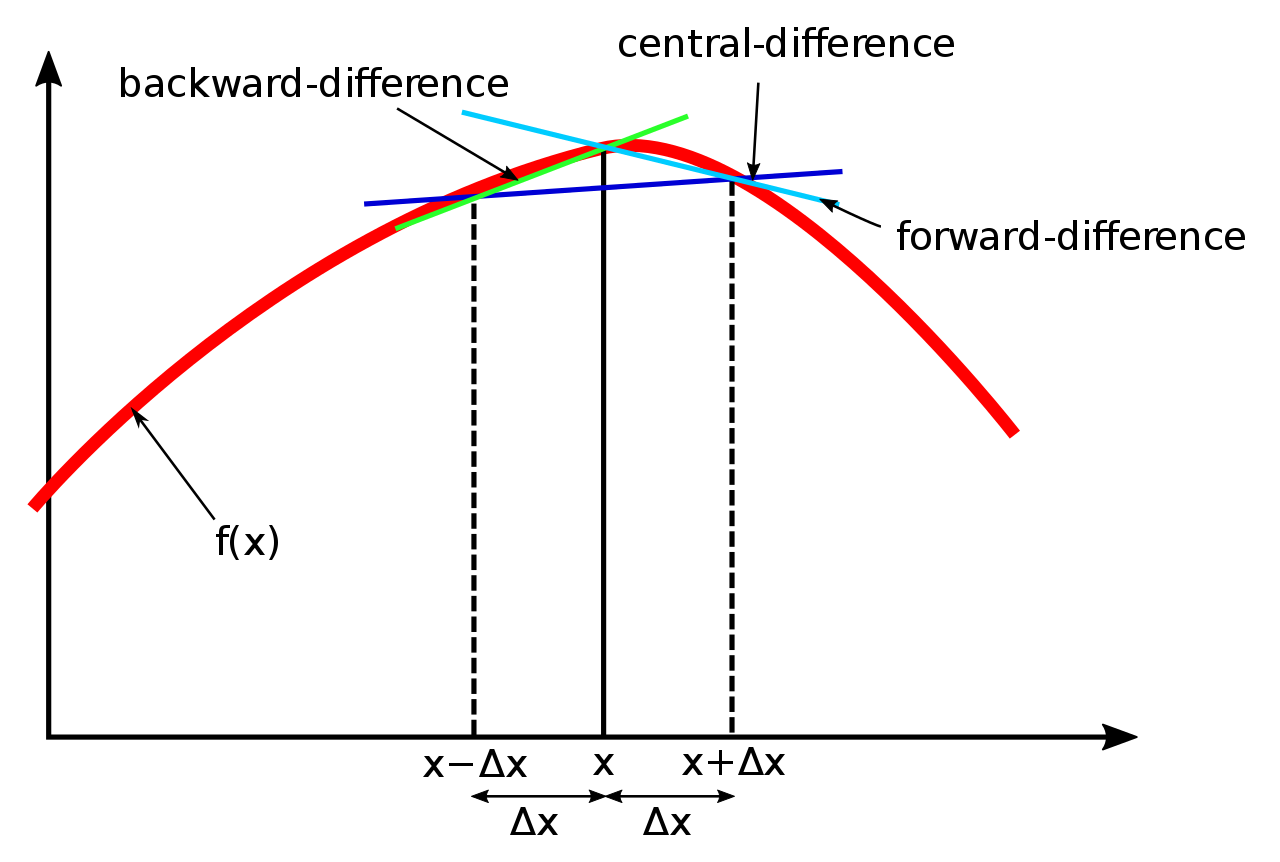
\includegraphics[width=0.7\textwidth]{differences}
\end{figure*}

\subsubsection{Richardson extrapolation}
Approach for producing higher order approximations from lower orrder approximations.

Suppose we have a low order approximation $\varphi(h)$ of a derivative, e.g.
\[
    f'(x) = \varphi(h) + a_1 h + a_2 h^2 + a_3 h^3 + \dots
\]
$\varphi(h)$ may be equal to the first order forward differencing:
\[
    \varphi(h) = \frac{f(x+h) - f(x)}{h}
\]
Alternatively, for central differencing we have:
\[
    \varphi(h) = \frac{f(x+h) - f(x-h)}{2h}
\]

\begin{example}
    For central differencing:
    \[ f'(x) = \varphi(h) + a_2 h^2 + a_4 h^4 + a_6 h^6 + \ldots = \text{(1)} \]
    \textit{Trick:} evaluate for $h = \frac{h}{2}$
    \begin{align*}
        f'(x) &= \varphi\Bigl(\frac{h}{2}\Bigr) + a_2 \Bigl(\frac{h}{2}\Bigr)^2 + 
        a_4 \Bigl(\frac{h}{2}\Bigr)^4 + a_6 \Bigl(\frac{h}{2}\Bigr)^6 + \dots
        \\&
        = \varphi\Bigl(\frac{h}{2}\Bigr) + \frac{a_2}{4} h^2 + \frac{a_4}{16} h^4 + \frac{a_6}{64} h^6 + \ldots
        = \text{(2)}
    \end{align*}
    The idea is to combine (1) and (2) so that the low order terms cancel out.
    \begin{align*}
        &\text{(1)} - 4 \cdot \text{(2)} =
        \varphi(h) - 4 \varphi\Bigl(\frac{h}{2}\Bigr) + a_4\Bigl(1 - \frac{4}{16}\Bigr) h^4 + 
        a_6 \Bigl(1 - \frac{4}{16}\Bigr) h^6 + \dots
        \\&\iff
        -3f'(x) = \varphi(h) - 4 \varphi\Bigl(\frac{h}{2}\Bigr) + a_4 \frac{3}{4} h^4 + a_6 \frac{15}{16} h^6 + \dots
        \\&\iff
        f'(x) = \frac{4 \varphi\bigl(\frac{h}{2}\bigr) - \varphi(h)}{3} \textcolor{red}{- \frac{a_4}{4} h^4 - 
        a_6 \frac{5}{16} h^6 - \dots}
    \end{align*}
    The \textcolor{red}{error} is asymptotically $\mathcal{O}(h^4)$.

    So, the new approximation is
    \[ f'(x) =  \frac{4 \varphi\bigl(\frac{h}{2}\bigr) - \varphi(h)}{3} \]
    In particular, if we substitute $\varphi$ with the
    central differencing, we get
    \[
         f'(x) \approx \frac{f(x-h) - 8f\bigl(x - \frac{h}{2}\bigr) + 
         8f\bigl(x + \frac{h}{2}\bigr) - f(x+h)}{6h}
    \]
\end{example}

The process of halving the step size and cancelling out terms of the error
can be repeated!
We got better approximation at the price of more lower order terms in 
the approximation formula.

For polynomials, the right order Richardson extrapolation will be exact,
as higher order derivatives are zero.

\subsubsection{Higher order derivatives}
Again, we use Taylor series:
\begin{align*}
    &
    f(x+h) = f(x) + hf'(x) + \frac{h^2}{2} f''(x) + \frac{h^3}{3!} f'''(x) 
    + \frac{h^4}{4!} f''''(\xi_1) \quad \xi_1 \in (x, x + h)
    \\&
    f(x - h) = f(x) - hf'(x) + \frac{h^2}{2} f''(x) - \frac{h^3}{3!} f'''(x) 
    + \frac{h^4}{4!} f''''(\xi_2) \quad \xi_2 \in (x - h, x)
\end{align*}
We want to cancel $f'(x)$. For that we can simply add the two series:
\begin{align*}
    &f(x + h) + f(x - h) = 2f(x) + h^2 f''(x) + \frac{1}{4!} h^4 \bigl(
        f''''(\xi_1) + f''''(\xi_2)
    \bigr)
    \\&\iff
    f''(x) = \frac{f(x+h) - 2f(x) + f(x-h)}{h^2}
    \textcolor{red}{- \frac{1}{4!} h^2 \bigl(f''(\xi_1) + f''(\xi_2)\bigr) }
\end{align*}
Here we are using the 3 point stencil (i.e. we need three neighboring points:
$x - h$, $x$, $x+h$), and the weights are $[1, -2, 1]$.
The \textcolor{red}{error} is of order $\mathcal{O}(h^2)$.

Again, Richardson extrapolation can be used to get a better approximation.

\subsubsection*{Summary of numerical derivatives:}
\begin{itemize}
    \item {
        Backward difference quotient, $\mathcal{O}(h)$.
    }
    \item {
        Forward difference quotient, $\mathcal{O}(h)$.
    }
    \item {
        Central difference quotient, $\mathcal{O}(h^2)$.
    }
\end{itemize}
Taylor series expansion is used for error analysus.

Richardson extrapolation: use approximation $\varphi$ for $h$ and $\frac{h}{2}$.
Combine $\varphi(h)$ and $\varphi\bigl(\frac{h}{2}\bigr)$ such that
the low order error terms cancel out, e.g. for central differencing.
\[
    \frac{4 \varphi\bigl(\frac{h}{2}\bigr) - \varphi(h)}{3}
    \text{ is } \mathcal{O}(h^4)
\]

\subsection{Integration/Quadrature rules}
We need numerical integration when anti-derivatives cannot be found easily.

From calculus: assume $f \ge 0$ integrable, $f : [a, b] \to \mathbb{R}$.
Riemann sums:
\begin{enumerate}
    \item {
        Partition $P$ of $[a, b]$. Introduce nodes
        $a = x_0 < x_1 < \dots < x_n = b$ (discretize continuous interval)
        and sub-intervals $[x_i, x_{i+1}]$, for $i = 0, \dots, n - 1$.
        \begin{center}   
            \begin{tikzpicture}
                \begin{axis}[
                    axis x line=left,
                    axis y line=none,
                    axis line style={-{Stealth[scale=1.5]}},
                    xtick={0, 1, 2, 3, 4, 5, 6},
                    xticklabels={$a$, $ $, $ $, $ $, $ $, $ $, $b$},
                    ytick=\empty,
                    xmin=-0.5, xmax=6.5, ymin=0, ymax=1
                ]\end{axis}
            \end{tikzpicture}
        \end{center}
        \begin{figure*}[h]
            \centering
            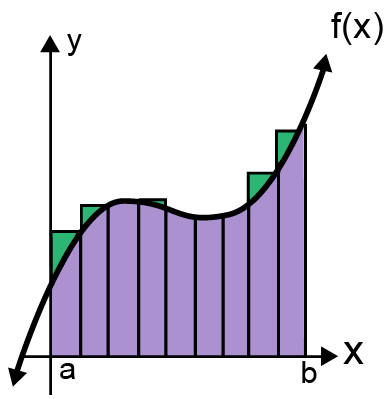
\includegraphics[width=0.25\textwidth]{riemann}
        \end{figure*}
    }
    \item {
        Approximate area under curve by summing up areas of rectangles. \textbf{Riemann sum:}
        \[
            \sum_{i=0}^{n-1} (x_{i+1} - x_i) f(x_i^*) \quad x_i^* \in [x_i, x_{i+1}]
        \]
        Here $x_{i+1} - x_i$ is the width, and $f(x_i^*)$ is the height.
    }   
    \item {
        If $f$ is continuous, then $x_i^*$ may be chosen arbitrarily in $[x_i, x_{i+1}]$.
        Two choices are interesting:
        \begin{enumerate}
            \item {
                $x_i^*$ such that $f(x_i^*) = \min\{ f(x) \mid x_i \le x \le x_{i+1} \} =: m_i$
            }
            \item {
                $x_i^*$ such that $f(x_i^*) = \max\{ f(x) \mid x_i \le x \le x_{i+1} \} =: M_i$
            }
        \end{enumerate}
    }
    \item {
        Then, 
        \begin{align*}
            &
            L(f; P) = \sum_{i=0}^{n-1} (x_{i+1} - x_i) \cdot m_i \text{ --- \textbf{lower sum}}
            \\&
            U(f; P) = \sum_{i=0}^{n-1} (x_{i+1} - x_i) \cdot M_i \text{ --- \textbf{upper sum}}
            \\\implies
            &L(f; P) \le \int_a^b f(x) \,dx \le U(f; P)
        \end{align*}
    }
\end{enumerate}

Some integrations are straight-forward, e.g.:
\[
    f(x) = x^2 \quad \int_a^b f(x)\,dx = \frac{b^3}{3} - \frac{a^3}{3}
\]
But we need numerical methods to find
\[ \int_a^b e^{x^2} \,dx \]
We cannot find an analytical solution consisting of elementary functions. That does not mean
that the function is not integrable!

\begin{theorem}[Minkowski inequality]
    $E$ --- measurable, $1 \le p \le \infty$.
    If $f, g \in L^p(E)$, then 
    $f + g \in L^p$ and 
    $\norm{f + g}_p \le \norm{f}_p + \norm{g}_p$
\end{theorem}
\begin{proof}
    \mbox{}
    \begin{enumerate}[label={Case \arabic*.}]
        \item {
            $p = 1$ --- obvious, $p = \infty$ --- exercise (use essential supremum).
        }
        \item {
            $p \in (1, +\infty)$. Assume that $[f + g] \ne [0]$.
            By part 2 of the previous theorem,
            \begin{align*}
                &\norm{f + g}_p = \int_E (f + g)(f + g)^* = 
                \int_E f (f + g)^* + \int_E g(f+g)^* = \text{(*)}
                \\&
                f \in L^p(E),\ (f+g) \in L^p(E) \implies (f+g)^* \in L^q(E)
                \text{, now use Hölder's inequality:}
                \\&
                \text{(*)} = \norm{f}_p \norm{(f+g)^*}_q +
                \norm{g}_p \norm{(f+g)^*}_q = \norm{f}_p + \norm{g}_p
            \end{align*}
            Note that $f + g \in L^p$, as we proved
            \hyperref[prop:sumIsInLp]{earlier}.
        }
    \end{enumerate}
\end{proof}
\begin{remark}
    There's another way of looking at the Minkowski inequality.
    \begin{center}   
        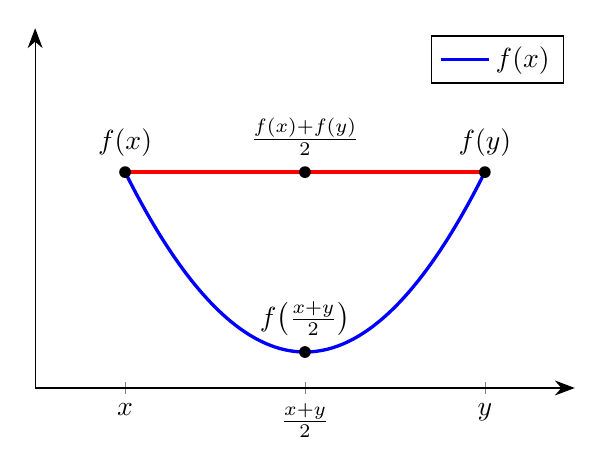
\begin{tikzpicture}
            \begin{axis}[
                axis x line=left,
                axis y line=left,
                axis line style={-{Stealth[scale=1.5]}},
                xtick={0,1,2},
                xticklabels={$x$, $\frac{x+y}{2}$, $y$},
                ytick=\empty,
                xmin=-0.5, xmax=2.5, ymin=-0.2, ymax=1.8,
                unit vector ratio=1 1 1,
                samples=100,
            ]
                \tikzset{graph/.style={very thick, smooth}}
                \tikzset{graph_point/.style={fill,circle,inner sep=1.5pt}}
                \addplot[blue, graph, domain=0:2] {(x - 1)^2};
                \addplot[red, graph, domain=0:2] {1};
                \addlegendentry{$f(x)$}
                \node[graph_point,label={$f(x)$}] at (0, 1){};
                \node[graph_point,label={$\frac{f(x) + f(y)}{2}$}] at (1, 1){};
                \node[graph_point,label={$f\bigl(\frac{x + y}{2}\bigr)$}] at (1, 0){};
                \node[graph_point,label={$f(y)$}] at (2, 1){};
                %\node[graph_point] at (2, 1){$f(y)$};
            \end{axis}
        \end{tikzpicture}
    \end{center}
    A function $f$ is convex if and only if for every $x, y$ we have
    \[
        f\Bigl(\frac{x+y}{2}\Bigr) \le \frac{f(x) + f(y)}{2}
    \]
    Minkowski inequality states that the norm of $f$ is a convex function:
    \[ 
        \norm{f+g}_p \le \norm{f}_p + \norm{g}_p \iff 
        \left\lVert{\frac{f+g}{2}}\right\rVert_p \le \frac{\norm{f}_p + \norm{g}_p}{2}
    \]
    The function $f(x) = x^p$ is only convex for $p \ge 1$, hence we have $p \ge 1$
    in Minkowski inequality statement. (The lecturer forgot the proof here).
\end{remark}

\begin{theorem}[Cauchy-Schwarz inequality]
    If $f, g \in L^2$, then
    \[ \int fg \le \sqrt{\int f^2 \cdot \int g^2} \]
    In linear algebra, we prove that inequality for two vectors in $\mathbb{R}^n$
    and their inner product.
    Therefore, we can define
    \[ \langle f, g \rangle \coloneqq \int fg \]
    Then a lot of properties that hold for vectors will also hold for such an inner product.
\end{theorem}
\begin{proof}
    This is Hölder's inequality for $p = q = 2$.
\end{proof}
\pagebreak
\begin{theorem}
    $m(E) < \infty$. If $1 \le p_1 < p_2 \le \infty$, then
    $L^{p_2}(E) \subset L^{p_1}(E)$.
\end{theorem}
\begin{proof}
    Case $p_2 = \infty$ --- exercise. Now assume that $p_2$ is finite.
    Let's define
    $p \coloneqq \frac{p_2}{p_1} > 1,\ q = \overline{p}$.\\
    If $f \in L^{p_2}(E)$, then
    $ \abs{f}^{p_1} \in L^p(E) $.
    Let's define $g$ as follows:
    \[ g \coloneqq \chi_E \implies \int_E g^q = \int_E 1 = m(E) < \infty \implies
    f \in L^q(E) \]
    Here $\chi_E$ is the characteristic function of $E$.
    Now apply Hölder's inequality:
    \[
        \int_E \abs{f}^{p_1} = \int_E \abs{f}^{p_1} g \le
        \norm{\abs{f}^{p_1}}_p \cdot \norm{g}_q
        \overset{p_1 \cdot p = p_2}{=}
        \Bigl(\int_E \abs{f}^{p_2}\Bigr) \cdot
        \Bigl(\int_E \abs{g}^q\Bigr)^\frac{1}{q} 
        \overset{g^q = g}{=}
        \norm{f}_{p_2}^{p_1} \cdot \bigl(m(E)\bigr)^\frac{1}{q}
    \]
    $\norm{f}_{p_2}$ is finite, as $f \in L^{p_2}(E)$, and $m(E)$ is finite as well,
    therefore, the right side is finite, therefore, $f \in L^{p_1}{E}$.
\end{proof}
\begin{remark}
    
\end{remark}
\begin{proposition}
    We have proved the non-strict inclusion.
    Let's prove that $L^{p_1}(E) \ne L^{p_2}(E)$, i.e.
    that the inclusion is actually strict.
\end{proposition}
\begin{proof}
    Take $E = (0, 1]$, $f(x) = \frac{1}{x^\alpha}$.
    Let's take $\alpha$ such that $\alpha p_2 > 1$ and $\alpha p_1 < 1$
    (which is possible as $p_1 < p_2$).
    Then:
    \begin{align*}
        &\alpha p_2 > 1 \implies \int_E f^{p_2} = 
        \int_0^1 \frac{1}{x^{\alpha p_2}} = \infty \implies
        f \not\in L^{p_2}
        \\&
        \alpha p_1 < 1 \implies \int_E f^{p_1} = 
        \int_0^1 \frac{1}{x^{\alpha p_1}} < \infty \implies
        f \in L^{p_1}
        \\&
        f \not\in L^{p_2} \land f \in L^{p_1} \implies L^{p_2} \ne L^{p_1}
    \end{align*}
\end{proof}

\subsection{Separability of $L^p$}
\begin{theorem}
    $E$ --- measurable. If $1 \le p < \infty$, then $L^p(E)$ is separable
    (i.e. there exists a countable dense subset in $L^p(E)$).
    However, $L^\infty[a, b]$ is not separable.
\end{theorem}
\begin{proposition}
    $E$ --- measurable, $1 \le p \le \infty$. Then the space of all simple functions is
    dense in $L^p(E)$.
\end{proposition}
\begin{proposition}
    $[a, b]$ is a bounded interval, $1 \le p < \infty$. Then the step functions are dense
    in $L^p([a, b])$.
\end{proposition}

After those propositions are proved, the proof of the theorem is going to go as follows.
For $[a, b]$, let $S[a, b]$ be the set of all step functions with rational values
and rational points of the subdivition. In this case, the set $S[a, b]$ is already countable.
$S[a, b]$ si dense in $L^p[a, b]$. Now, if $E$ is arbitrary, 
we could consider the family 
\[ \mathcal{F} = \bigcup_1^\infty S[-n, n] \]
$\mathcal{F}$ is dense in $L^p(\mathbb{R})$.
For any $E \subset \mathbb{R}$ restrict the functions from
$\mathcal{F}$ to $E$.

\begin{proof}[Proof of Proposition~\ref{prop:propOneSeparability}]
    \mbox{}
    \begin{enumerate}
        \item {
            $p = \infty$. Let $g \in L^\infty(E)$. We want to approximate $g$
            with a sequence of simple functions that converge to $g$.
            $g \in L^\infty(E)$, thus, $g$ is bounded outside
            $E_0,\ m(E_0) = 0$.
            Now let's apply the \hyperref[lem:simpleApproxLemma]{simple approximation lemma}
            for $f$ restricted onto $E \setminus E_0$.
        }
        \item {
            $p < \infty$. Then we can't use the simple approximation lemma directly,
            as we don't have essential boundness. Let's use the
            \hyperref[the:simpleApproxTheorem]{simple approximation theorem instead}:
            there exists a sequence of simple functions $\{\varphi_n\}$, such that
            $\varphi_n \to g$ pointwise on $E$ and $\abs{\varphi_n(x)} \le \abs{g(x)}\ \forall n, x$.
            It follows that $\norm{\varphi_n}_p \le \norm{g}_p < \infty \implies
            \varphi_n \in L^p(E) \ \forall n$.

            Since $\abs{\varphi_n(x)} \le \abs{g(x)}$, we can also write that
            \[
                \abs{\varphi_n - g}^p \le (2 \abs{g})^p = 2^p \abs{g}^p
            \]
            Now we want to use the \hyperref[the:domConv]{dominated convergence theorem}.
            $g \in L^p(E)$, therefore, $\abs{g}^p$ is integrable, and multiplying it 
            by a constant ($2^p$) does not change that. So, we have dominated
            $\abs{\varphi_n - g}^p$ with $2^p \abs{g}^p$. Therefore, by dominated convergence theorem, we have:
            \[
                \lim_{n \to \infty} \int \abs{\varphi_n - g}^p = \int \abs{\lim_{n \to \infty} \varphi_n - g}^p = 0 
                \int \abs{g - g}^p = 0 \implies
                \lim_{n \to \infty} \int \abs{\varphi_n - g}^p = 0
            \]
            Therefore, $\varphi_n \to g$ in $L^p(E)$ by definition.
        }
    \end{enumerate}
\end{proof}

\begin{proof}[Proof of Proposition~\ref{prop:propTwoSeparability}]
    A simple function can be represented as 
    \[ \sum_{i=1}^n c_i \chi_{A_i} \]
    Let's approximate each of the characteristic functions, and then take
    the linear combination with $c_i$ as the coefficients.

    So, we want to approximate $\chi_A$ by a step function.
    $A$ is a measurable set of finite measure (since $[a, b]$ is bounded).
    
    Therefore, as we have proved previously,
    for any $\varepsilon > 0$ there exists a finite
    disjoint collection of open intervals $\{I_k\}$, such that if
    $U = \cup I_k$, then $m(U \triangle A) < \varepsilon$.
    Let's choose $\varepsilon = \varepsilon^p$, then $m(U \triangle A) < \varepsilon^p$ 
    instead. So:
    \[
        \norm{\chi_A - \chi_U}_p = \Bigl(\int_{A \triangle U} 1^p\Bigr) \le
        (\varepsilon^p)^{\frac{1}{p}} \le \varepsilon
    \]
\end{proof}

Now let's prove that $L^\infty[a,b]$ is not separable.
\begin{proof}
    Let $[a, b] = [0, 1]$.
    
    For every $y \in (0, 1)$, let's define $f_y = \chi_{[0, y]}$.
    If $y_1 \ne y_2$, then $\abs{f_{y_1}(x) - f_{y_2}(x)} = 1$ for every $x$
    between $y_1$ and $y_2$. Therefore, 
    $\norm{f_{y_1} - f_{y_2}}_\infty = 1$. 
    If we now take balls in $L^\infty[a,b]$ of radius $\frac{1}{2}$
    centered in those functions, they will not intersect (as the pairwise distances between centers are 1).
    Therefore, $L^\infty[a,b]$ is not separable, because we'd have to have at least one function 
    in every one of those balls, but there's countably many of them.
\end{proof}

\subsection{Completeness of $L^p$}
\begin{definition}
    $X$ --- normed vector space.
    
    \textit{Convergence}: 
    $f_n \to f$ if $\forall \varepsilon > 0 :\ \exists N: \forall n \ge N:\ \norm{f_n - f} < \varepsilon$.

    A sequence $\{f_n\}$ is \textit{Cauchy} if 
    $
        \forall \varepsilon > 0: \
        \exists N:\ \forall m, n \ge N:\ \norm{f_n - f_m} < \varepsilon
    $
\end{definition}
\begin{proposition}
    $X$ --- normed space. Then:
    \begin{enumerate}
        \item {
            Every convergent sequence is Cauchy.
        }
        \item {
            If a Cauchy sequence has a convergent subsequence, then
            if converges.
        }
    \end{enumerate}
\end{proposition}
\begin{proof}
    We'll leave the proof as an exercise. The main idea is that
    once we can guess the limiting function $f$,
    we can usually prove the convergence by definition.
\end{proof}
\begin{definition}
    A sequence $\{f_n\}$ in $X$ is called \textit{rapidly Cauchy}, if there
    exists a convergent series of positive numbers
    $\sum_1^\infty \varepsilon_k$, such that
    \[ \norm{f_{k+1} - f_k} \le \varepsilon_k^2 \quad \forall k \]
\end{definition}
\begin{proposition}
    \begin{enumerate}
        \item {
            Every rapidly Cauchy sequence is Cauchy.
        }
        \item {
            Every Cauchy sequence has a rapidly Cauchy subsequence.
        }
    \end{enumerate}
\end{proposition}
\begin{proof}
    \begin{enumerate}
        \item {
            If $\sum_1^\infty \varepsilon_k$ converges, then
            $\sum_1^\infty \varepsilon_k^2$ converges as well
            (as once the epsilons get less than one, that the squaring will only
            speed the convergence up).

            Therefore,
            \[
                \norm{f_n - f_m} \le \sum_n^{m - 1} \varepsilon_k^2
            \]
            and the tails of a convergent functions converge to 0.
        }
        \item {
            Each next element should be chosen sufficiently far in the line, 
            to ensure the consecutive differences are small enough.
        }
    \end{enumerate}
\end{proof}

\begin{theorem}
    $E$ --- measurable, $1 \le p \le \infty$. Then every rapidly Cauchy sequence
    in $L^p(E)$ converges both with respect to $\norm{\, \cdot \,}_p$
    and pointwise almost everywhere on $E$ to a function in $L^p(E)$.
\end{theorem}
\begin{proof}
    The case $p = \infty$ will be in the homework. Assume that $p < \infty$,
    $\{f_n\}$ --- rapidly Cauchy.
    Since our functions belong to the $L^p$ space, every such function
    is finite except a subset of measure zero. Let's throw this subset
    of measure zero out for every one of our functions.
    Since there's a countable number of functions, the set that
    we will throw out will still have measure 0.
    
    $\{f_n\}$ is rapidly Cauchy. Let's take the definition of a rapidly Cauchy
    sequence and exponentiate both sides to power $p$:
    \[
        \norm{f_{k+1} - f_k}_p = \Bigl(\int_E \abs{f_{k+1} - f_k}^p\Bigr)^\frac{1}{p}
        \le \varepsilon_k^{2} \quad \forall k \implies
        \int_E \abs{f_{k+1} - f_k}^p \le \varepsilon_k^{2p} \quad \forall k
    \]
    By \hyperref[the:cheb]{Chebyshev}, 
    \[
        m\{ x \in E \mathrel{\big\vert} \abs{f_{k+1}(x) - f_k(x)} \ge \varepsilon_k \} = 
        m\{ x \in E \mathrel{\big\vert} \abs{f_{k+1}(x) - f_k(x)}^p \ge \varepsilon_k^p \} \le
        \frac{1}{\varepsilon_k^p} \int_E \abs{f_{k+1}(x) - f_k(x)}^p \le \varepsilon_k^p
    \]
    $p \ge 1,\ \sum_1^\infty \varepsilon_k < \infty \implies \sum_1^\infty \varepsilon_k^p < \infty$.
    Now we can use the \hyperref[lem:borCantelly]{Borel–Cantelli lemma}.
    Let's say $E_0 \subset E$ is the subset of measure zero where Borel-Cantelli doesn't hold.
    Then every $x \in E \setminus E_0$ belongs to a finite number of such sets. Let's
    put $K(x)$ as the maximum index of such set plus one. Therefore:
    \[
        \abs{f_{k+1}(x) - f_k(x)} < \varepsilon_k \quad \forall k \ge K(x)
    \]
    Therefore, for every $x \in E \setminus E_0$, $\{f_k(x)\}$ is a Cauchy sequence.
    As a result, $f_k$ converges to some function $f$ pointwise on $E \setminus E_0$.

    Now we have a candidate for convergence, but we have to prove that it converges in the $L_p$ space.
    \[
        \int_E \abs{f_{n+k} - f_n}^p \le \sum_{m=n}^\infty \varepsilon_m^{2p} \quad 
        \forall n, k
    \]
    Take $k \to \infty$:
    \begin{align*}
        &
        \int_E \abs{f - f_n}^p \overset{\text{Fatou's lemma}}{\le} 
        \liminf_{k \to \infty} \int_E \abs{f_{n+k} - f_n}^p
        \\&
        \norm{f - f_n}_p \le \left( \sum_{m=n}^\infty \varepsilon_m^{2p} \right)^{\frac{1}{p}}
    \end{align*}
    This is the tail of a converging series, and thus it converges to 0.
    Therefore, $f_n \to f$ in the $L^p$ norm.

    Why is $f \in L^p$? That's true as $L^p$ is a vector space,
    $f_n \in L^p, f - f_n \in L^p$. Then their sum is also in $L^p$:
    $f_n + (f - f_n) = f \in L^p$.
\end{proof}

Does pointwise convergence cause convergence in $L^p$, or vice versa?
It turns out that neither is true.
\begin{example}[1]
    \[ f_n = n^{1/p} \cdot \chi_{(0,\, 1/n]},\ E = [0, 1] \]
    $f_n \to 0$ pointwise. But:
    \[
        \int_E \abs{f_n - 0}^p = \int_0^{1/n} n = 1
    \]
\end{example}
\begin{example}
    Let's imagine a piano.
    When we're playing a piano, we're pressing the keys one by one from left to right.
    Let's split the interval of $[0, 1]$ into $n$ pieces, and ``move from left to right''
    by selecting functions equal to $\chi_{[k / n,\, (k+1) / n]}$.
    We can imagine that when we press a key (which is $[k / n,\, (k+1) / n]$)  it is ``lifted up'' by 1
    (as opposed to being pushed down as on a real piano).

    When we've pressed every key from 1 to $n$ from left to right, let's subdivide
    each key into two, so now we have $2n$ keys. Now let's press every key from 1
    to $2n$ from left to right, and subdivide again, and so on.

    Each time the width of our piano keys will be smaller and smaller and smaller,
    and, therefore, the integral will converge to 0.
    However, there's no pointwise convergence on any subset of the interval,
    because every point on $[0, 1]$ will be ``played'' infinitely many times.
\end{example}
\pagebreak
\section{Manifolds}
Let's first show some motivation for defining manifolds.
Let's imagine that we have a rectangle cut out of paper that we're trying to fold.
If we fold it and then glue the opposing sides as drawn on the figure, then this will be a torus:

\begin{figure*}[h]
    \centering
    \subfloat{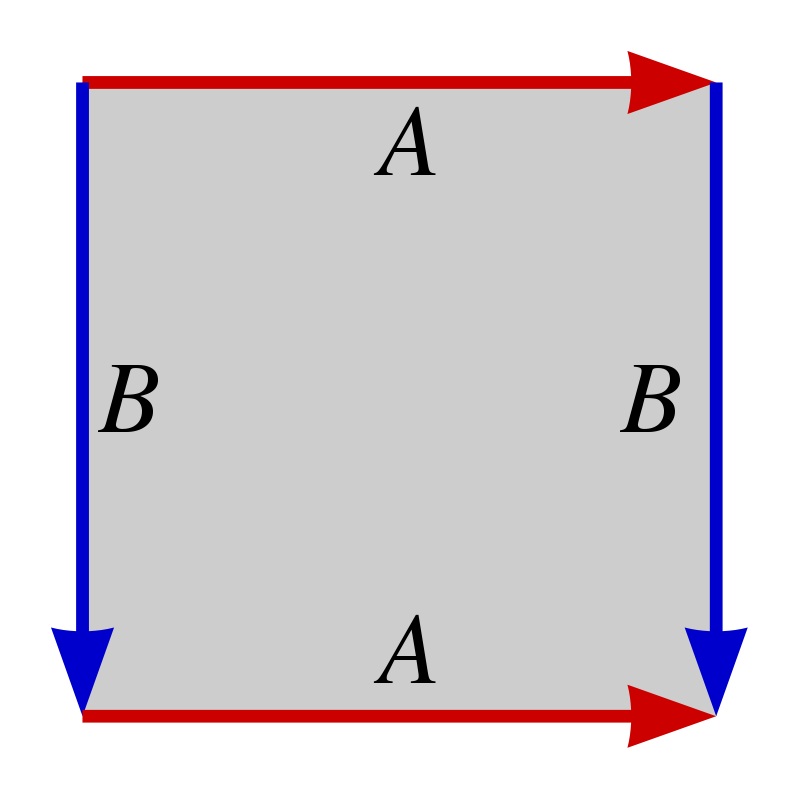
\includegraphics[width=0.2\textwidth]{torus}}
    \qquad
    \subfloat{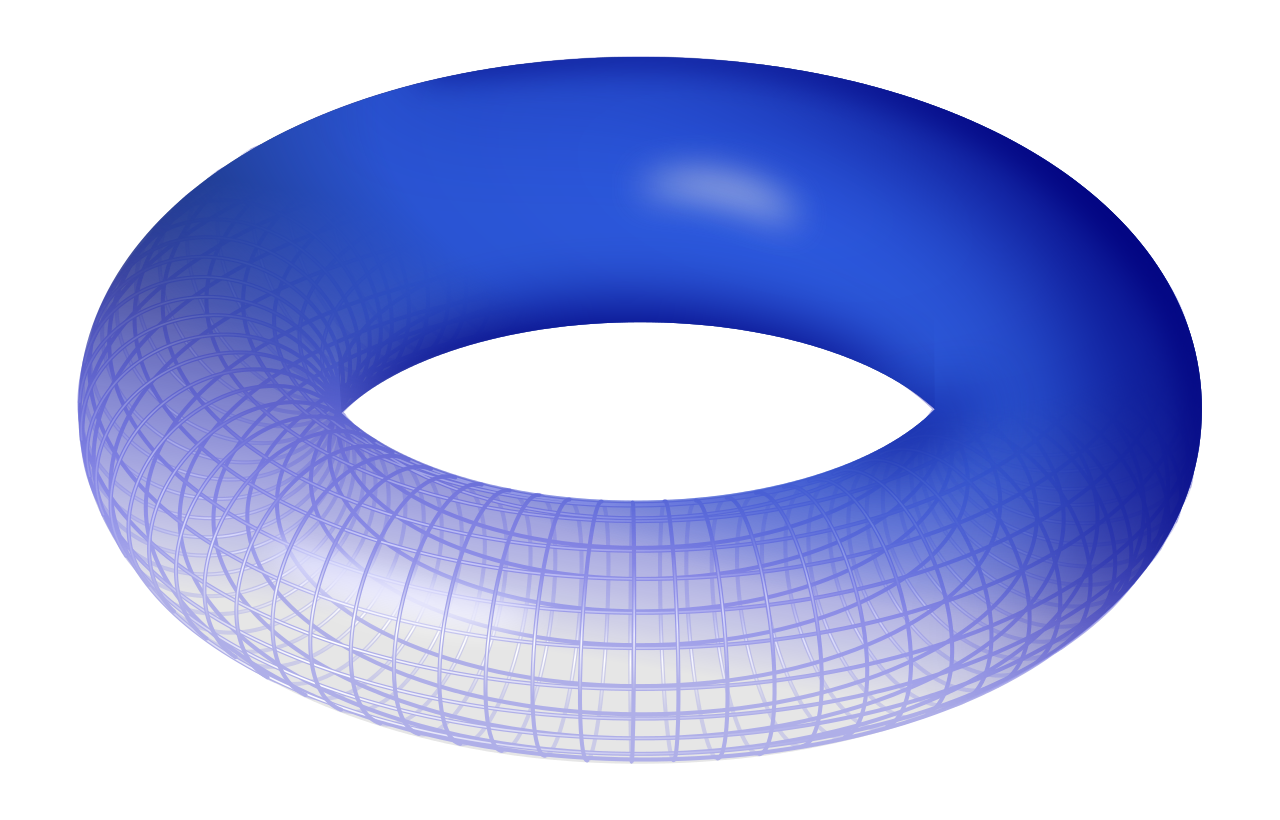
\includegraphics[width=0.2\textwidth]{torus2}}
\end{figure*}

However, it's not obvious whether we can glue the opposing sides like on the next figure.
This is the so-called Klein bottle:

\begin{figure*}[h]
    \centering
    \subfloat{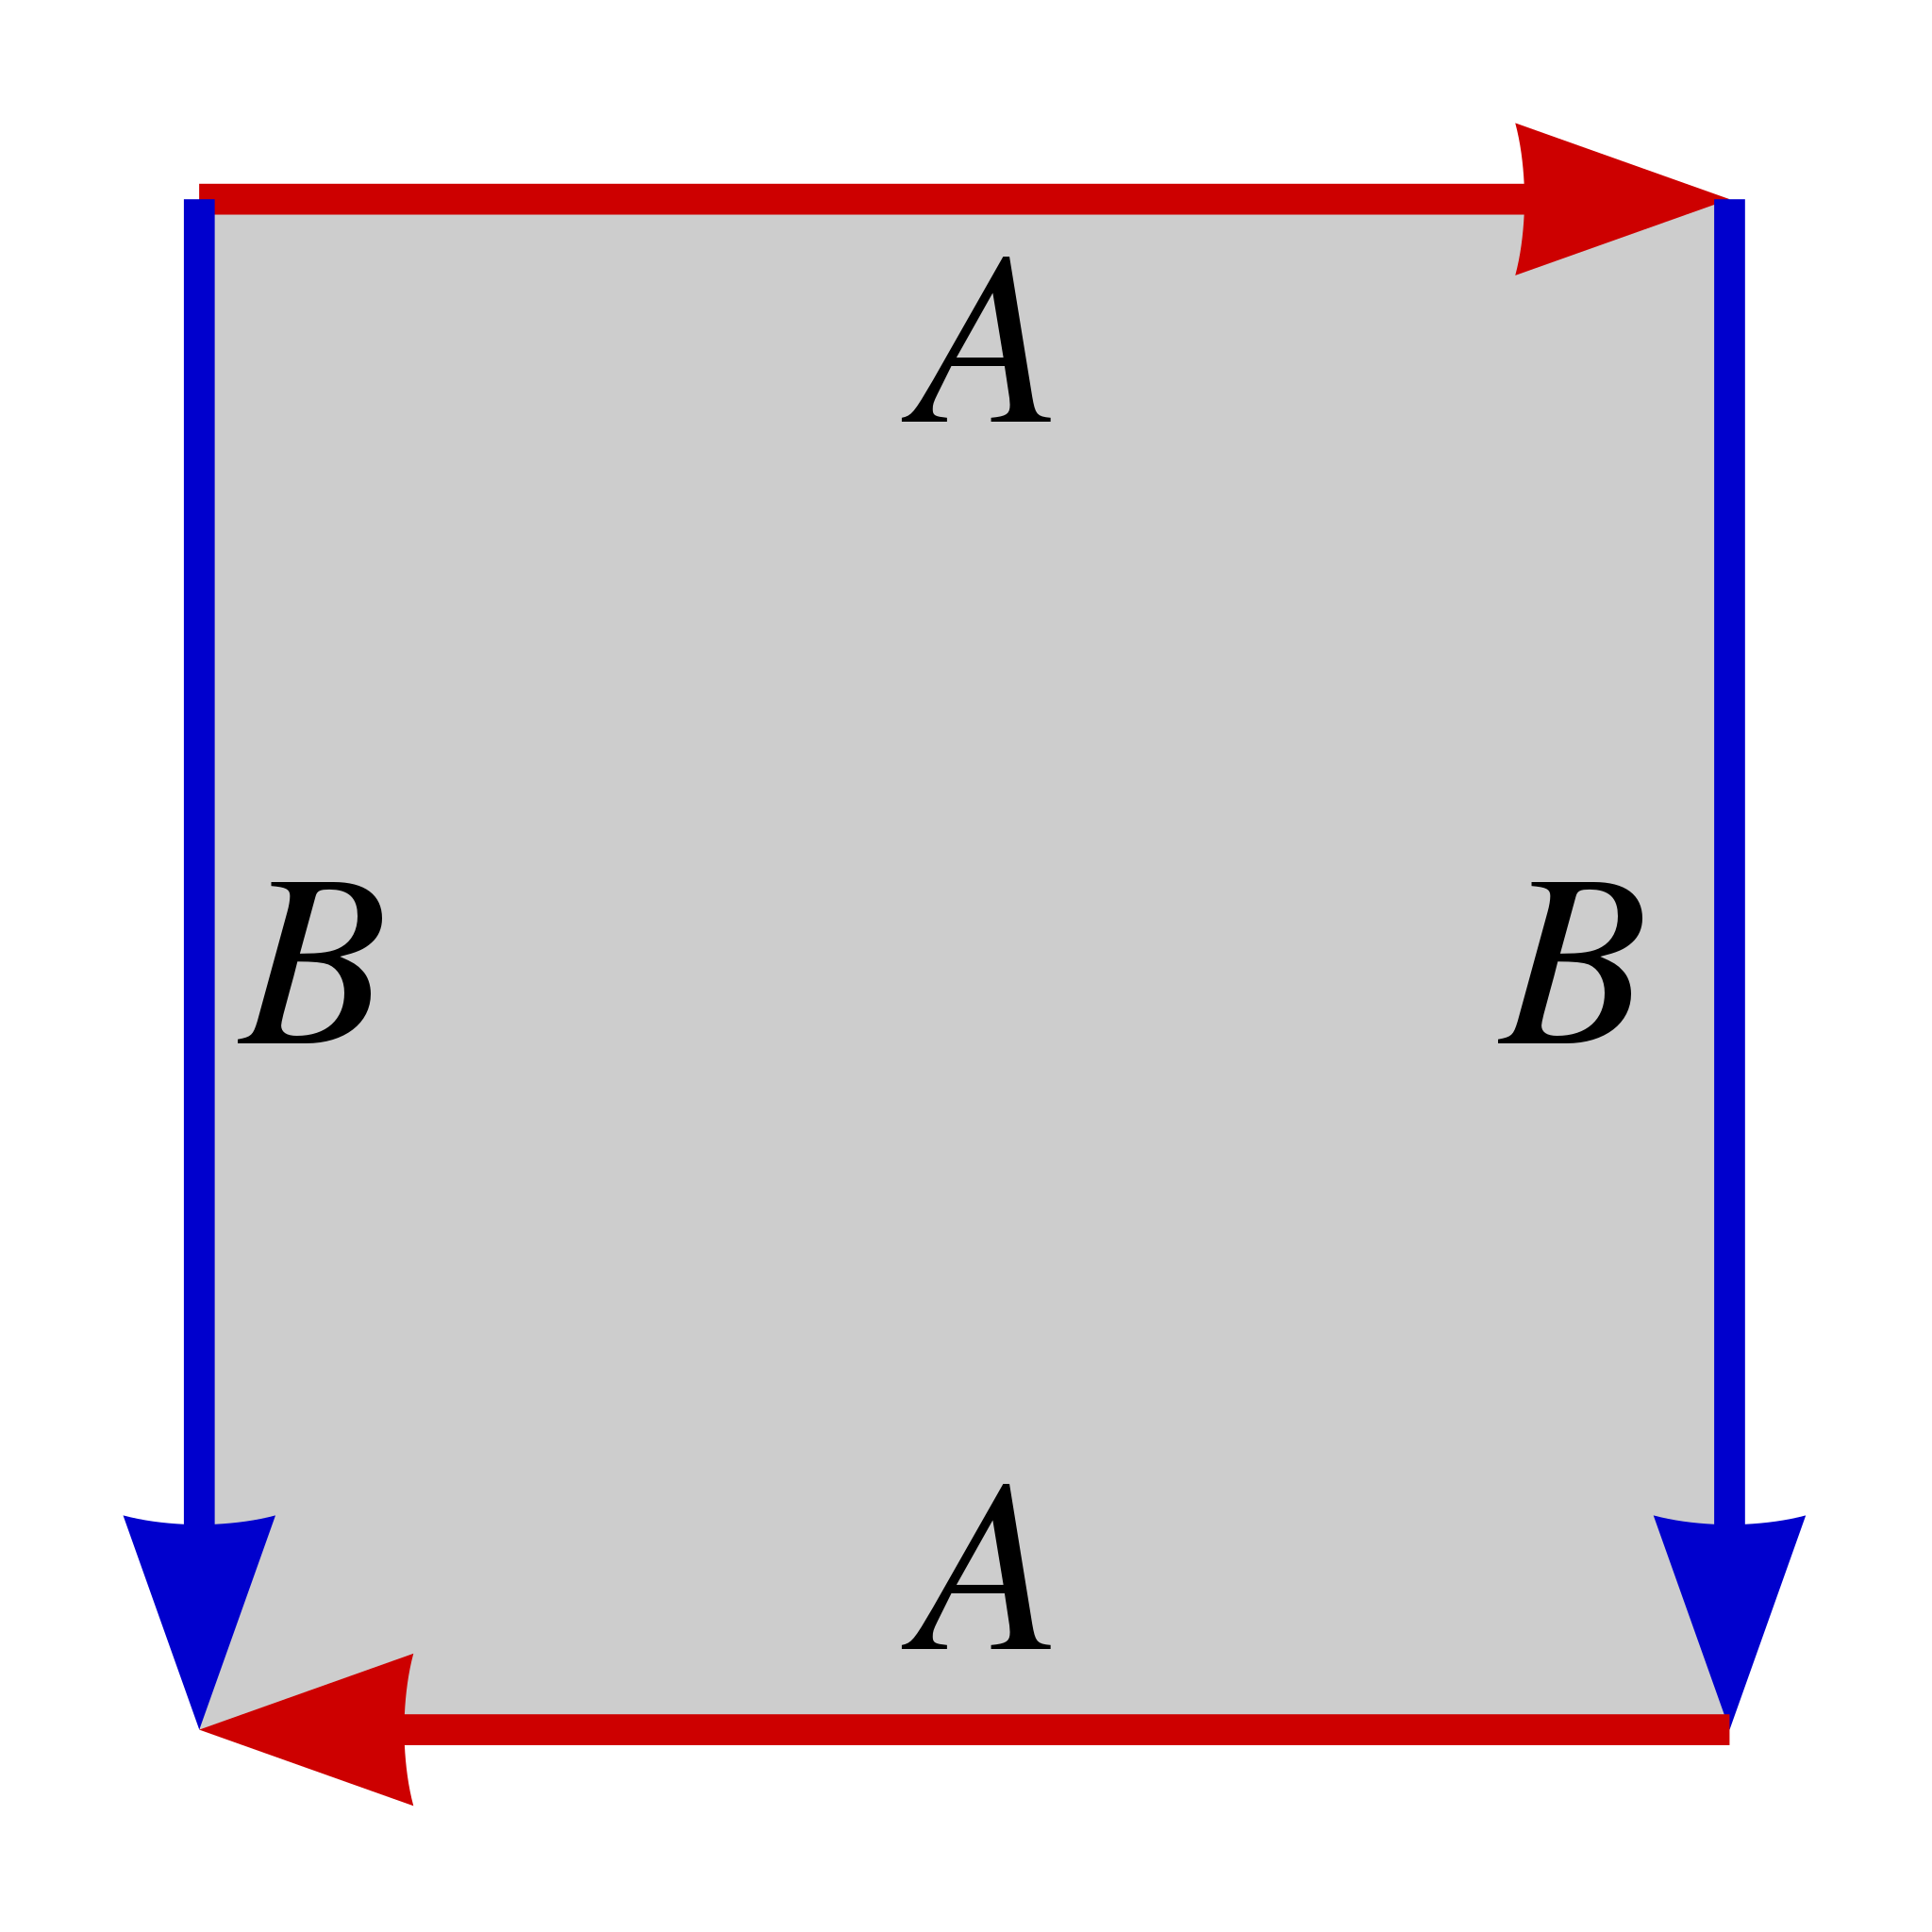
\includegraphics[width=0.2\textwidth]{klein}}
    \qquad
    \subfloat{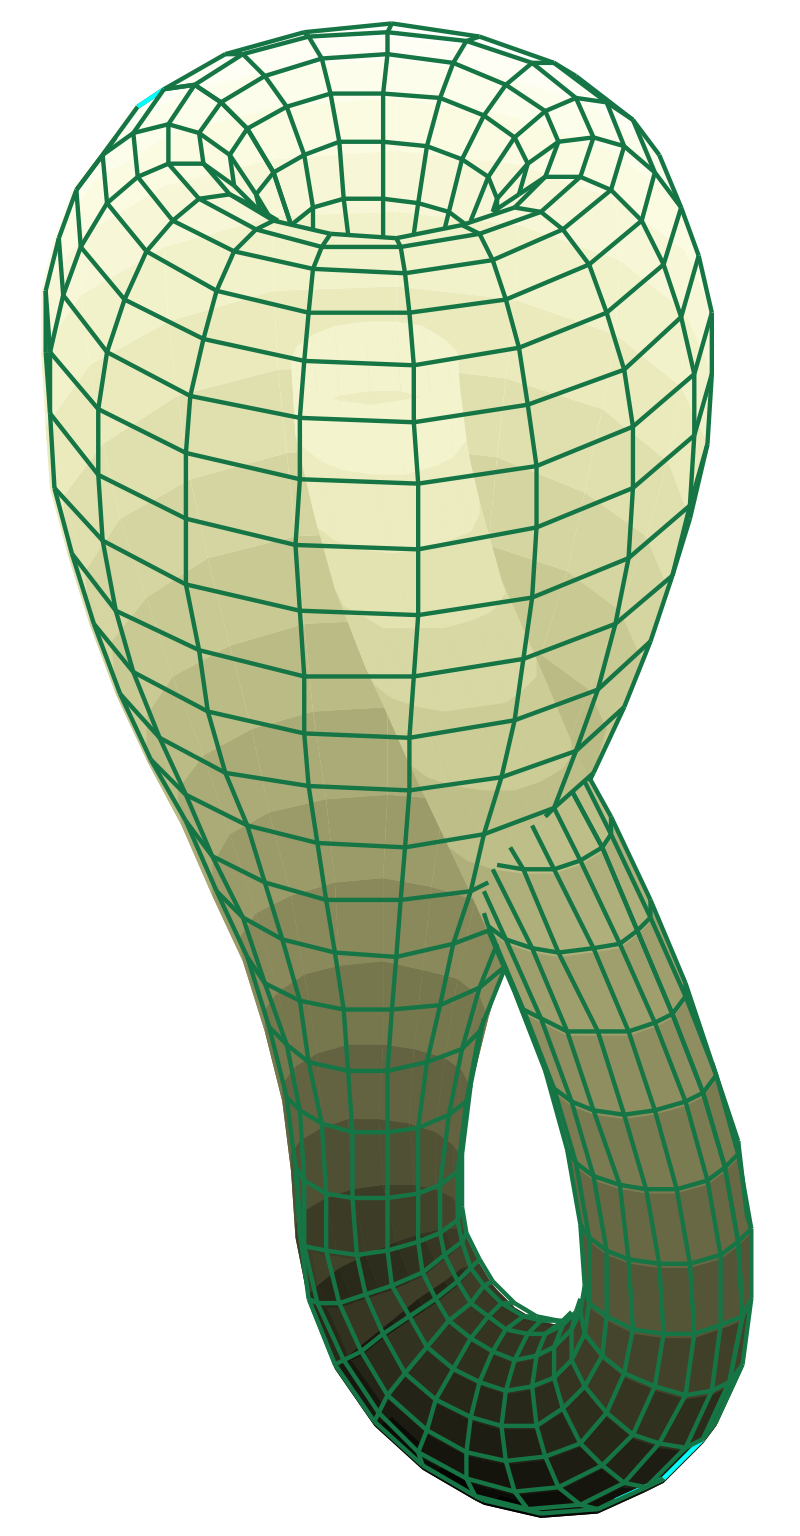
\includegraphics[width=0.13\textwidth]{klein2}}
\end{figure*}

At every point of the surface it looks like $\mathbb{R}^2$!

\subsection{Review of topology}
\begin{definition}[Topological space]
    $X$ --- a set, $\tau = \{U_\alpha \subset X\}_{\alpha \in I}$
    ($I$ --- some index set).
    \begin{enumerate}
        \item {
            $\emptyset, X \in \tau$.
        }
        \item {
            Arbitrary unions of sets from $\tau$ are in $\tau$.
        }
        \item {
            Finite intersections of sets from $\tau$ are in $\tau$.
        }
    \end{enumerate}
    Then $(X, \tau)$ is a \textit{topological space}.
    $U_\alpha$ are called \textit{open sets}. Each $U_\alpha^C$ is a \textit{closed set}.
\end{definition}
\begin{example}
    If $d(\, \cdot\, , \, \cdot \,)$ is a metric on $X$, then 
    $B_r(x) = \{y \in X \mid d(x, y) < r\}$ and $U \subset X$ is open, 
    if $\forall x \in U: \exists r > 0: B_r(x) \subset U$.
\end{example}

A topological space is the smallest structure on a set that allows us to talk about
convergence: a sequence of points in a set converges to a limit, if
for every open set containing this limit the sequence is contained
in that open set starting from some $N$.

\begin{definition}
    $f : X \to Y$ is \textit{continuous} if the preimage of any open set in $Y$
    is open in $X$.
\end{definition}
\begin{definition}
    A bijection $f : X \to Y$ with $f$ and $f^{-1}$ being continuous is called a
    \textit{homeomorphism}.
\end{definition}
\begin{remark}
    Since $f$ is continuous,
    this means that $f^{-1}$ maps every open set in $Y$ to an open set in $X$.
    But since $f^{-1}$ is continuous as well, this means that 
    $f$ maps every open set in $X$ to an open set in $Y$.

    Therefore, $f$ creates a bijection between open sets in $X$ and in $Y$.
\end{remark}
\begin{example}
    \begin{enumerate}
        \item {
            $
                \arctan: (-\infty, +\infty) \to
                \bigl(-\frac{\pi}{2}, \frac{\pi}{2}\bigr)
            $ is a homeomorphism.
        }
        \item {
            \[
                f: [0, 1) \cup [2, 3] \to [0, 2] \qquad
                f(x) = \begin{cases}
                    x & \text{if } x \in [0, 1)\\
                    x - 1 & \text{if } x \in [2, 3]
                \end{cases}
            \]
            Here we have an induced topology on $[0, 1) \cup [2, 3]$. Is this a homeomorphism?
            \begin{enumerate}
                \item {
                    $f$ is a bijection.
                }
                \item {
                    Is $f$ continuous? We need to check that the preimage of an any open 
                    set $U$ in $[0, 2]$ is open in $[0, 1) \cup [2, 3]$.
                    Part of the preimage will be mapped into $[0, 1)$, and part
                    will be mapped into $[2, 3]$.
                    
                    It can be shown that the left endpoint of $f^{-1}(U \cap [0, 1))$
                    and the right endpoint of $f^{-1}(U \cap [1, 2])$ will be excluded.
                    Therefore, the preimage in question can be represented as
                    \[
                        \bigl(f^{-1}(U \cap [0, 1)),\, f^{-1}(U \cap [1, 2])\bigr)
                        \cap \bigl([0, 1) \cup [2, 3]\bigr)
                    \]
                    As this is an intersection of an open set in $\mathbb{R}$ with
                    our set, then it's open in the induced topology.
                }
                \item {
                    $f^{-1}$ is not continuous.
                    Let's take the set $[2, 3]$. It's open in $[0, 1) \cup [2, 3]$
                    by the definition of an induced topology. However,
                    \[
                        (f^{-1})^{-1}([2, 3]) = f([2, 3]) = [1, 2]
                    \]
                    $[1, 2]$ is not open, therefore, $f^{-1}$ is not continuous.
                }
            \end{enumerate}
        }
    \end{enumerate}
\end{example}

\begin{definition}
    A topological space $(X, \tau)$ is called \textit{Hausdorff}
    if for all $x, y \in X,\, x \ne y$ there are open neighborhoods
    $U$ of $x$ and $V$ of $y$, such that $U \cap V = \emptyset$.
\end{definition}
\begin{example}
    Zariski topology on $\mathbb{R}$ or $\mathbb{C}$:
    $U$ is open if and only if $U = \emptyset$ or $X \setminus U$ is finite.

    It is not Hausdorff: there is no way to construct non-overlapping neighborhoods
    of two different points, because every open set is $X$ without a just a finite number of points,
    which will still leave us with a continuum of common points.
\end{example}

\begin{definition}[Basis]
    $X$ --- set, $\mathcal{B}$ --- collection of subsets of $X$, such that:
    \begin{enumerate}
        \item {
            \[ X = \bigcup_{B \in \mathcal{B}} B, \quad \emptyset \in \mathcal{B} \]
        }
        \item {
            For all $B_1,\, B_2 \in \mathcal{B}$ and
            $x \in B_1 \cap B_2$, there exists a $B_3 \in \mathcal{B}$ with 
            $x \in B_3 \subset (B_1 \cap B_2)$.
        }
    \end{enumerate}
    Then the set of all unions of elements of $\mathcal{B}$ is called the topology 
    generated by $B$.

    Such $\mathcal{B}$ is called a \textit{basis} of the topology it generates.
\end{definition}
\begin{proposition}
    The definition is correct, i.e. this is indeed a topology.
\end{proposition}
\begin{proof}
    \begin{enumerate}
        \item {
            $\emptyset,\, X \in \tau$ --- true, because we can
            take the empty union and the union of all $B \in \mathcal{B}$.
        }
        \item {
            Unions of $U_\alpha$'s from $\tau$ are in $\tau$ --- we can 
            just take the union of the corresponding elements from $\mathcal{B}$.
        }
        \item {
            Let's prove that the intersection of two open sets $U_\alpha$ and $U_\beta$
            is open, then use induction to prove that for finite intersections.

            Let's assume $x \in U_\alpha \cap U_\beta$.
            Since $U_\alpha$ is a union of sets from $\mathcal{B}$, we can 
            choose the one that contains $x$ and call it $B_1$. Let's do the same thing with
            $U_\beta$ and $B_2$. So,
            $x \in B_1 \cap B_2$ where $B_1 \subset U_1,\ B_2 \subset U_\beta$.

            By the definition of $\mathcal{B}$, there exists a
            $B_{3,x} \subset U_\alpha \cap U_\beta$, such that $x \in B_{3,x}$.
            $B_{3,x}$ is open, because it's a union of just one set from $\mathcal{B}$.
            Since $x \in U_\alpha \cap U_\beta$ was arbitrary,
            \[
                U_\alpha \cap U_\beta = \bigcup_{x \in U_\alpha \cap U_\beta} B_{3, x}
            \]
            Therefore, $U_\alpha \cap U_\beta$ as a union of open sets. 
        }
    \end{enumerate}
\end{proof}

\begin{definition}
    A topological space is called \textit{second-countable} if it has a countable basis.
\end{definition}

\begin{proposition}
    Second-countability implies
    \hyperref[def:separable]{separability}.
\end{proposition}
\begin{proof}
    Let's assume we have a second-countable set with a countable basis $\mathcal{B}$.
    Choose an arbitrary point in each element of $\mathcal{B}$ to form
    a countable set in $A$. If $A$ is not dense,
    then there exists an open set $U$, such that $U \cap A = \emptyset$.
    But since $\mathcal{B}$ is a basis, $U$ is some union of elements of 
    $\mathcal{B}$. Let's take one of those elements, $B_U$.
    We've chosen a point $x$ in $B_U$:
    \[
        \begin{cases}
            x \in B_U \subset U\\
            x \in A
        \end{cases} \implies
        x \in U \cap A \implies U \cap A \ne \emptyset \text{?!}
    \]
\end{proof}
\begin{remark}
    The inverse is not true: there are separable sets that are not second-countable.
\end{remark}

\subsection{Manifolds}
\begin{definition}
    $M$ is a \textit{topological manifold of dimension $n$}
    if it is a Hausdorff and second-countable topological space, such that
    every point in $M$ has a neighborhood homeomorphic to an open set in
    $\mathbb{R}^n$.

    (For all $p \in M$ there exists an open $U \subset M$,
    such that $p \in U$ and there exist an open $V \in \mathbb{R}^n$ and
    a homeomorphism $\varphi : U \to V$.)
\end{definition}
\begin{remark}
    This definition would work for a Klein bottle. Locally around every point
    it looks like a plane.
\end{remark}
\begin{remark}
    It turns out that the number $n$ is a topological invariant, i.e.
    two topological manifolds cannot be homeomorphic if their dimensions differ.
    
    Exercise: reduce this to the following statement:
\end{remark}
\begin{theorem}[Brower's invariance of domain]
    Let $U \subset \mathbb{R}^n$ be open, and let $f : U \to \mathbb{R}^n$
    be continuous and injective. Then $f(U)$ is open in $\mathbb{R}^n$.
\end{theorem}
We're not gonna prove this theorem.
Let's look at a simpler case: a continuous injective function in $\mathbb{R}$.
$f : \mathbb{R} \to \mathbb{R}$. If $f \in C^1(\mathbb{R})$, then
\[ f(x) = f(x_0) + f'(x_0)(x - x_0) + o(\abs{x - x_0}) \]
If $f'(x_0)$ is not zero,
it follows that $f(x_0)$ cannot be a boundary point, since 
$ f(x) - f(x_0)$ will have two different signs around $x_0$.
But again, $f'(x_0)$ can have zeros, so this is not a full proof.

\begin{samepage}
\begin{definition}
    A pair $(U, \varphi)$ with $U \subset M$ --- an open set and
    $\varphi: U \to \mathbb{R}^n$ --- a homeomorphism from
    $U$ to $\varphi(U) = V$ is called a \textit{chart}.
    \begin{itemize}
        \item {
            $\varphi$ is a local coordinate map.
        }
        \item {
            $\varphi(p) = \bigl(x^1(p), x^2(p), \dots, x^n(p)\bigr)$ --- local
            coordinates. They don't work on the whole $M$ --- just on $U$.
        }
        \item {
            $\varphi^{-1} : V \to U$ is called a \textit{coordinate system}.
        }
    \end{itemize}
\end{definition}
\end{samepage}
Examples of topological manifolds:
\begin{enumerate}
    \item {
        An open set in $\mathbb{R}^n$. We only need one chart --- $\mathbb{R}^n$ itself.
    }
    \item {
        The $n$-sphere 
        \[
             S^n \coloneqq \{ (x^1, \dots, x^{n+1}) \in \mathbb{R}^{n+1}
             \mid {\textstyle \sum} (x^j)^2 = 1 \} 
        \]
        We would need two charts. Let's have one chart as
        the sphere except the north pole with homeomorphism as a stereographic projection,
        and the other as the sphere except the south pole.
        The two charts overlap, but they still satisfy the definition.

        \begin{figure*}[h]
            \centering
            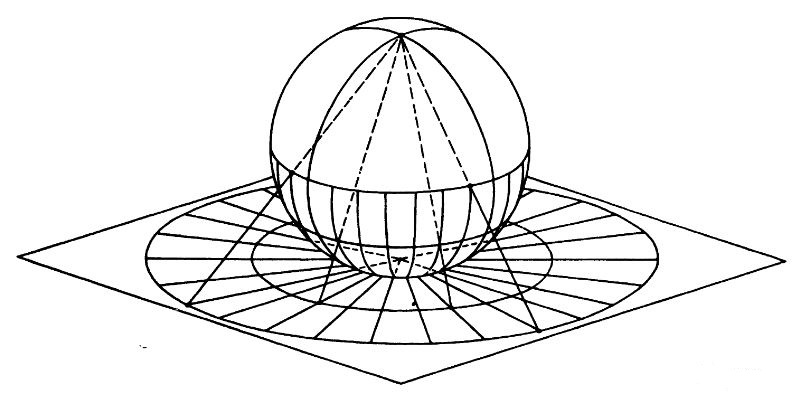
\includegraphics[width=0.4\textwidth]{stereographic}
        \end{figure*}
    }
    \item {
        $\mathbb{P}^n$ --- projective space.
        $\mathbb{P}^n = \bigl(\mathbb{R}^n \setminus \{0\} \bigr) / \sim$.
        (We're gonna define $\sim$ later).

        $\mathbb{P}^1$ --- the set of all lines in $\mathbb{R}^2$ passing through
        the origin:
        \begin{center}   
            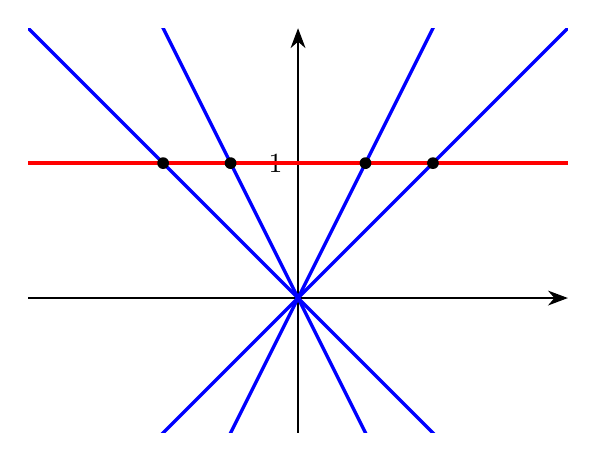
\begin{tikzpicture}
                \begin{axis}[
                    axis x line=center,
                    axis y line=center,
                    axis line style={-{Stealth[scale=1.5]}},
                    ytick={1},
                    xtick=\empty,
                    xmin=-2, xmax=2, ymin=-1, ymax=2,
                    unit vector ratio=1 1 1,
                    samples=100,
                ]
                    \tikzset{graph/.style={very thick, smooth, domain=-2:2}}
                    \tikzset{graph_point/.style={fill,circle,inner sep=1.5pt}}
                    \addplot[red, graph] {1};
                    \addplot[blue, graph] {x};
                    \addplot[blue, graph] {-x};
                    \addplot[blue, graph] {2 * x};
                    \addplot[blue, graph] {-2 * x};
                    \node[graph_point] at (1, 1){};
                    \node[graph_point] at (0.5, 1){};
                    \node[graph_point] at (-0.5, 1){};
                    \node[graph_point] at (-1, 1){};
                \end{axis}
            \end{tikzpicture}
        \end{center}
        Every non-horizontal line passing through the origin can be mapped onto 
        a point on the red line. A horizontal line corresponds to the 
        point at infinity. So, essentially, $\mathbb{P}^1$ 
        is equivalent the extended real line. 

        Here's how we're gonna define our equivalence relation:
        $(x_1, y_1) \sim (x_2, y_2)$ if and only if $x_1 = kx_2$ and $y_1 = ky_2$,
        i.e. if they're on the same line:
        \begin{center}   
            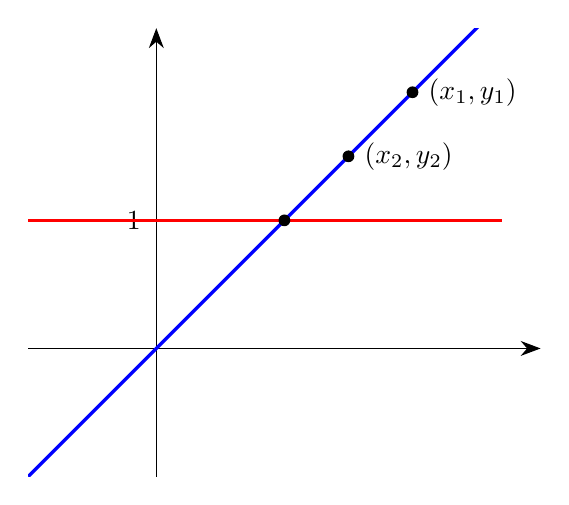
\begin{tikzpicture}
                \begin{axis}[
                    axis x line=center,
                    axis y line=center,
                    axis line style={-{Stealth[scale=1.5]}},
                    ytick={1},
                    xtick=\empty,
                    xmin=-1, xmax=3, ymin=-1, ymax=2.5,
                    unit vector ratio=1 1 1,
                    samples=100,
                ]
                    \tikzset{graph/.style={very thick, smooth, domain=-1:2.7}}
                    \tikzset{graph_point/.style={fill,circle,inner sep=1.5pt}}
                    \addplot[red, graph] {1};
                    \addplot[blue, graph] {x};
                    \node[graph_point] at (1, 1){};
                    \node[graph_point,label=0:{$(x_2, y_2)$}] at (1.5, 1.5){};
                    \node[graph_point,label=0:{$(x_1, y_1)$}] at (2, 2){};
                \end{axis}
            \end{tikzpicture}
        \end{center}
        This equivalence relation can be exteneded to $\mathbb{R}^{n+1}$.

        Now, here's how we're gonna define the charts.
        $p \in \mathbb{P}^n \implies$ take a representative
        $(x_1, \dots, x_{n+1})$. Choose $x_i \ne 0$.
        Without the loss of generality, $i = n + 1$, therefore, in some
        neighborhood $U$ around $p$ we have $x_{n + 1} \ne 0$.
        For each point in $U$:
        \[
            \Bigl(\frac{y_1}{y_{n+1}}, \frac{y_2}{y_{n+1}}, \dots, \frac{y_n}{y_{n - 1}}, 1\Bigr)
            \sim (y_1, \dots, y_{n + 1})
        \]
        So, around every point of the projective space we can find a chart:
        take any representative of that point, find a non-zero coordinate.
        This coordinate will remain non-zero in some neighborhood, therefore,
        we can divide by it, and this coordinate by which we divide 
        will turn to $1$. The remaining $n$ coordinates will define the coordinates of a point
        in $\mathbb{R}^n$, which will provide a local homeomorphism around
        the point in the projective space to a subset $\mathbb{R}^n$, 
        which defines a chart.
    }
\end{enumerate}
\subsection{Smooth manifolds}

Let's say we have two intersecting charts: $U_1$ and $U_2$
with maps $\varphi_1$ and $\varphi_2$.
Each of those charts are mapped onto $\mathbb{R}^n$ by their respective local
coordinate maps.
If we consider $U_1 \cap U_2$, we can consider how it's mapped onto $\mathbb{R}^n$
by $\varphi_1$ and $\varphi_2$:

\begin{figure*}[h]
    \centering
    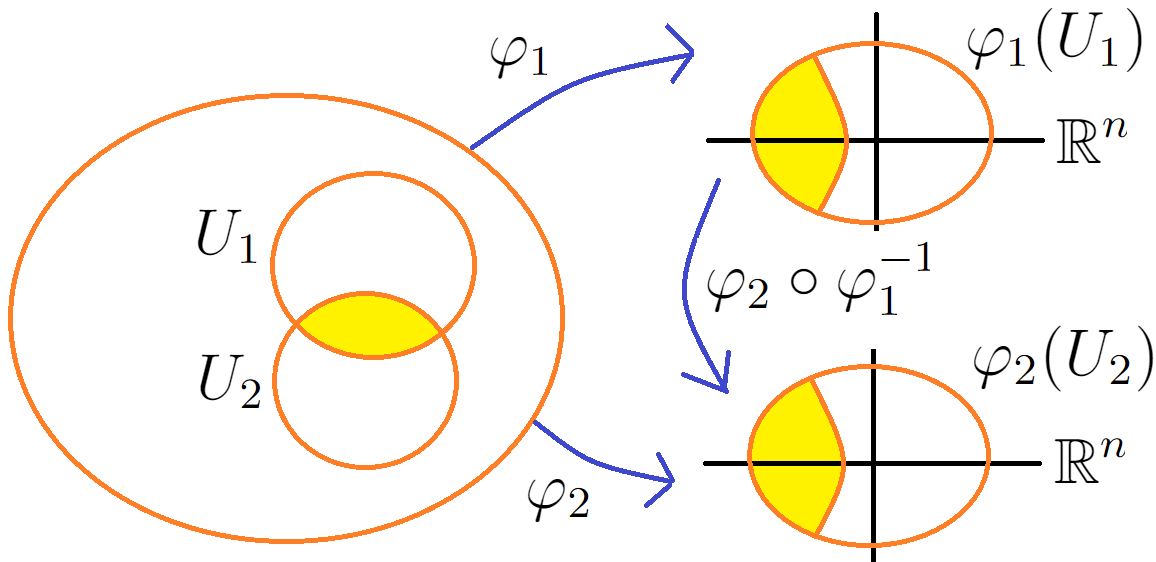
\includegraphics[width=0.7\textwidth]{charts}
\end{figure*}

Since $\varphi_1$ and $\varphi_2$ are both homeomorphisms,
$\varphi_2 \circ \varphi_1^{-1}$ is also a homeomorphism. It will
convert the coordinates of $U_1 \cap U_2$ in the first and in the second chart.

\begin{samepage}
\begin{definition}
    Let $M$ be a topological manifold. 
    Let $\mathcal{A} = \{(U_\alpha, \varphi_\alpha)\}_{\alpha \in I}$, such that:
    \begin{enumerate}
        \item {
            $U_\alpha$ are open and cover $M$.
        }
        \item {
            For all $\alpha, \beta$ with $U_\alpha \cap U_\beta \ne \emptyset$,
            the \textit{transition map}
            \[ 
                \varphi_\beta \circ \varphi_\alpha^{-1} :
                \varphi_\alpha(U_\alpha \cap U_\beta) \to \varphi_\beta(U_\alpha \cap U_\beta)
            \]
            is $C^r$-smooth (i.e., it has $r$ continuous derivatives).
        }
    \end{enumerate}
    Then $\mathcal{A}$ is called a \textit{$C^r$-atlas} of M,
    and the pair $(M, \mathcal{A})$ is called a \textit{$C^r$-manifold}.
\end{definition}
\end{samepage}
\begin{remark}
    This definition is different from the definition of a topological manifold,
    in that now we care about how we glue the charts together --- we want
    it to be smooth.
    If we were to talk about smooth functions on a manifold, then 
    we would run the computations separately on each chart. But in order for 
    those computations to agree with each other, we would need the transition
    functions to be smooth as well.
\end{remark}
\begin{remark}
    By \textit{smooth}  we will mean $C^\infty$-smooth.
\end{remark}

\begin{definition}
    A \textit{$C^r$-differentiable structure} on $M$ is a maximal $C^r$-atlas on
    $\mathcal{A}$ (i.e., not contained in any other $C^r$-atlas).
\end{definition}
\begin{definition}
    Two $C^r$-atlases $\mathcal{A}_1$ and $\mathcal{A}_2$ are \textit{$C^r$-equivalent}, 
    if $\mathcal{A}_1 \cup \mathcal{A}_2$ is a $C^r$-atlas.
\end{definition}
\begin{proposition}
    $C^r$-equivalence is an equivalence relation.
\end{proposition}
\begin{lemma}
    The union of all $C^r$-equivalent atlases in a single equivalence class is
    a maximal atlas. Hence, a maximal atlas exists.
\end{lemma}
\begin{remark}
    We leave the proofs as an exercise.
\end{remark}

There are atlases that don't admit a smooth structure!
For $n = 1, 2, 3, 5, 6$, the $n$-dimensional sphere has only one
smooth structure (i.e. $C^\infty$-differentiable structure).
If $n = 7$ --- there are 28.

Examples of smooth manifolds:
\begin{enumerate}
    \item {
        $\mathbb{R}^n$ --- it has a single chart.
    }
    \item {
        Any open subset of a smooth manifold is a smooth manifold
        (we can intersect the charts with our subset).
    }
    \item {
        A graph of a smooth function $f : \mathbb{R}^n \to \mathbb{R}$.
    }
    \item {
        A sphere $S^n$. We can obtain at least one smooth structure
        using two stereographic projections (as before). The exercise is to check that
        the resulting conversion between those two charts is smooth.
    }
    \item {
        A real projective space $\mathbb{P}^n$. 
        We have defined $\mathbb{P}^n$ before as
        $(x_0, x_1, \dots, x_n) / \sim$ with $n + 1$ different charts,
        depending on which coordinate of a given vector is non-zero.
    }
\end{enumerate}

\begin{remark}
    The smooth structure does not define distances on the manifold.
\end{remark}

\pagebreak
\subsection{Smooth maps between manifolds}
TODO: insert picture.

\begin{definition}
    Let $M$, $N$ be smooth manifolds.
    A map $f : M \to N$ is \textit{smooth} at $p \in M$,
    if there exist charts $(U, \varphi)$ with $p \in U$ and
    $(V, \psi)$ with $f(p) \in V$, such that $f(U) \subset V$ and
    $\psi \circ f \circ \phi^{-1} : \varphi(U) \to \psi(V)$
    is smooth (i.e. infinitely many times differentiable) at $\varphi(p)$.
\end{definition}
\begin{remark}
    The key idea is that if we forget about the maps to $\mathbb{R}^m$/$\mathbb{R}^n$
    and focus solely on $M$ and $N$ themselves, then we simply won't have enough
    structure to define the smoothness of a function.
\end{remark}
\begin{definition}
    $f : M \to N$ is smooth, if it is smooth at every point of $M$.
\end{definition}
\begin{remark}
    If $U \subset \mathbb{R}^m$, then $f : U \to \mathbb{R}^n$
    is smooth if all partial derivatives exist.
\end{remark}
\begin{lemma}
    \label{lem:independentOfChartChoice}
    Smoothness of $f : M \to N$ is independent of the choice of 
    charts in the definition, as long as $f(U) \subset V$.
\end{lemma}
\begin{proof}
    We'll only give the proof idea.
    If we choose other charts, we'll get different $\psi$ and $\phi$ in 
    $\psi \circ f \circ \phi^{-1}$. In order to go back to the original
    $\psi$ and $\phi$, we'll have to compose with the transition maps,
    which are smooth because $M$ and $N$ are smooth manifolds,
    therefore the smoothness is preserved.
\end{proof}
\begin{proposition}
    If $M$, $N$ are smooth manifolds and
    $f : M \to N$ is smooth, then $f$ is continuous (i.e. the preimage of 
    an open set is open),
\end{proposition}
\begin{proof}
    Let's prove it for any point $p \in M$.
    Let's suppose again that $p$ is part of the chart $(U, \varphi)$,
    and $f(p)$ is part of the chart $(V, \psi)$.
    Then we can represent $f|_U$ as
    \[
        f|_U = \varphi^{-1} \circ (\psi \circ f \circ \varphi^{-1}) \circ \varphi
    \]
    $\varphi^{-1}$ is continuous, as it is a homeomorphism. So is $\varphi$.
    $\psi \circ f \circ \varphi^{-1}$ is also continuous, because it is
    smooth in the sense of calculus (i.e. it's a map from $\mathbb{R}^m$ to $\mathbb{R}^n$).
    Therefore, $f|_U$ is continuous as a composition of three continuous functions.

    Therefore, $f$ is continuous at any point $p \in M$, which means that
    $f$ is continuous.
\end{proof}
\begin{proposition}
    \label{prop:propTwoIdk}
    \begin{enumerate}
        \item {
            If $f : M \to N$ and $g : N \to P$ are smooth, then 
            $g \circ f : M \to P$ is smooth.
        }
        \item {
            If $f, g : M \to \mathbb{R}^n$, $\lambda : M \to \mathbb{R}$
            are smooth, then $f + g$, $\lambda g$ and
            $\langle f, g \rangle = \sum f_i(g) \cdot g_i(x)$ are
            smooth functions.
        }
    \end{enumerate}
\end{proposition}
\begin{proof}
    This can be done by the direct application of the definition.
\end{proof}
\begin{definition}[Diffeomorphism]
    Let $M$, $N$  be smooth manifolds. A bijection $f : M \to N$,
    such that $f$ and $f^{-1}$ are smooth is called a 
    \textit{diffeomorphism}.
\end{definition}
\begin{example}
    It can be proved that all compact connected manifolds of dimension 1
    in $\mathbb{R}^2$ are diffeomorphic to a circle.
\end{example}

\subsection{Tangent spaces}
\subsubsection*{Model case}
$M \subset \mathbb{R}^{n+1}$ is a surface given by the graph
of a smooth map $F : \mathbb{R}^n \to \mathbb{R}$.
\[ 
    F(\vec{x} + \vec{v}) = F(\vec{x}) + \nabla F(\vec{x}) \cdot \vec{v} + 
    \textcolor{red}{\vec{o}(\norm{\vec{v}})}
\]
The first two terms are the linear part. They define the tangent space at the point $(\vec{x}, F(\vec{x}))$.
\[
    \nabla F =\Bigl( \frac{\partial F}{\partial x_1}, \dots, 
    \frac{\partial F}{\partial x_n} \Bigr)
    \qquad
    \nabla F(\vec{x}) \vec{v} = \frac{d}{dt} F(\vec{x} + t\vec{v})\Big|_{t=0} =
    D_{\vec{v}} F(\vec{x})
\]
\subsubsection*{General case}
Observe that for $f, g : \mathbb{R}^n \to \mathbb{R}$:
\[ 
    D_{\vec{v}} (fg)(x) = f(x) D_{\vec{v}}(g)(x) + 
    g(x) D_{\vec{v}}(f)(x) 
\]
\begin{definition}
    Let $M$ be a smooth manifold. 
    Let $C^\infty(M)$ denote the space of all $C^\infty$-smooth maps 
    $f: M \to \mathbb{R}$.
\end{definition}
\begin{remark}
    $C^\infty(M)$ is a vector space (by Proposition~\ref{prop:propTwoIdk}),
    and it is not dependent on the choice of charts
    (by Lemma~\ref{lem:independentOfChartChoice}).
\end{remark}
\begin{definition}[Tangent space]
    If $p \in M$, a linear map $D : C^\infty(M) \to \mathbb{R}$ is called a
    \textit{derivation at $p$} if 
    \[ D(fg) = f(p) D(g) + g(p) D(F) \]
    for any $f, g \in C^\infty(M)$.
    Then $T_p M \coloneqq \{D : D \text{ is a derivation at } p \}$
    is called the \textit{tangent space} to $M$ at $p$.
\end{definition}
\begin{lemma}
    Every derivation on $C^\infty(M \subset \mathbb{R}^n)$ at $p$ is some directional
    derivative evaluated at $p$.
\end{lemma}
\end{document}
